\documentclass{beamer}

\usepackage{xltxtra} 
\usepackage{xgreek} 
\usepackage{graphicx}
\usepackage{float}
\usepackage{algpseudocode,algorithm,algorithmicx}
\usepackage{fontspec}
\usepackage{array}

\usetheme{Madrid}
\usecolortheme{whale}

\usefonttheme{professionalfonts} % using non standard fonts for beamer
\usefonttheme{serif} % default family is serif
\setmainfont{GFS Didot} 

\makeatletter
\defbeamertemplate*{footline}{Dan P theme}
{
  \leavevmode%
  \hbox{%
  \begin{beamercolorbox}[wd=.2\paperwidth,ht=2.25ex,dp=1ex,center]{author in head/foot}%
    \usebeamerfont{author in head/foot}\insertshortauthor\expandafter\beamer@ifempty\expandafter{\beamer@shortinstitute}{}{~~(\insertshortinstitute)}
  \end{beamercolorbox}%
  \begin{beamercolorbox}[wd=.6\paperwidth,ht=2.25ex,dp=1ex,center]{title in head/foot}%
    \usebeamerfont{title in head/foot}\insertshorttitle
  \end{beamercolorbox}%
  \begin{beamercolorbox}[wd=.2\paperwidth,ht=2.25ex,dp=1ex,right]{date in head/foot}%
    \usebeamerfont{date in head/foot}\insertshortdate{}\hspace*{2em}
\insertframenumber{} / \inserttotalframenumber\hspace*{2ex} 
  \end{beamercolorbox}}%
  \vskip0pt%
}
\makeatother

\def\todayshort{\leavevmode\hbox{\twodigits\day-\twodigits\month-\the\year}}
\def\twodigits#1{\ifnum#1<10 0\fi\the#1}

\newcommand*\Let[6]{\State #1 $\gets$ #2}  
\algrenewcommand\algorithmicrequire{\textbf{Είσοδος}}  
\algrenewcommand\algorithmicensure{\textbf{Έξοδος}}

\makeatletter  % Add this!!!!
 \renewcommand{\ALG@name}{Αλγόριθμος} %doesnt work
\makeatother   % Add this also
\renewcommand{\listalgorithmname}{Λίστα Αλγορίθμων}

\title[Προηγμένες Τεχνικές Επεξεργασίας Σήματος]{Προηγμένες Τεχνικές Επεξεργασίας Σήματος}
 
\subtitle{Δεύτερη Εργασία 2017-2018}
 
\author[Γραικός Α. Θώμος Μ.]{Γραικός Αλέξανδρος 8128 \\ Θώμος Μάριος 8384}
 
\date[\todayshort]{\today}
 
\begin{document}
 
\frame{\titlepage}

\begin{frame}
\frametitle{Περιεχόμενα}
\tableofcontents
\end{frame}
 
% --- Περιγραφή σημάτων ---
\begin{frame}
\frametitle{Σήματα που επιλέχθηκαν}
\section{Σήματα που επιλέχθηκαν}

\centering
\resizebox{.95\textwidth}{!}{
\begin{tabular}{ >{\centering\arraybackslash}m{1cm} | >{\centering\arraybackslash}m{15cm}} 
\hline
\textbf{112} & Φυσιολογικό σήμα ECG. Θα αναλύσουμε το σήμα και των δύο ακροδεκτών. \\
\hline
\textbf{123} & Φυσιολογικό σήμα με χαμηλό καρδιακό ρυθμό. \\
\hline
\textbf{118} & Σήμα ECG που παρουσιάζει RBBB. \\
\hline
\textbf{217} & Σήμα που οδηγείται από βηματοδότη. \\
\hline
\textbf{221} & Σήμα ασθενούς με κολπική μαρμαρυγή. \\
\hline
\end{tabular}}

\centering
\begin{columns}
\column{0.5\textwidth}
\begin{figure}
\includegraphics[width=\textwidth, trim={0 6cm 0 6cm}, clip]{fig/pres_sig1.pdf}
\end{figure}

\column{0.5\textwidth}
\begin{figure}
\includegraphics[width=\textwidth, trim={0 6cm 0 6cm}, clip]{fig/pres_sig2.pdf}
\end{figure}
\end{columns}

\end{frame}



% --- Ανάλυση 112 (lead 1) ---
\section{Ανάλυση Σημάτων}
\subsection{Σήμα 112 (Ακροδέκτης 1)}
\begin{frame}
\frametitle{Ανάλυση των σημάτων - 112 (Ακροδέκτης 1)}

\begin{columns}
\column{0.5\textwidth}
\begin{figure}
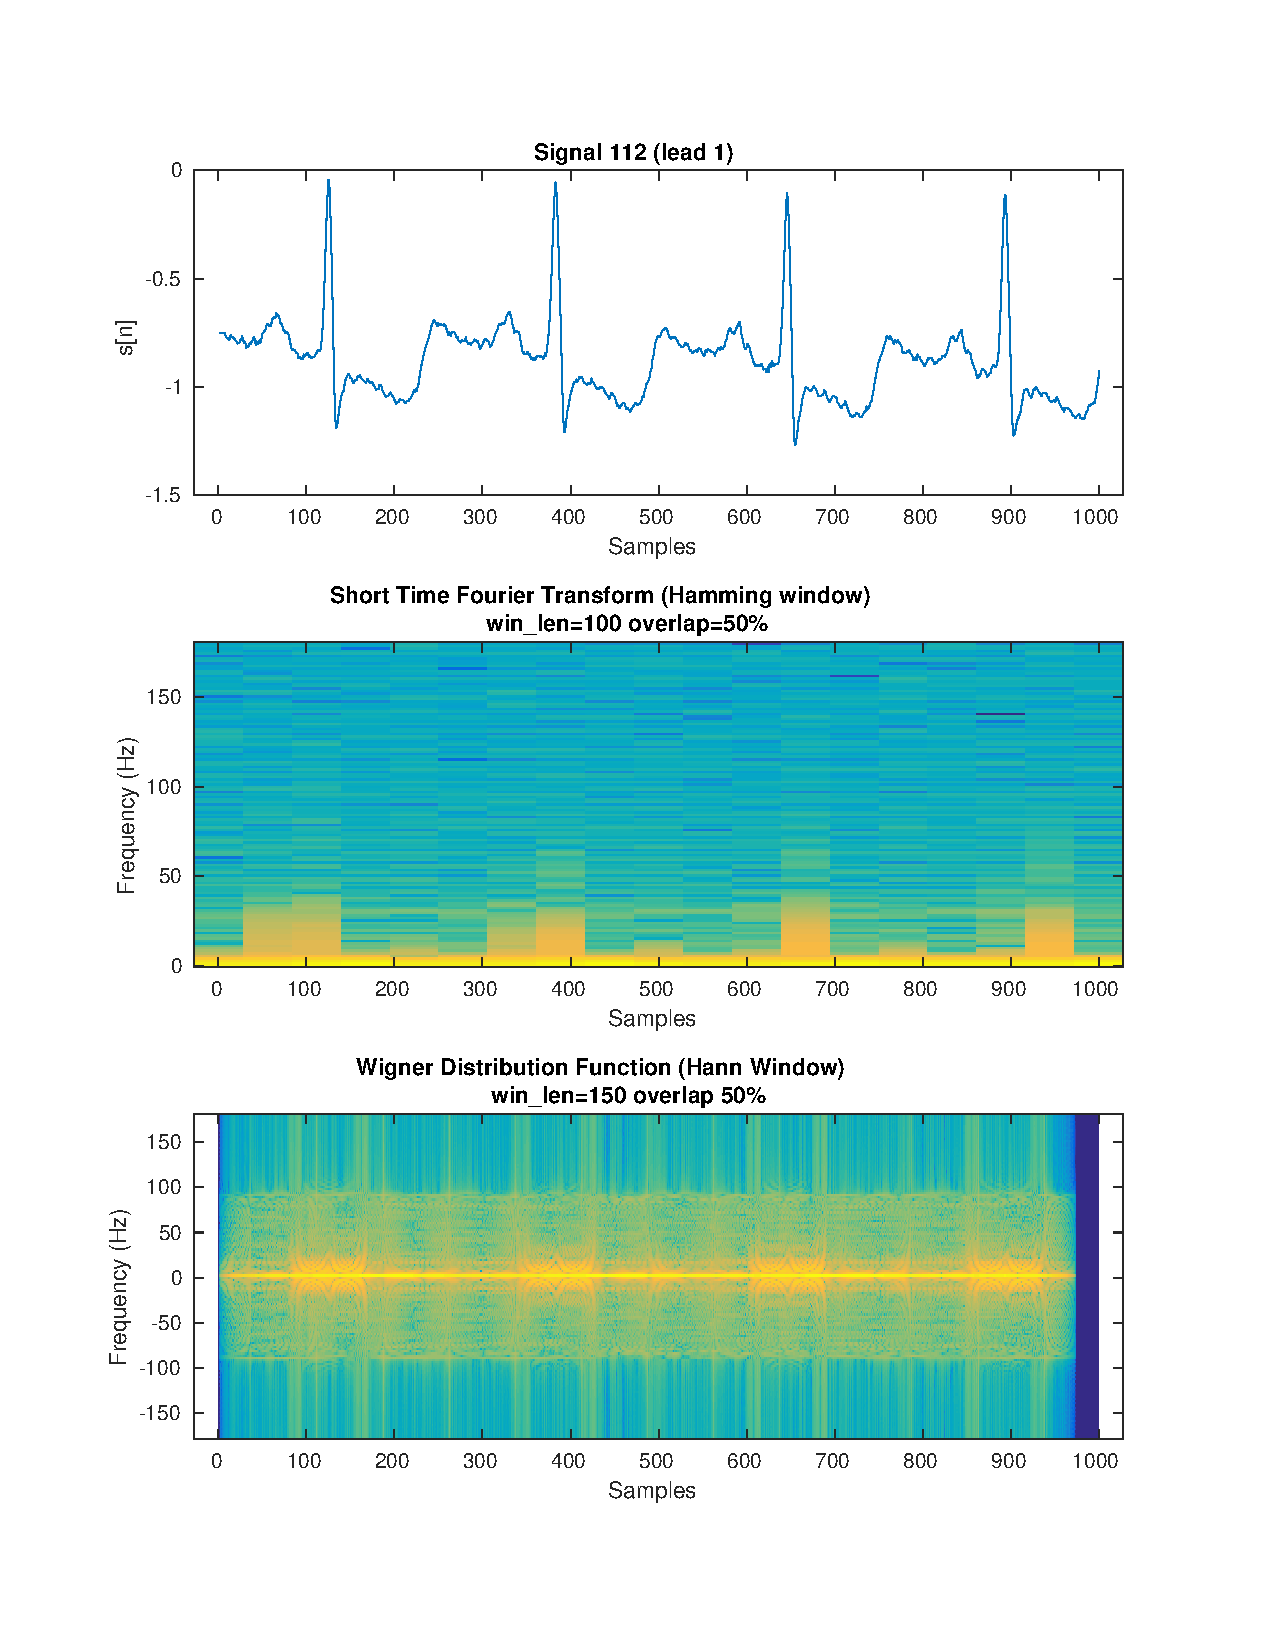
\includegraphics[width=\textwidth]{fig/112l1_stft_wdf.pdf}
\end{figure}

\column{0.5\textwidth}
\begin{figure}
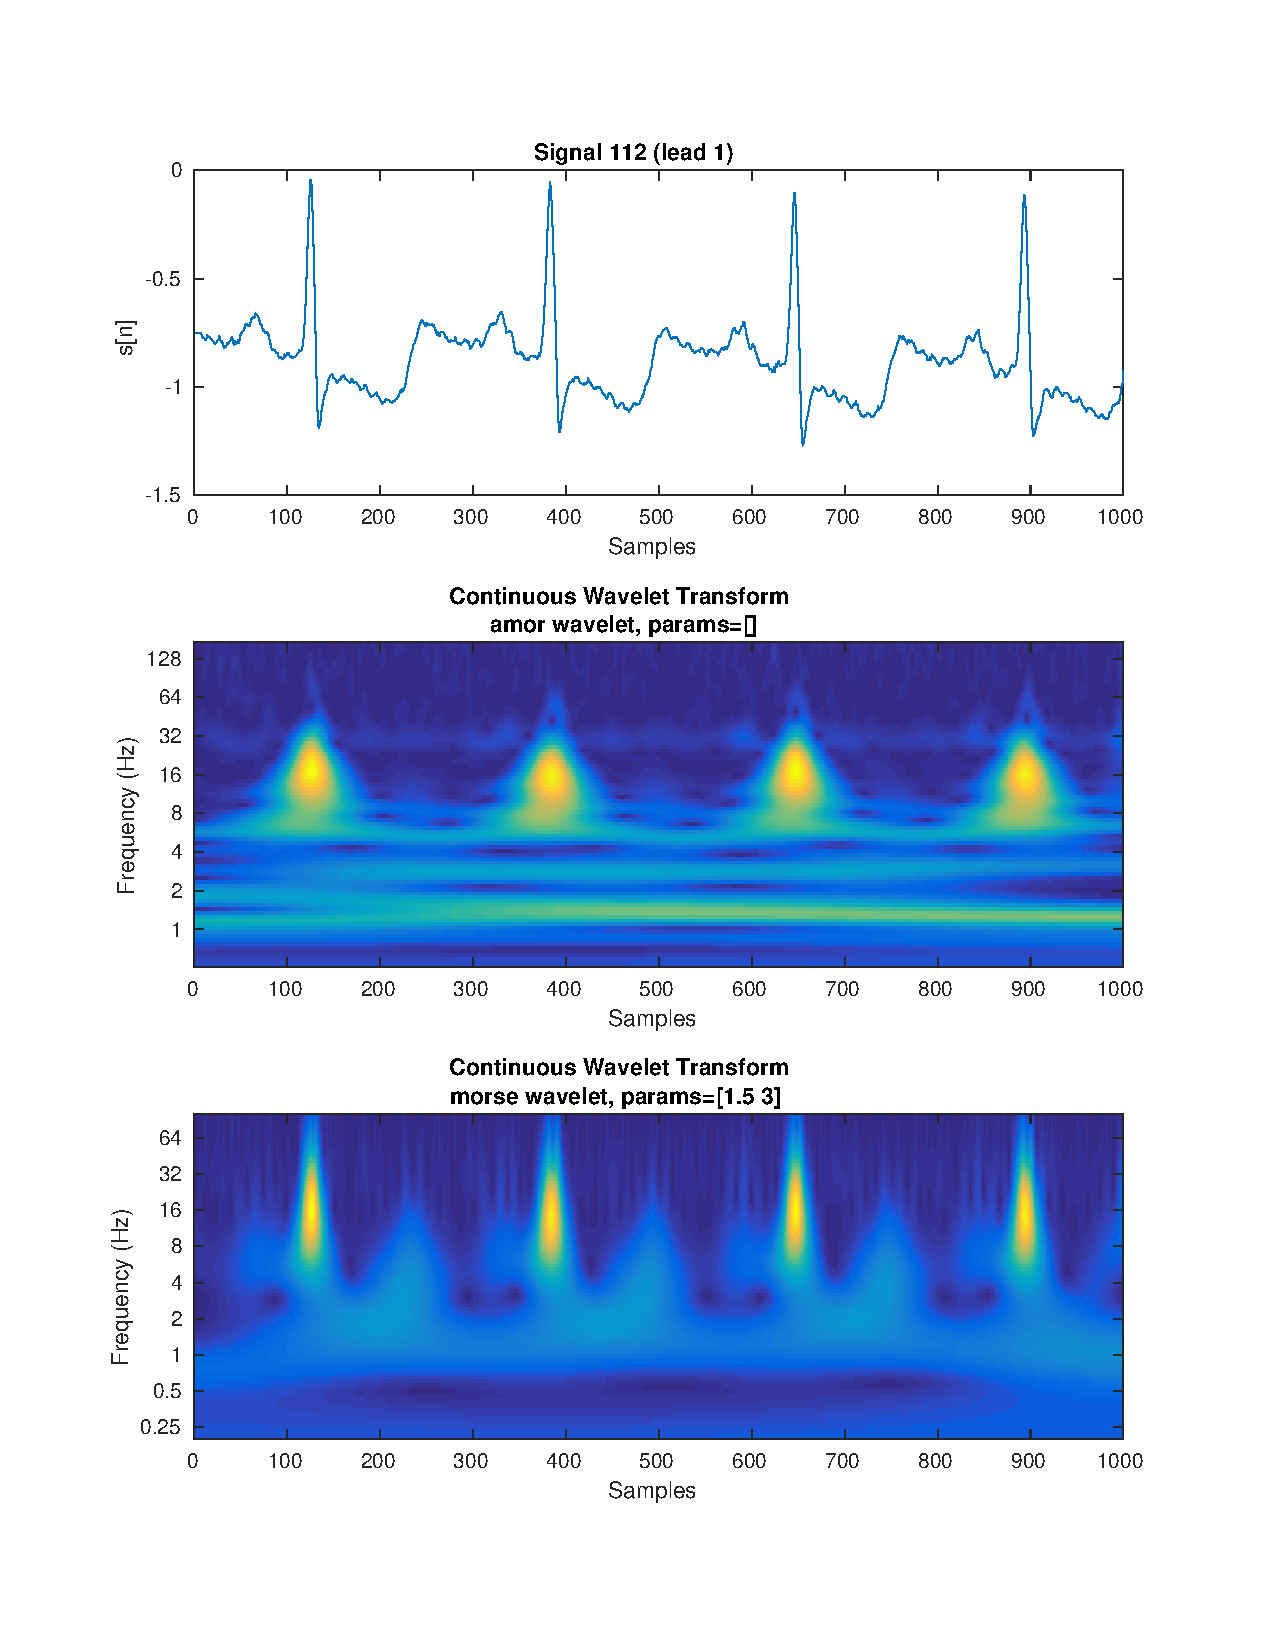
\includegraphics[width=\textwidth]{fig/112l1_cwt.pdf}
\end{figure}
\end{columns}
\end{frame}

\begin{frame}
\frametitle{Ανάλυση των σημάτων - 112 (Ακροδέκτης 1)}

\begin{columns}
\column{0.5\textwidth}
\begin{figure}
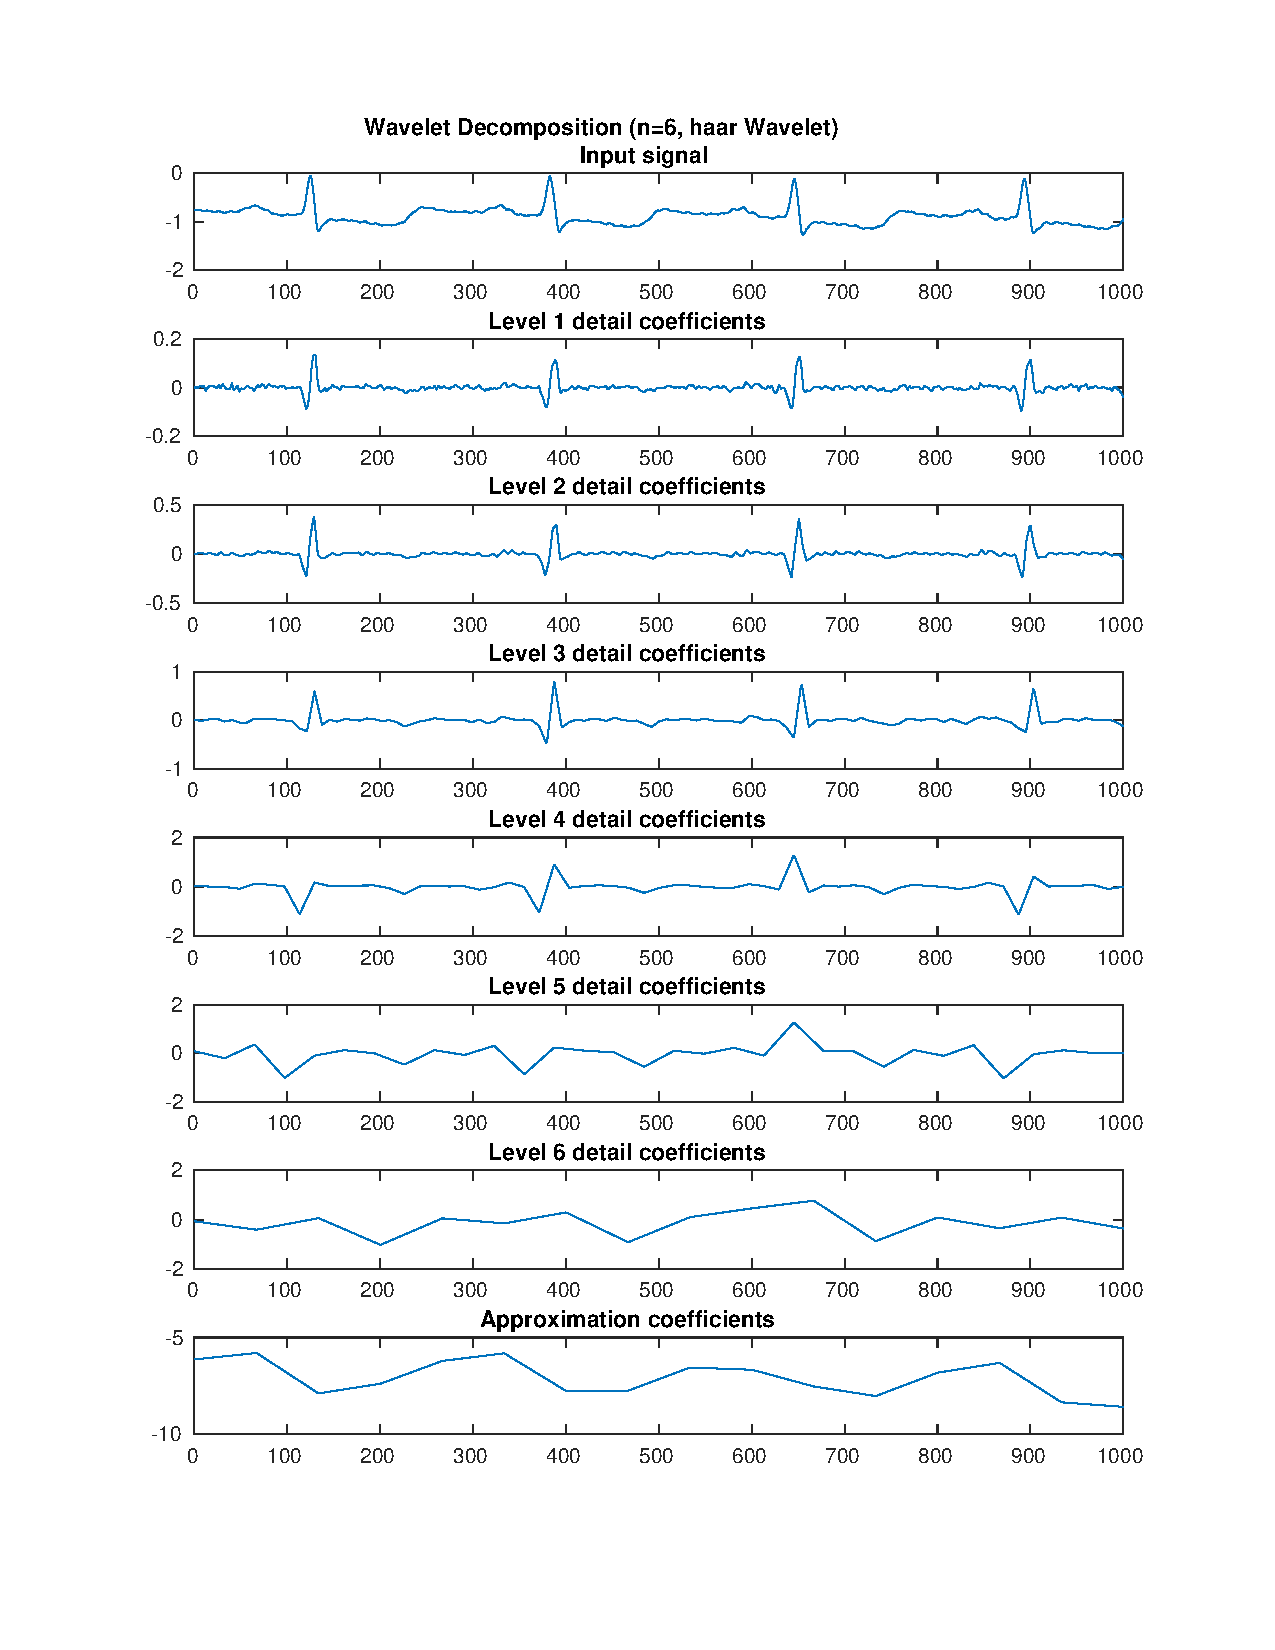
\includegraphics[width=\textwidth]{fig/112l1_dwt1.pdf}
\end{figure}

\column{0.5\textwidth}
\begin{figure}
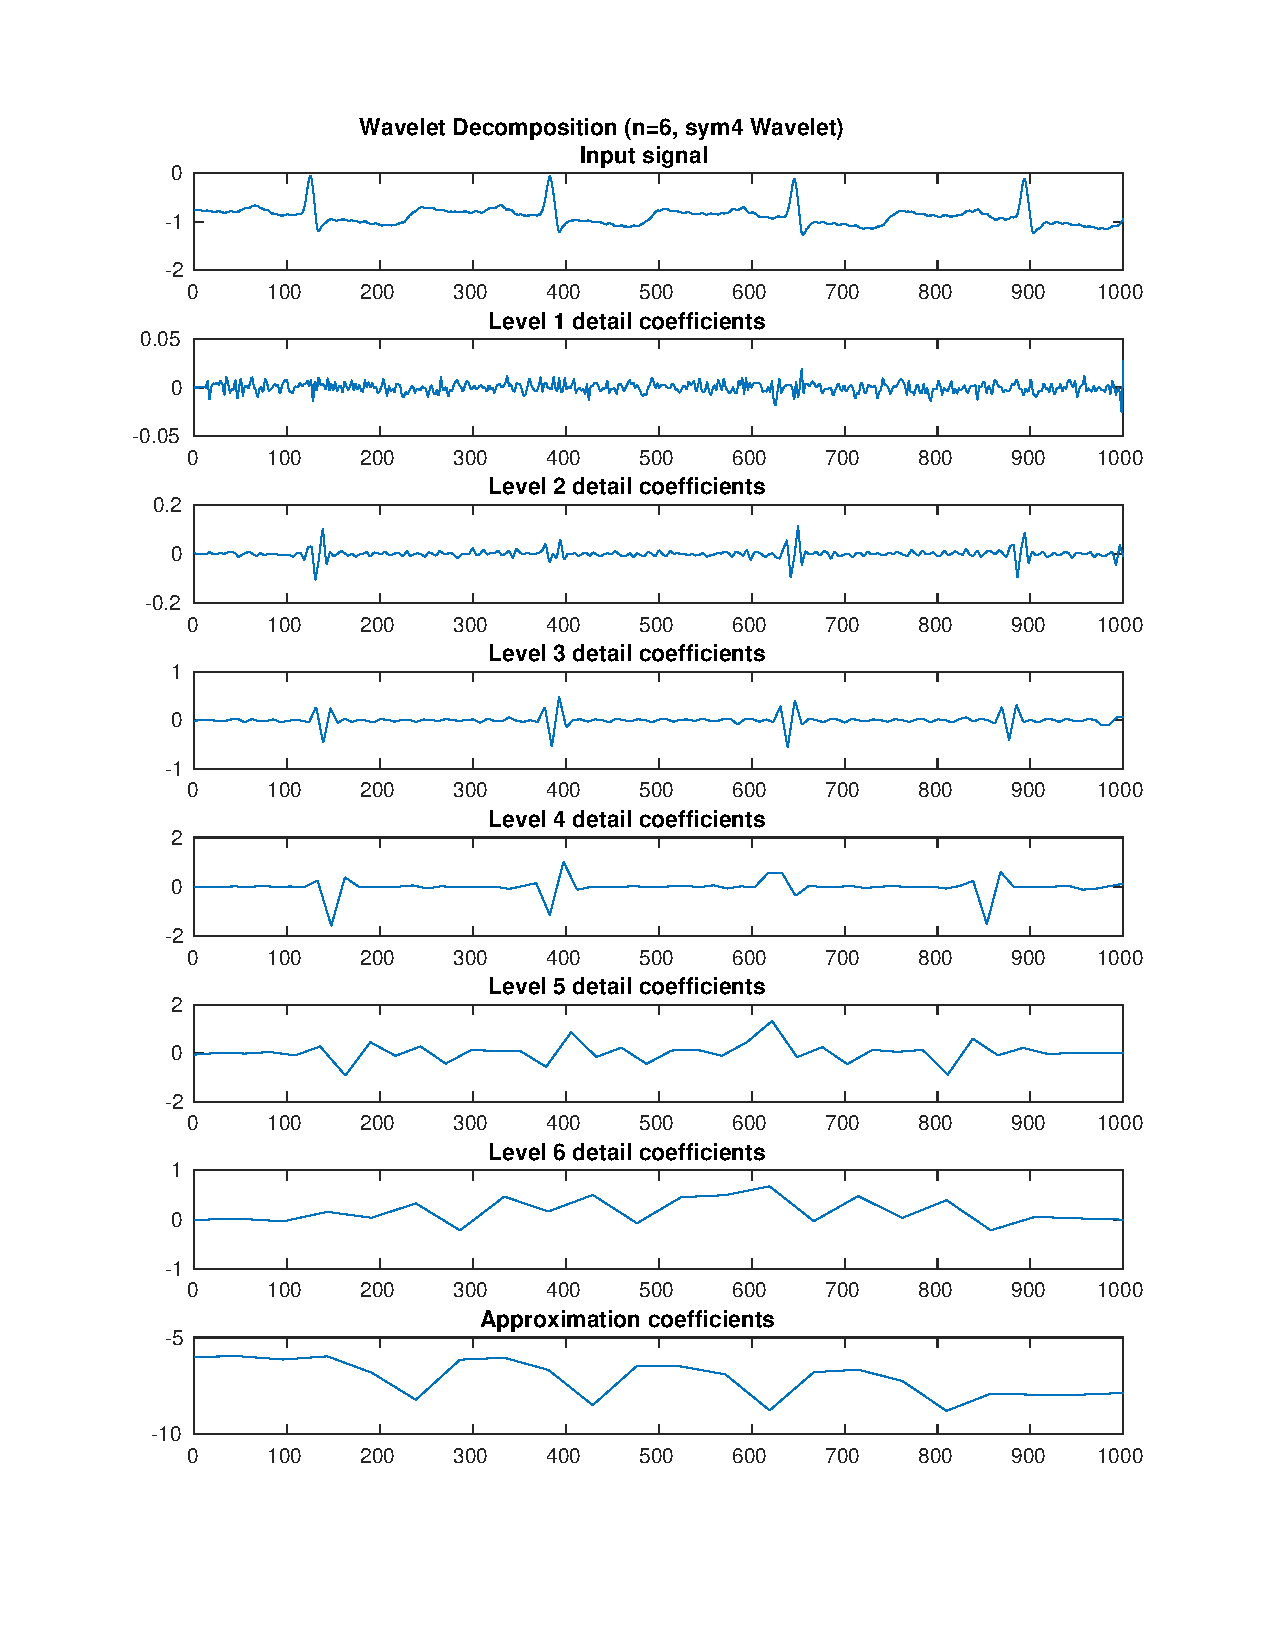
\includegraphics[width=\textwidth]{fig/112l1_dwt2.pdf}
\end{figure}
\end{columns}
\end{frame}

\begin{frame}
\frametitle{Ανάλυση των σημάτων - 112 (Ακροδέκτης 1)}

\begin{columns}
\column{0.5\textwidth}
\begin{figure}
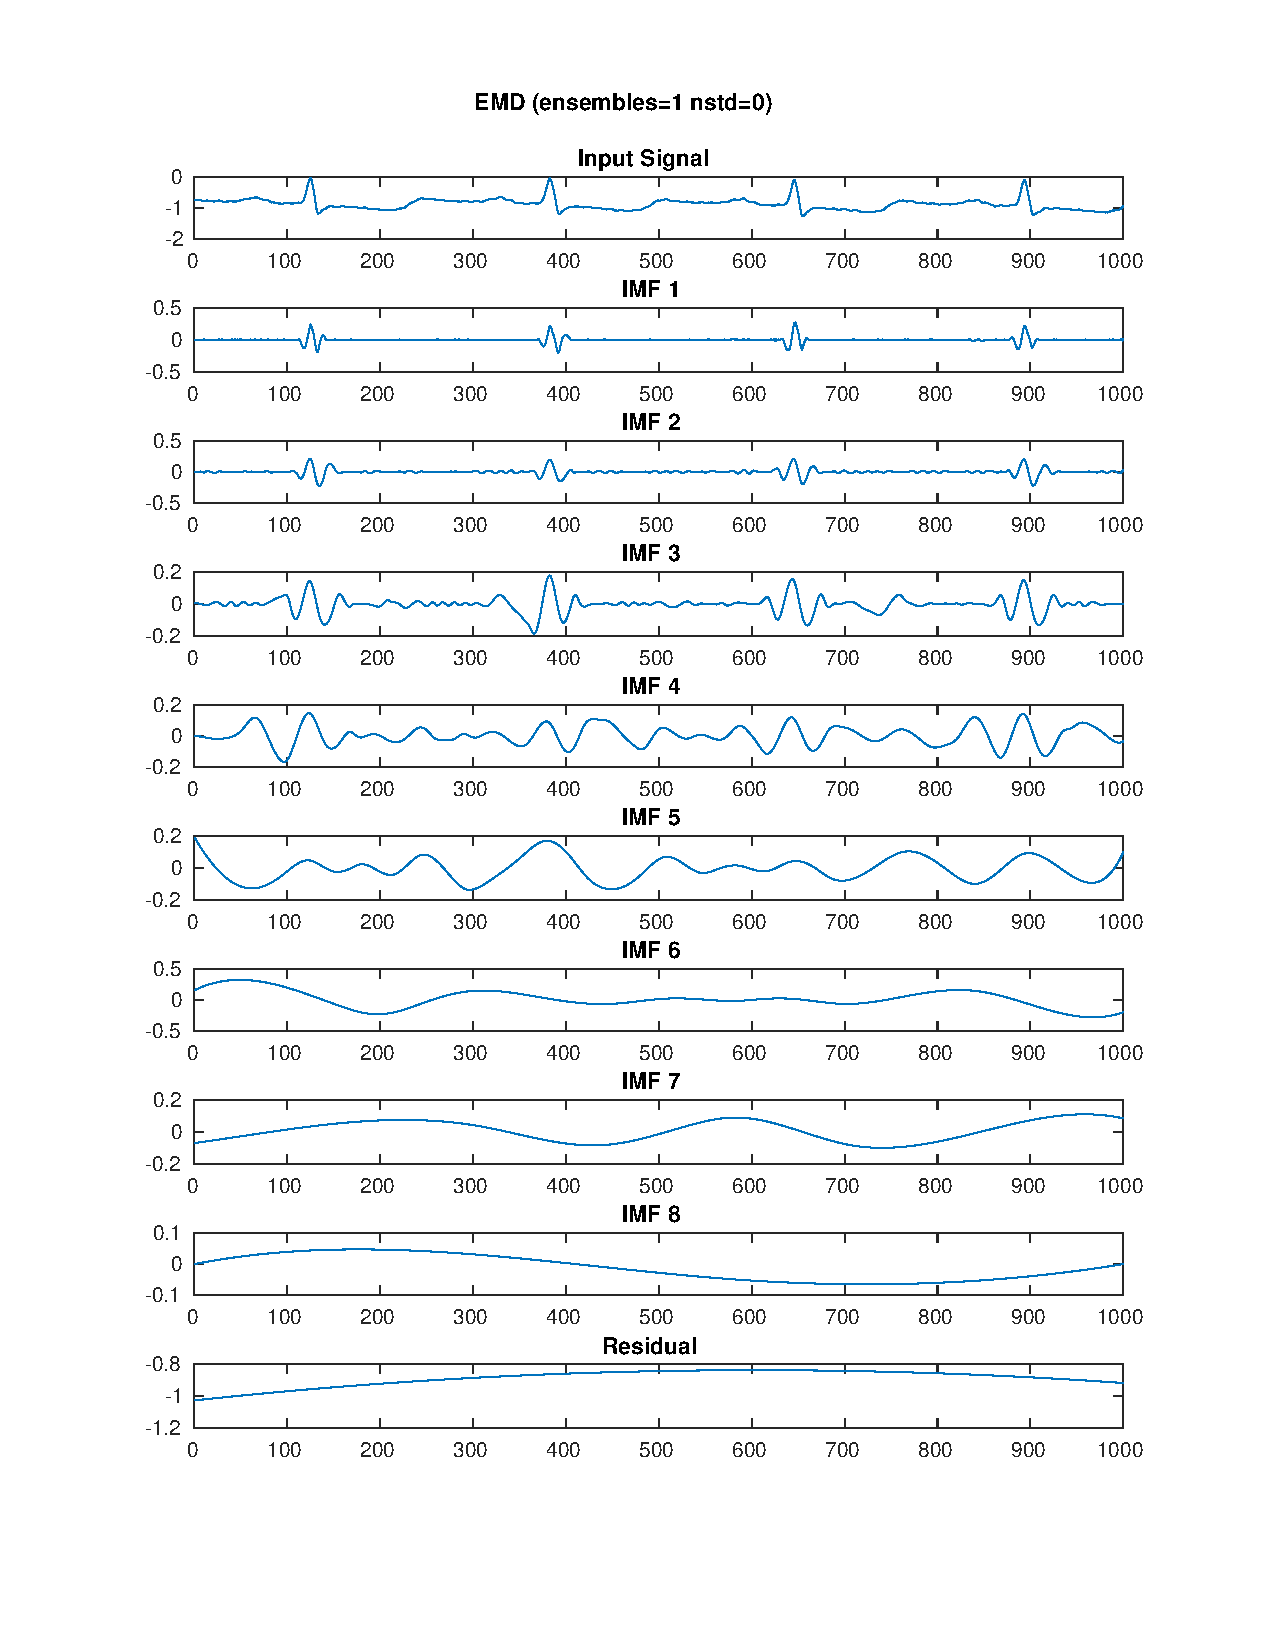
\includegraphics[width=\textwidth]{fig/112l1_emd.pdf}
\end{figure}

\column{0.5\textwidth}
\begin{figure}
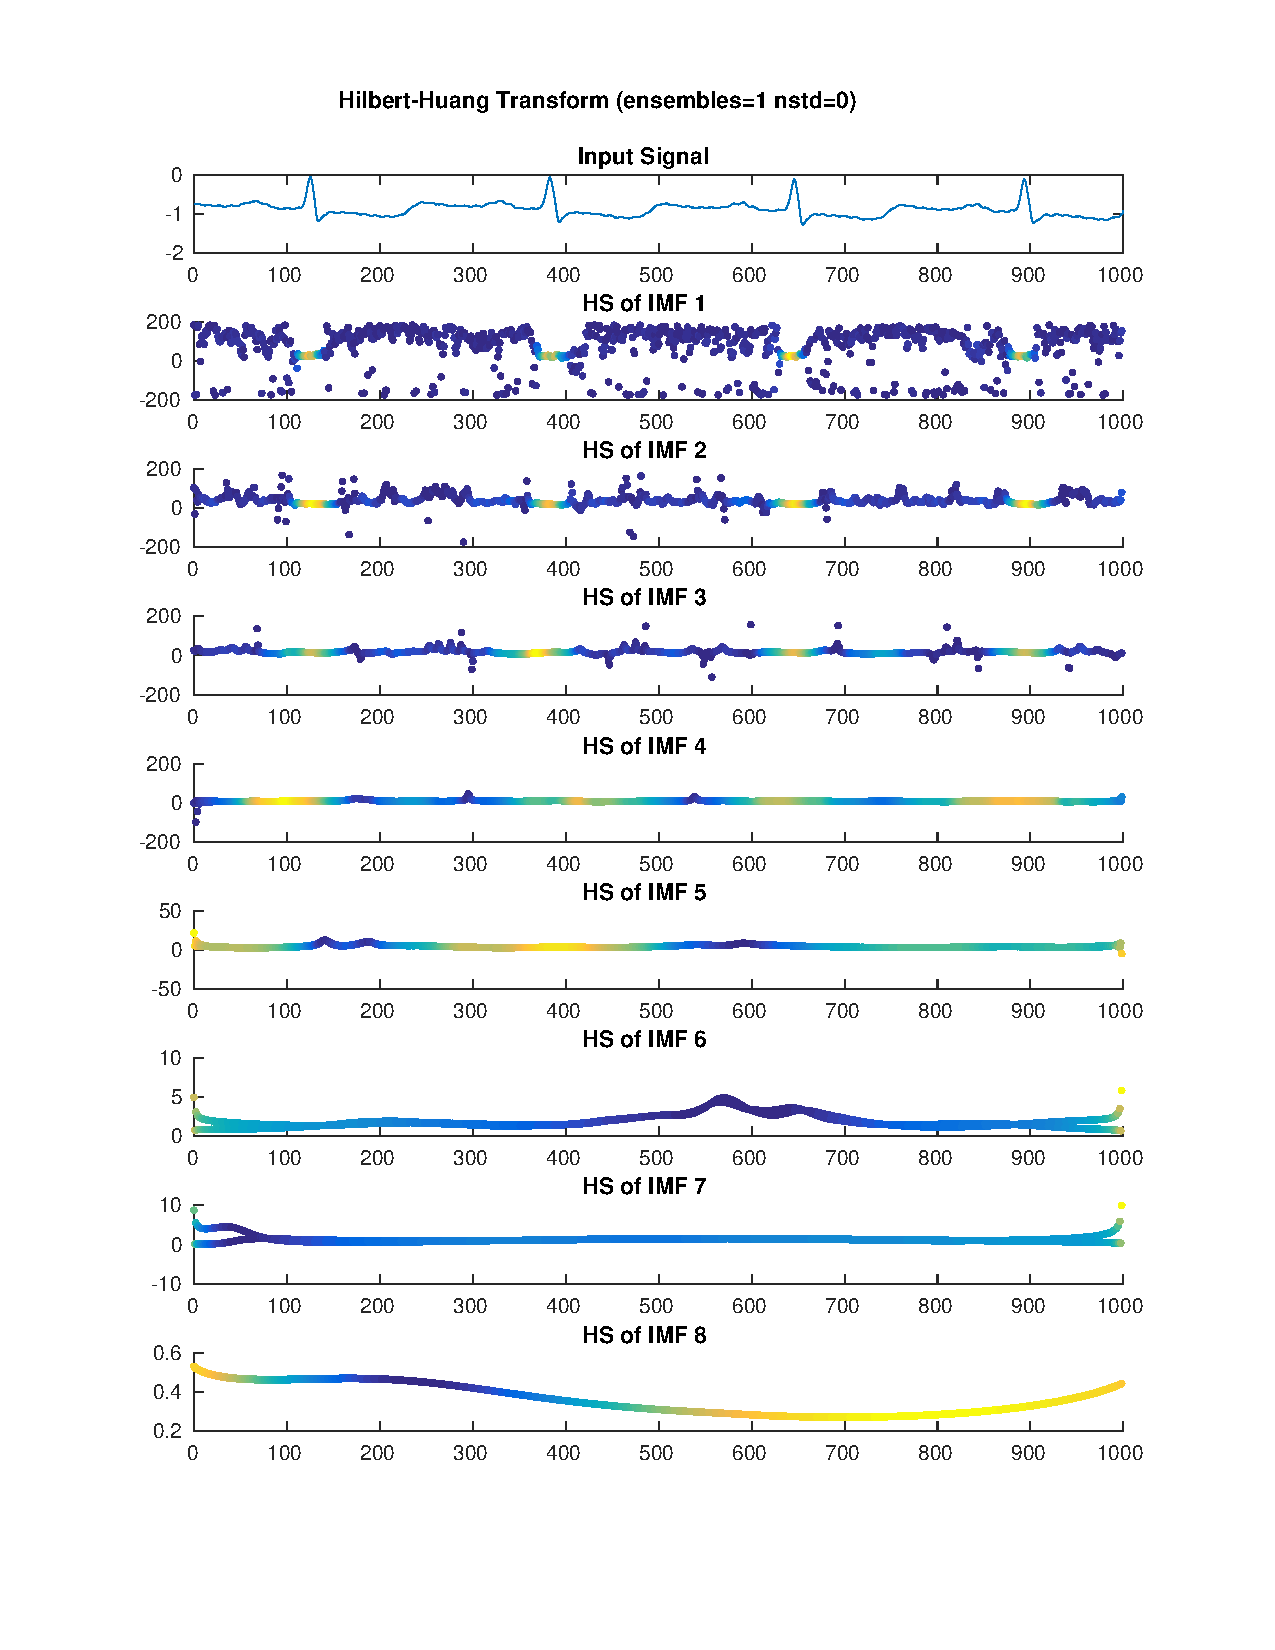
\includegraphics[width=\textwidth]{fig/112l1_hht.pdf}
\end{figure}
\end{columns}
\end{frame}

\begin{frame}
\frametitle{Ανάλυση των σημάτων - 112 (Ακροδέκτης 1)}

\begin{columns}
\column{0.5\textwidth}
\begin{figure}
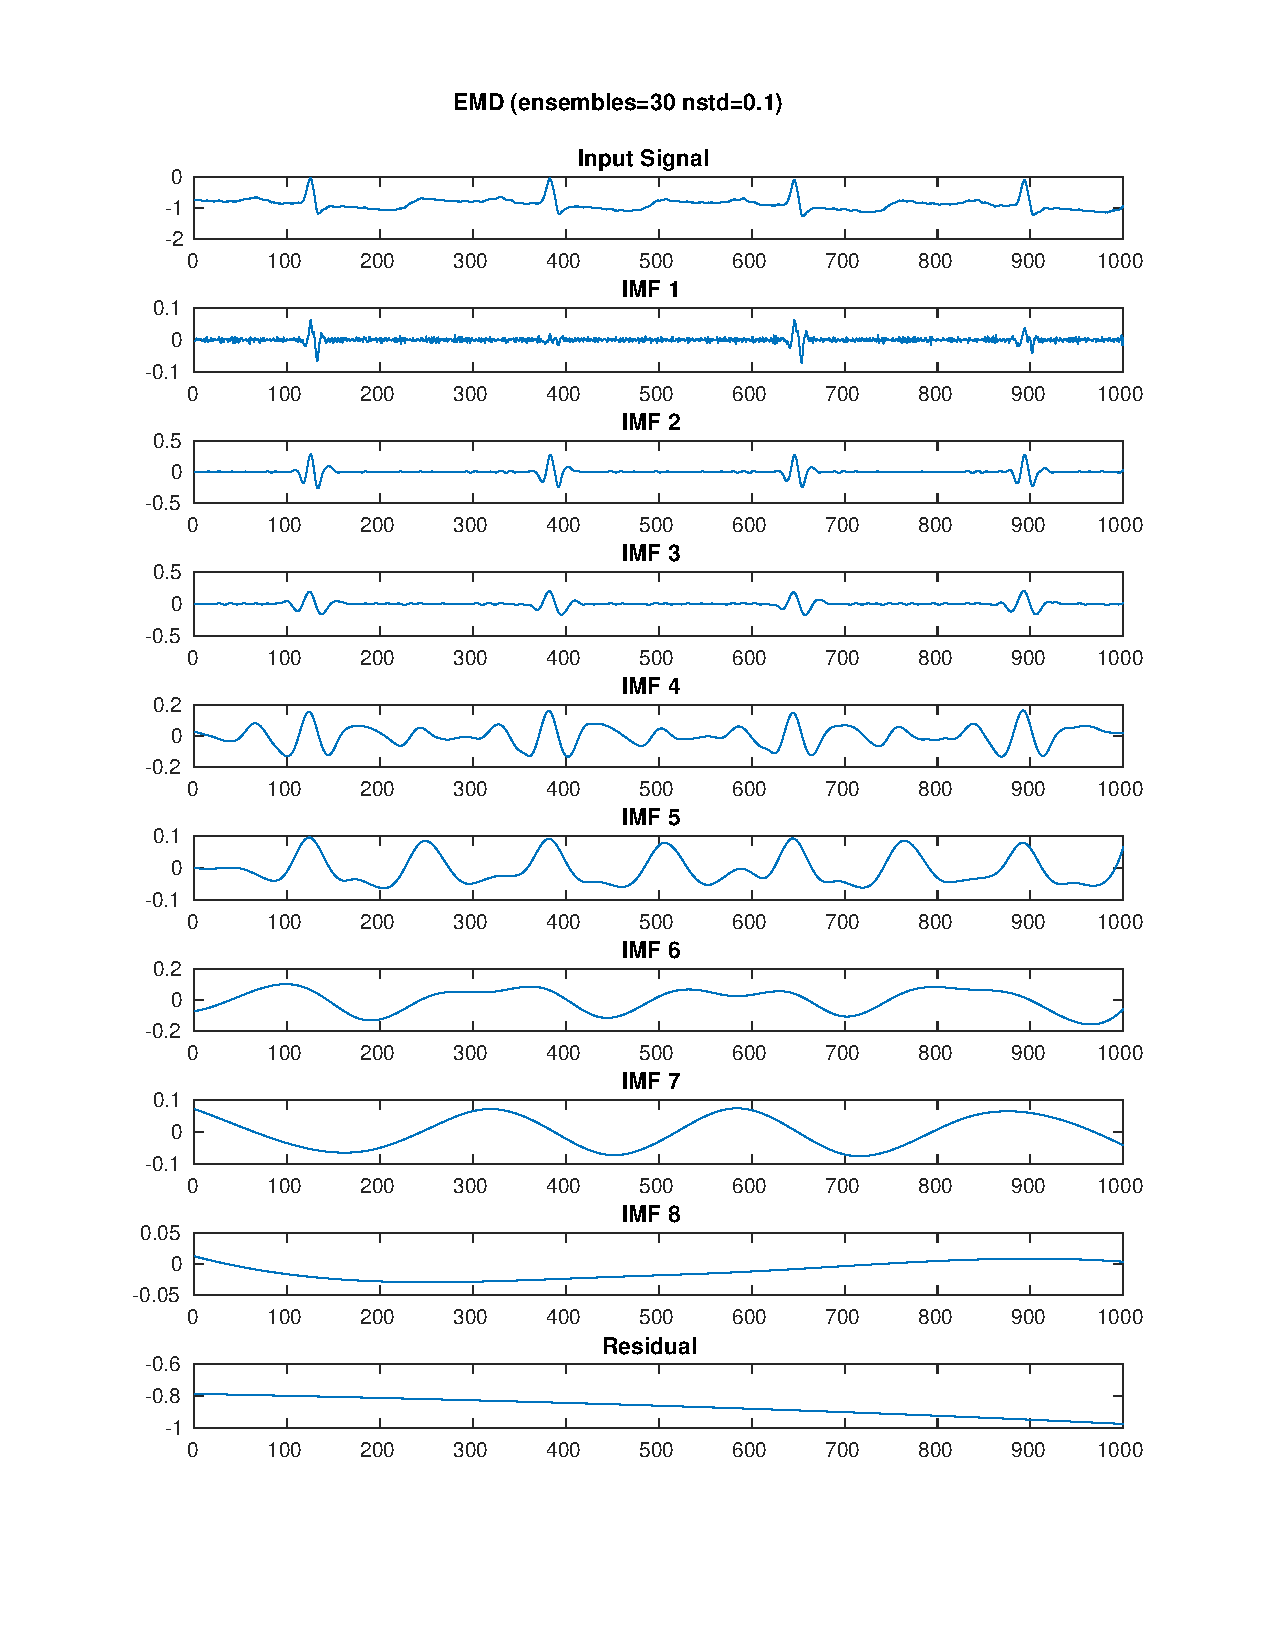
\includegraphics[width=\textwidth]{fig/112l1_emd_ensemble.pdf}
\end{figure}

\column{0.5\textwidth}
\begin{figure}
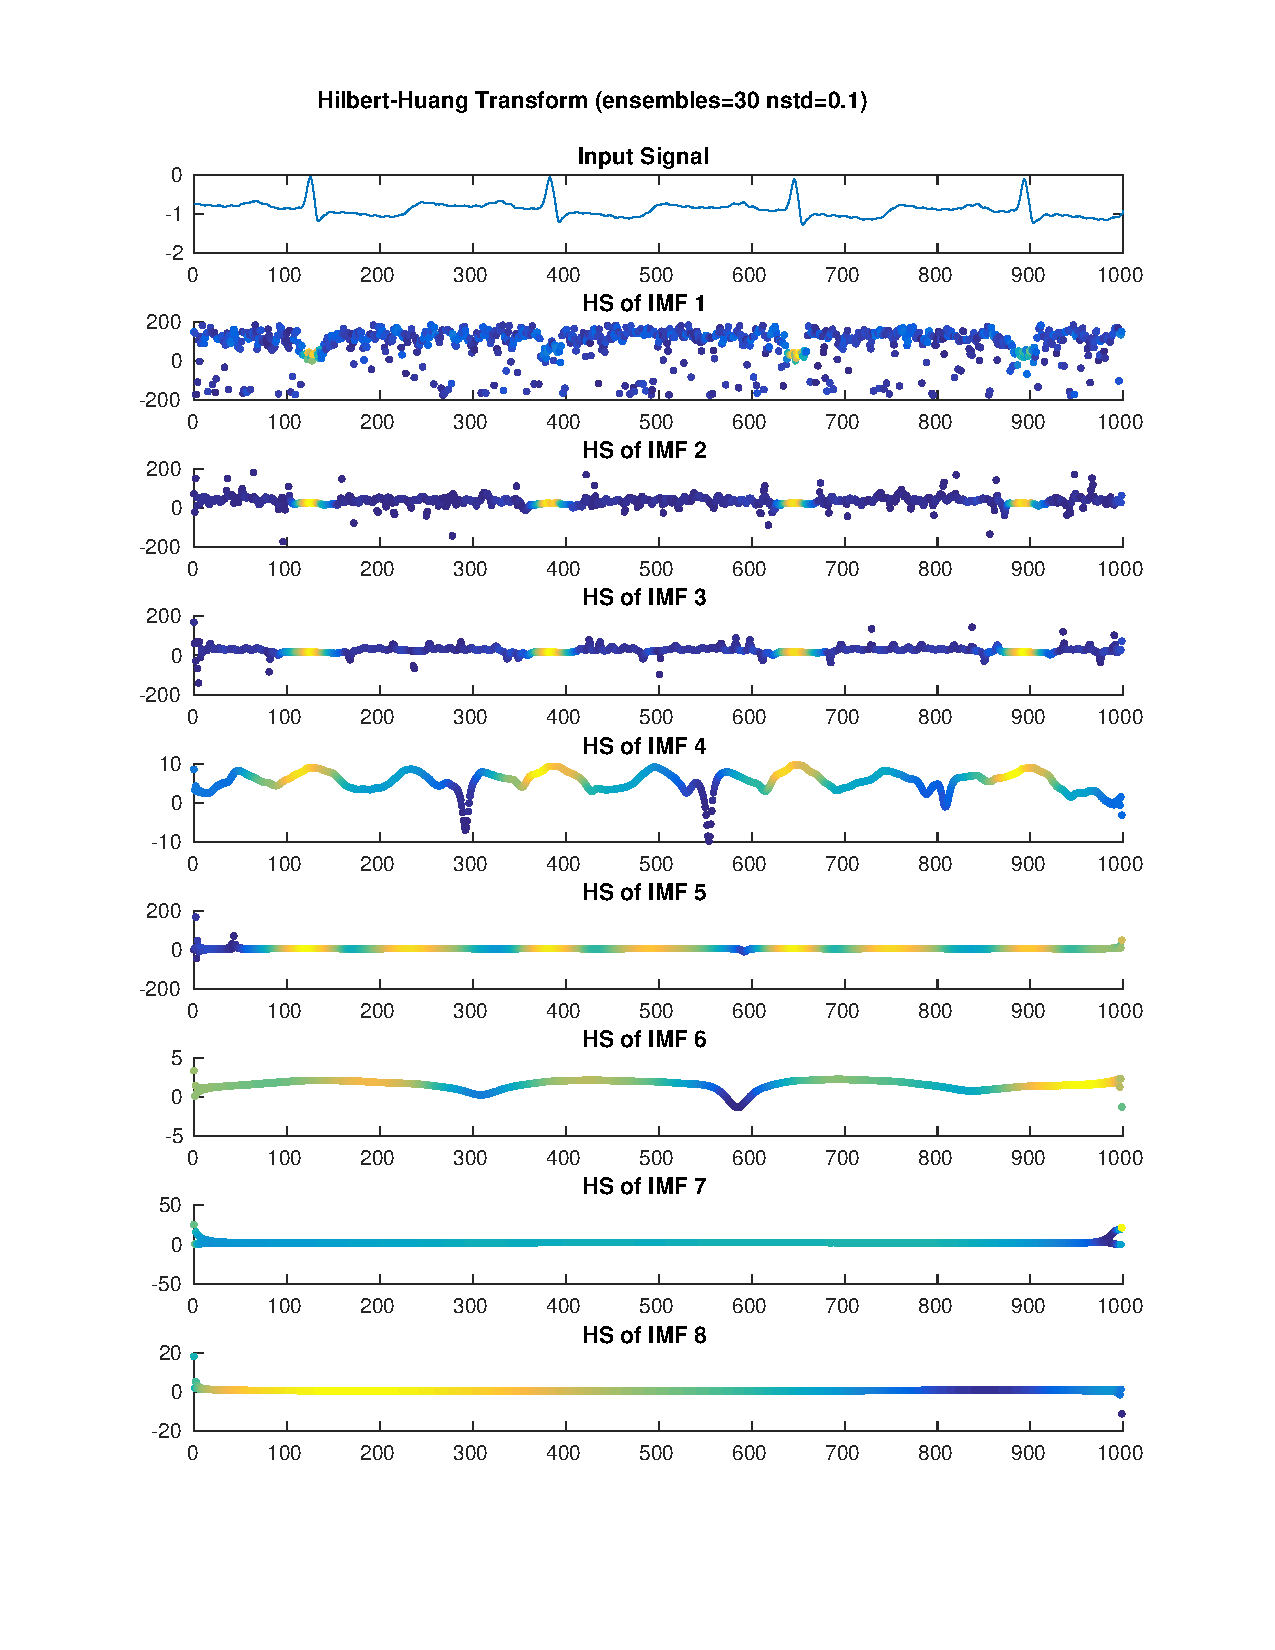
\includegraphics[width=\textwidth]{fig/112l1_hht_ensemble.pdf}
\end{figure}
\end{columns}
\end{frame}


% --- Ανάλυση 112 (lead 2) ---
\subsection{Σήμα 112 (Ακροδέκτης 2)}
\label{sig:112l2}
\begin{frame}
\frametitle{Ανάλυση των σημάτων - 112 (Ακροδέκτης 2)}

\begin{columns}
\column{0.5\textwidth}
\begin{figure}
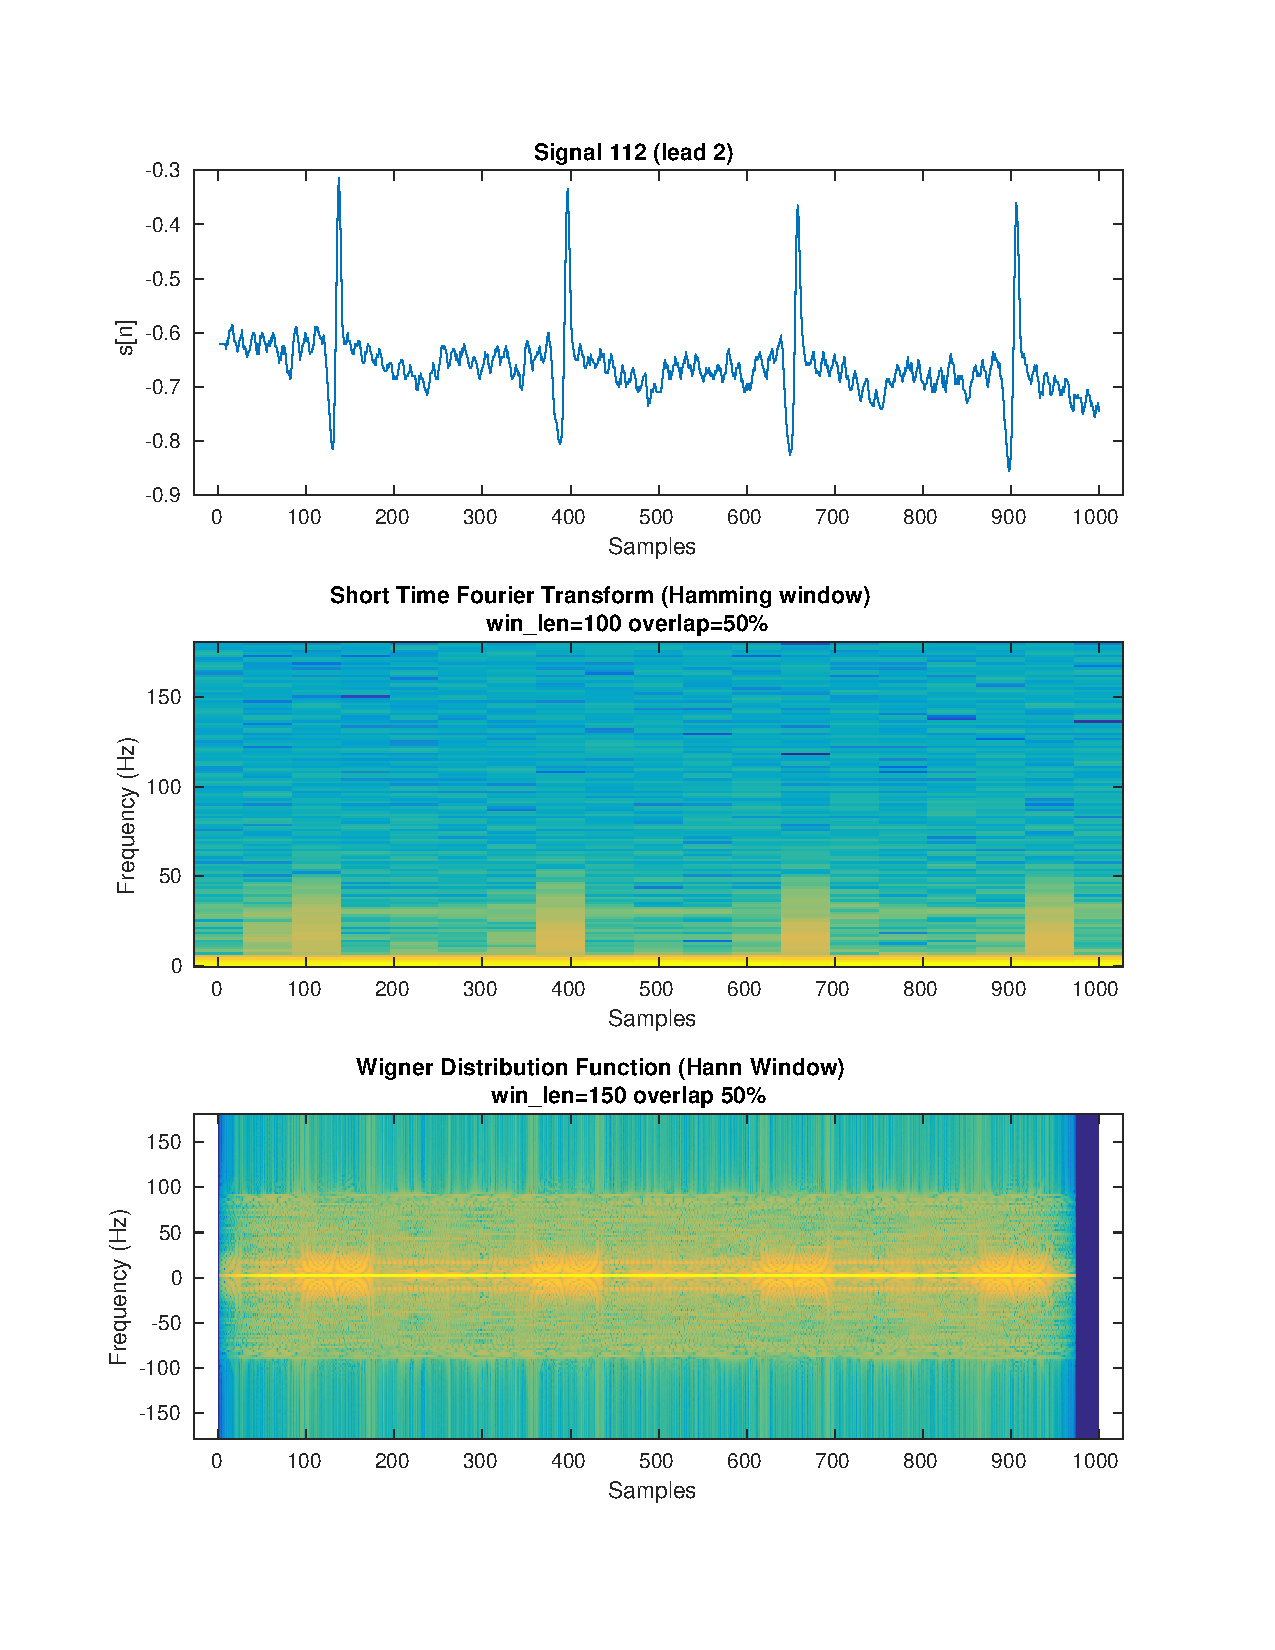
\includegraphics[width=\textwidth]{fig/112l2_stft_wdf.pdf}
\end{figure}

\column{0.5\textwidth}
\begin{figure}
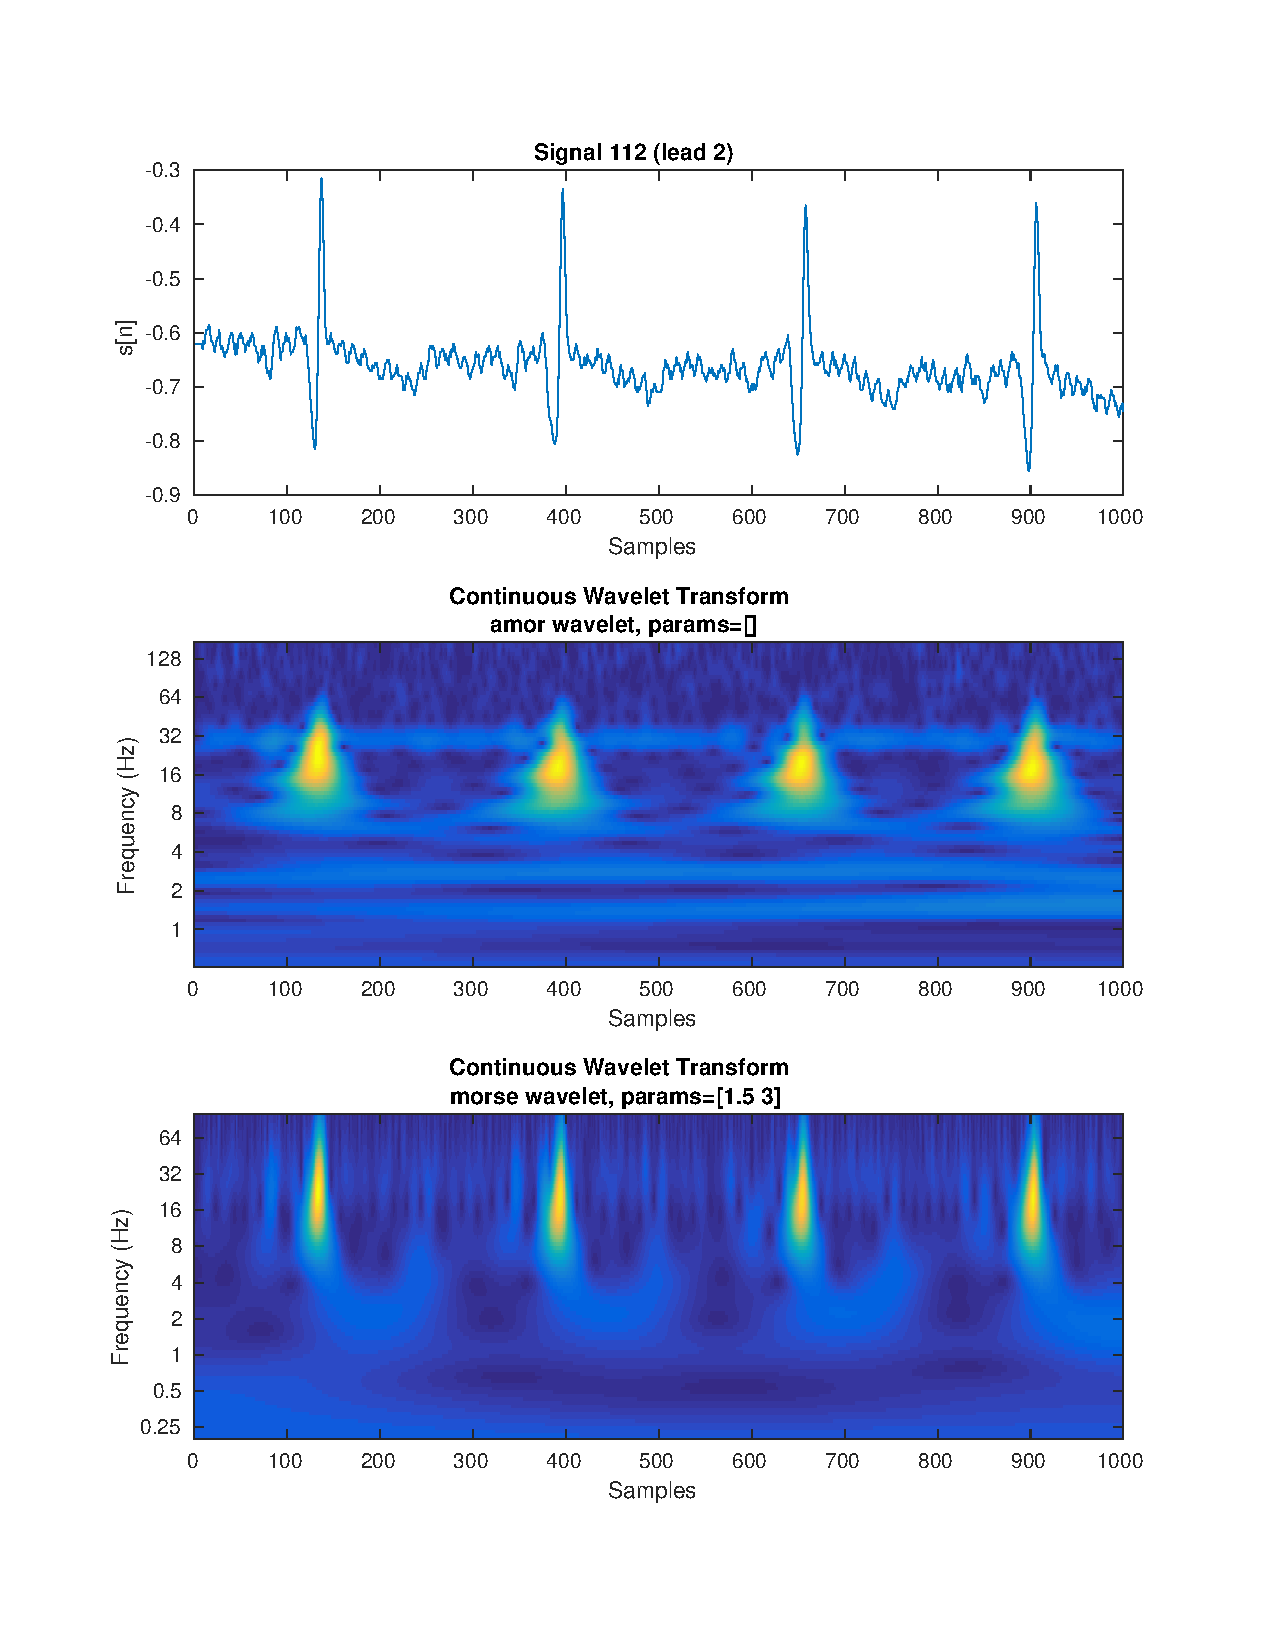
\includegraphics[width=\textwidth]{fig/112l2_cwt.pdf}
\end{figure}
\end{columns}
\end{frame}

\begin{frame}
\frametitle{Ανάλυση των σημάτων - 112 (Ακροδέκτης 2)}

\begin{columns}
\column{0.5\textwidth}
\begin{figure}
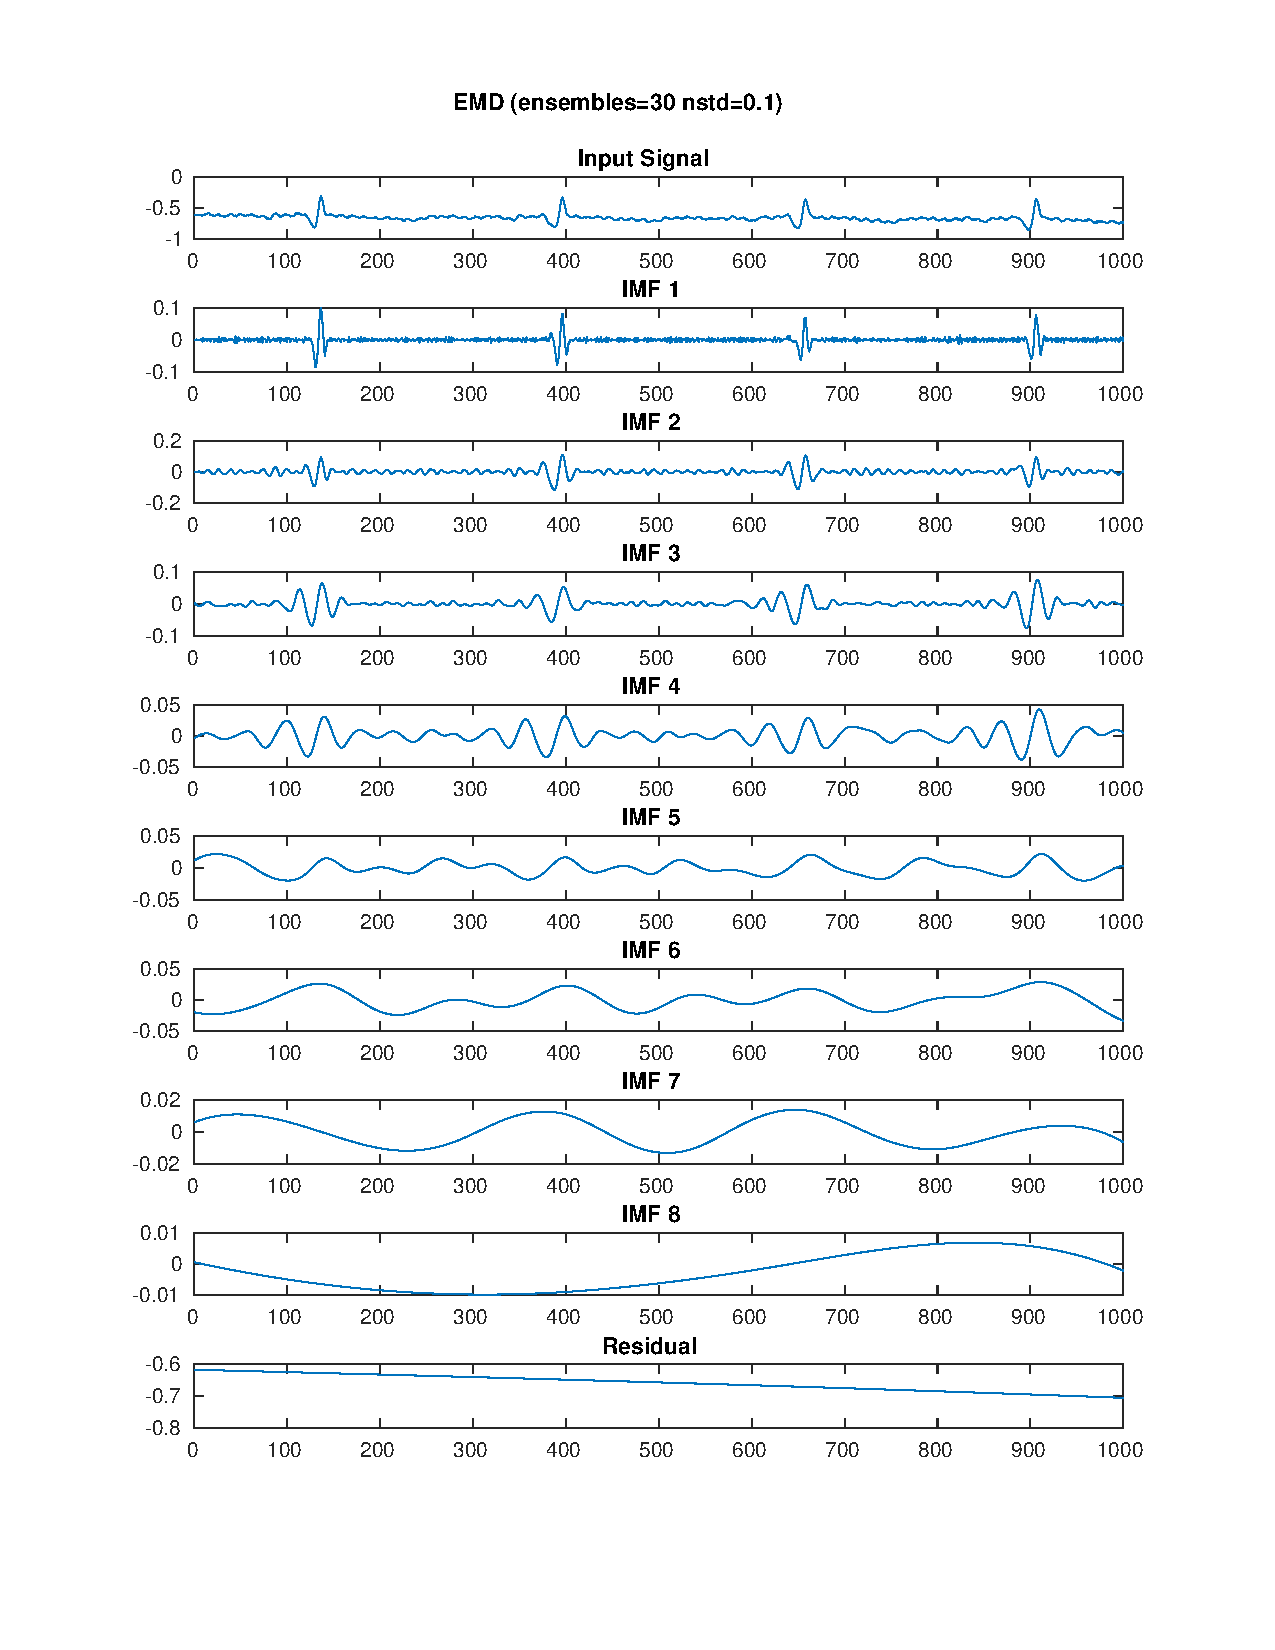
\includegraphics[width=\textwidth]{fig/112l2_emd_ensemble.pdf}
\end{figure}

\column{0.5\textwidth}
\begin{figure}
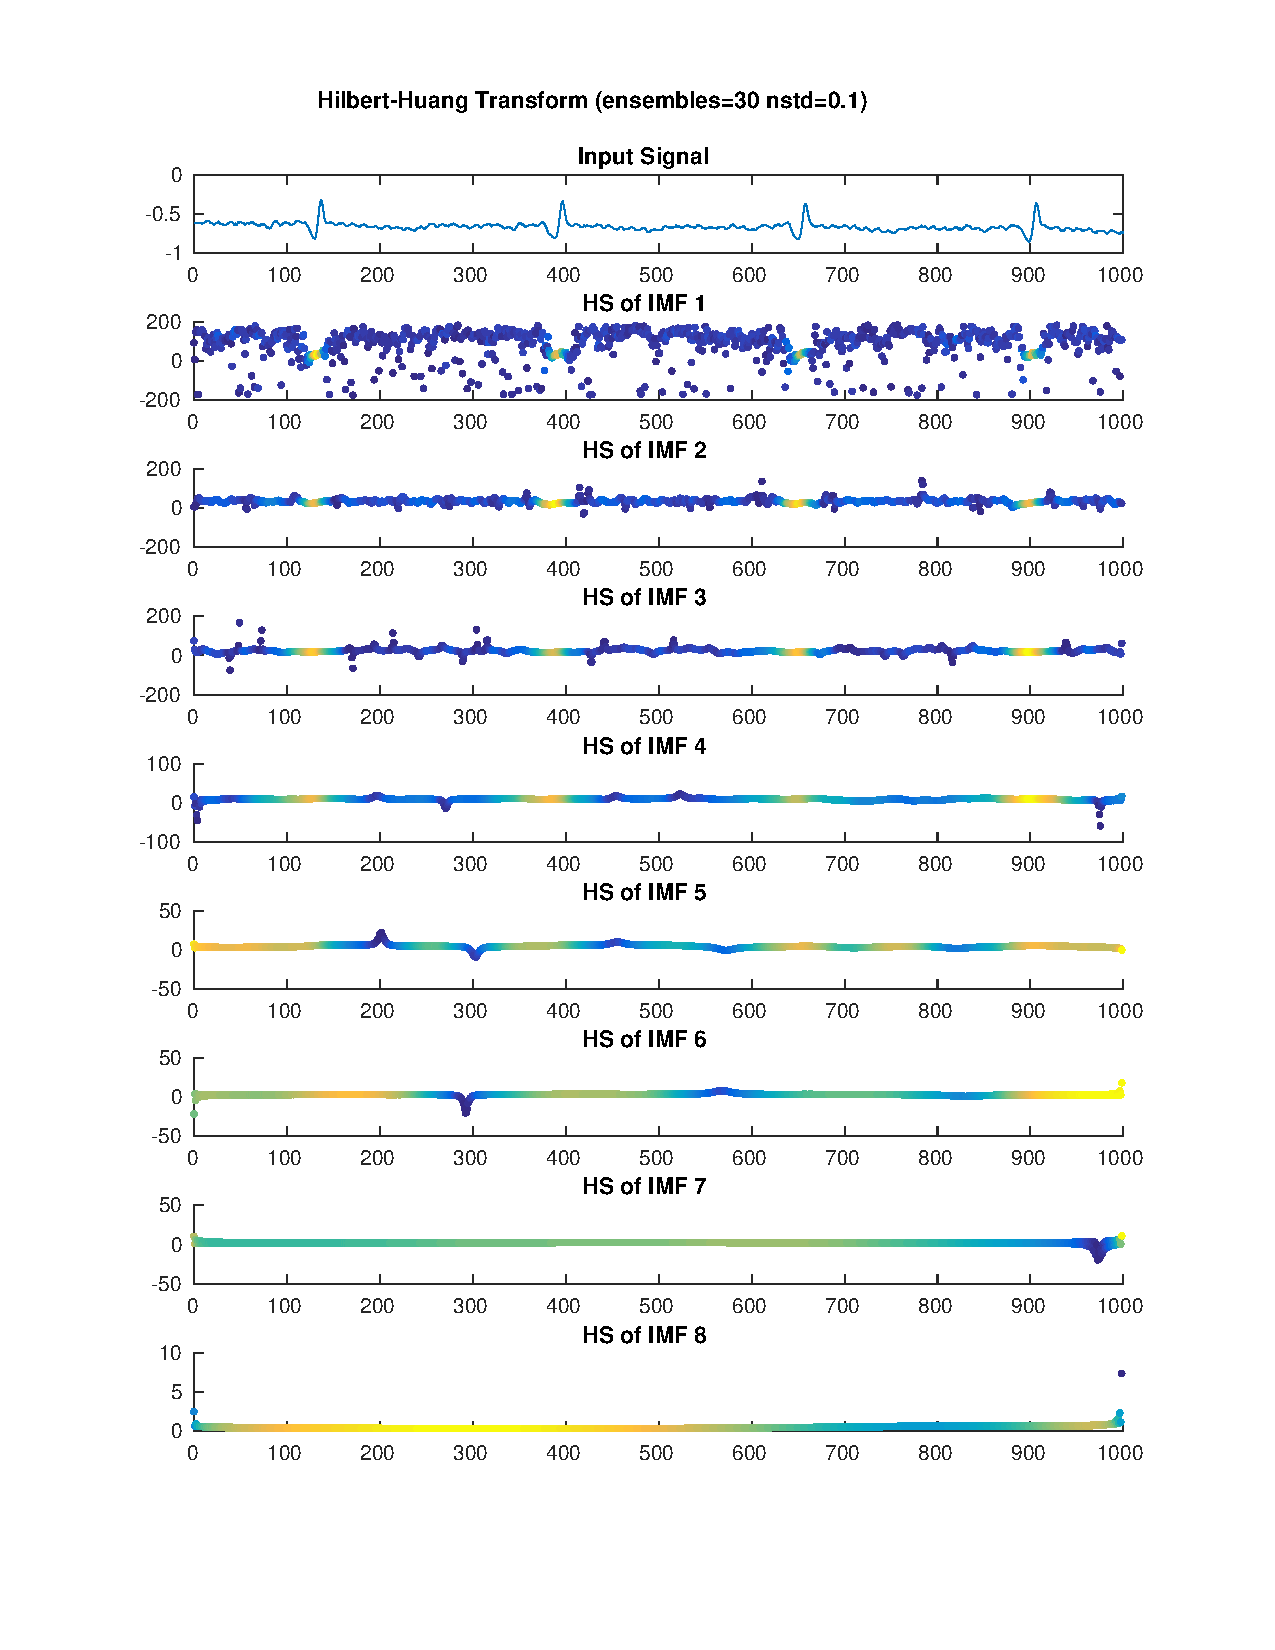
\includegraphics[width=\textwidth]{fig/112l2_hht_ensemble.pdf}
\end{figure}
\end{columns}
\end{frame}


% --- Ανάλυση 123 ---
\subsection{Σήμα 123}
\label{sig:123}
\begin{frame}
\frametitle{Ανάλυση των σημάτων - 123}

\begin{columns}
\column{0.5\textwidth}
\begin{figure}
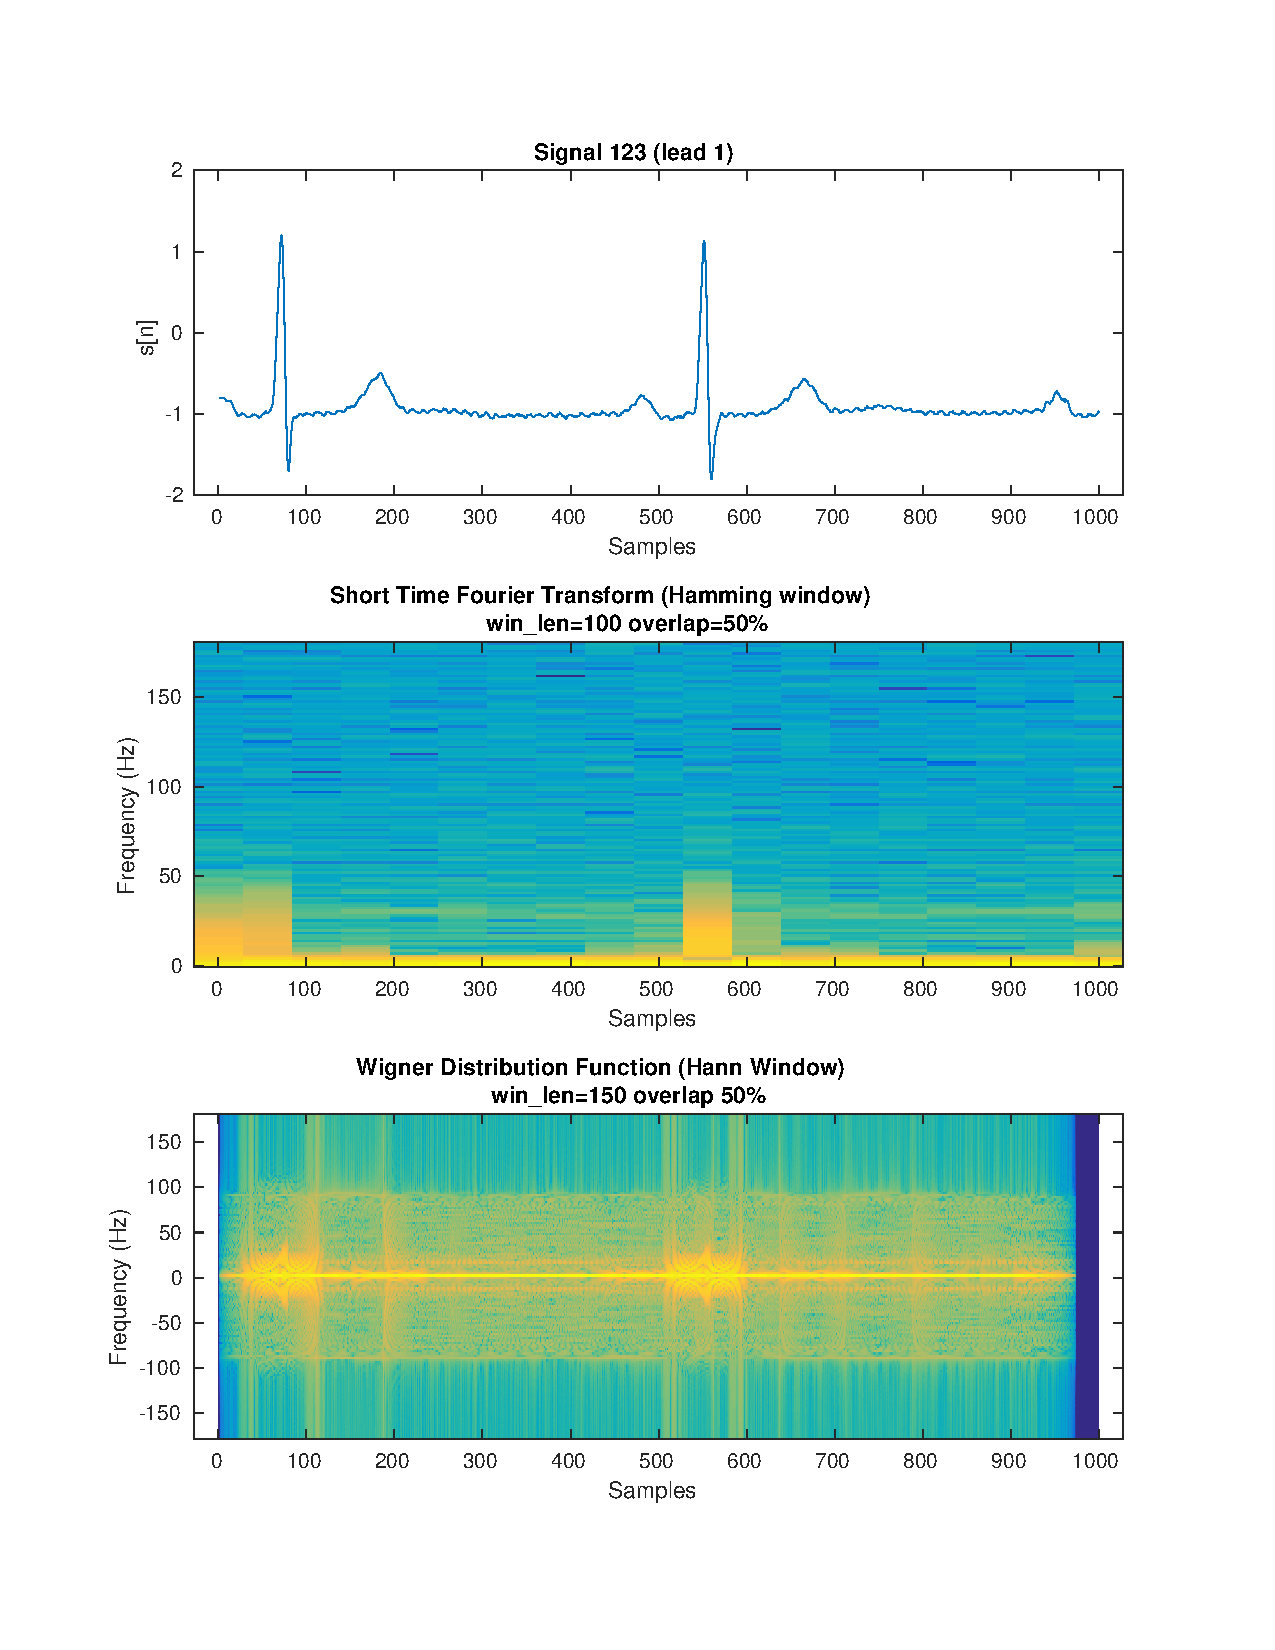
\includegraphics[width=\textwidth]{fig/123l1_stft_wdf.pdf}
\end{figure}

\column{0.5\textwidth}
\begin{figure}
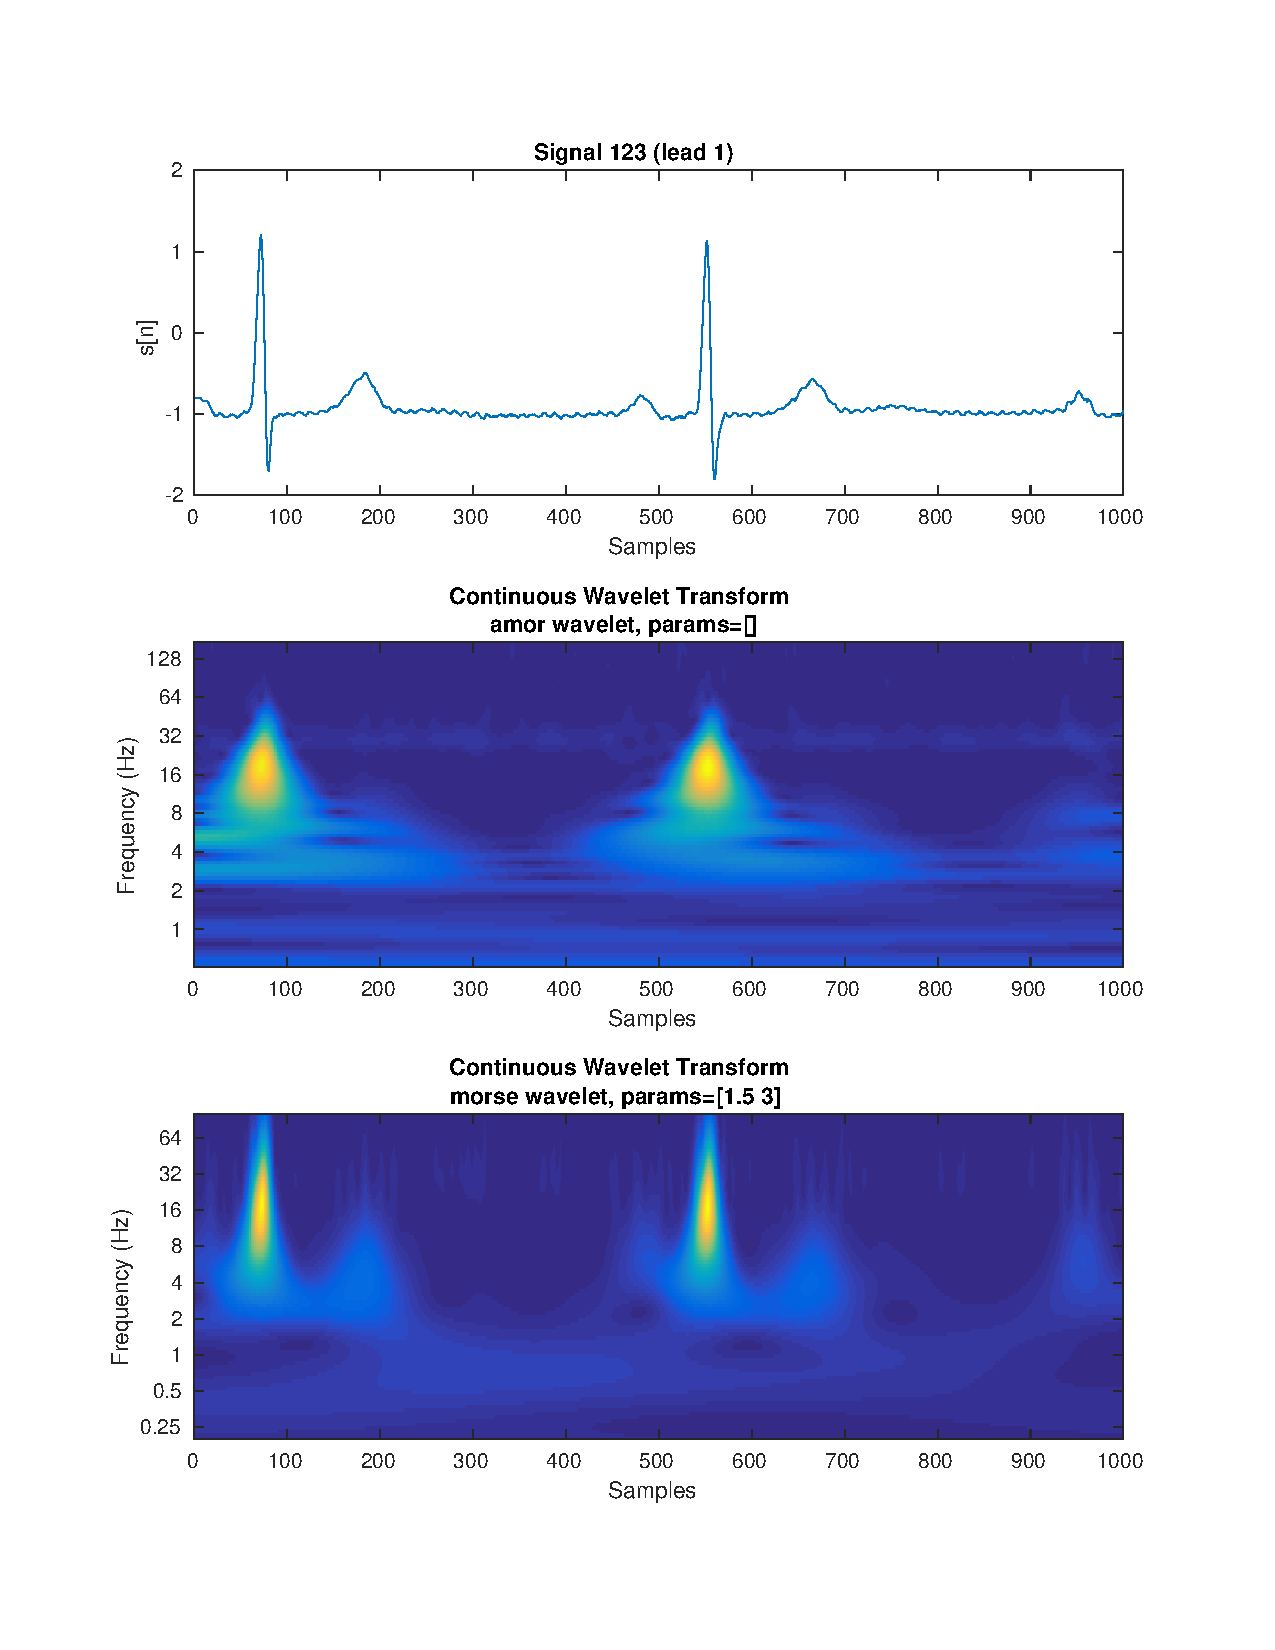
\includegraphics[width=\textwidth]{fig/123l1_cwt.pdf}
\end{figure}
\end{columns}
\end{frame}

\begin{frame}
\frametitle{Ανάλυση των σημάτων - 123}

\begin{columns}
\column{0.5\textwidth}
\begin{figure}
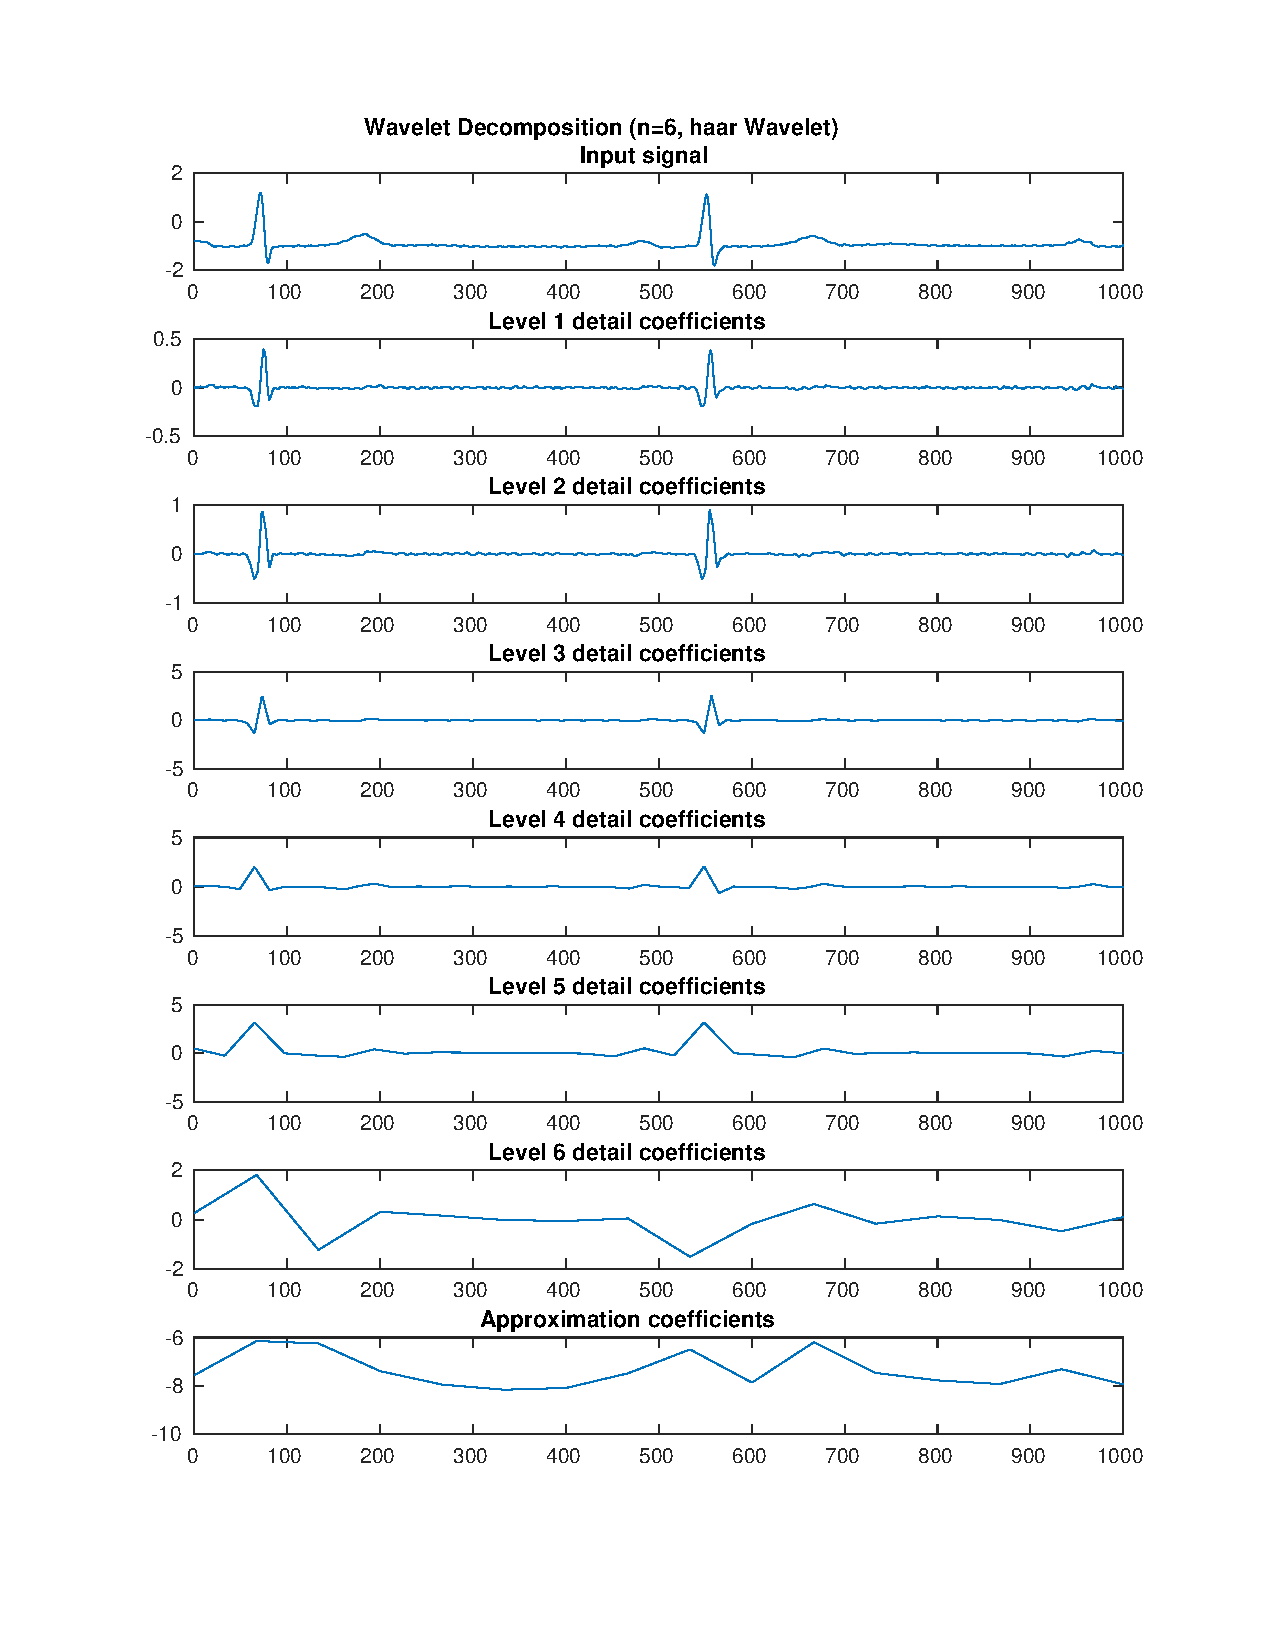
\includegraphics[width=\textwidth]{fig/123l1_dwt1.pdf}
\end{figure}

\column{0.5\textwidth}
\begin{figure}
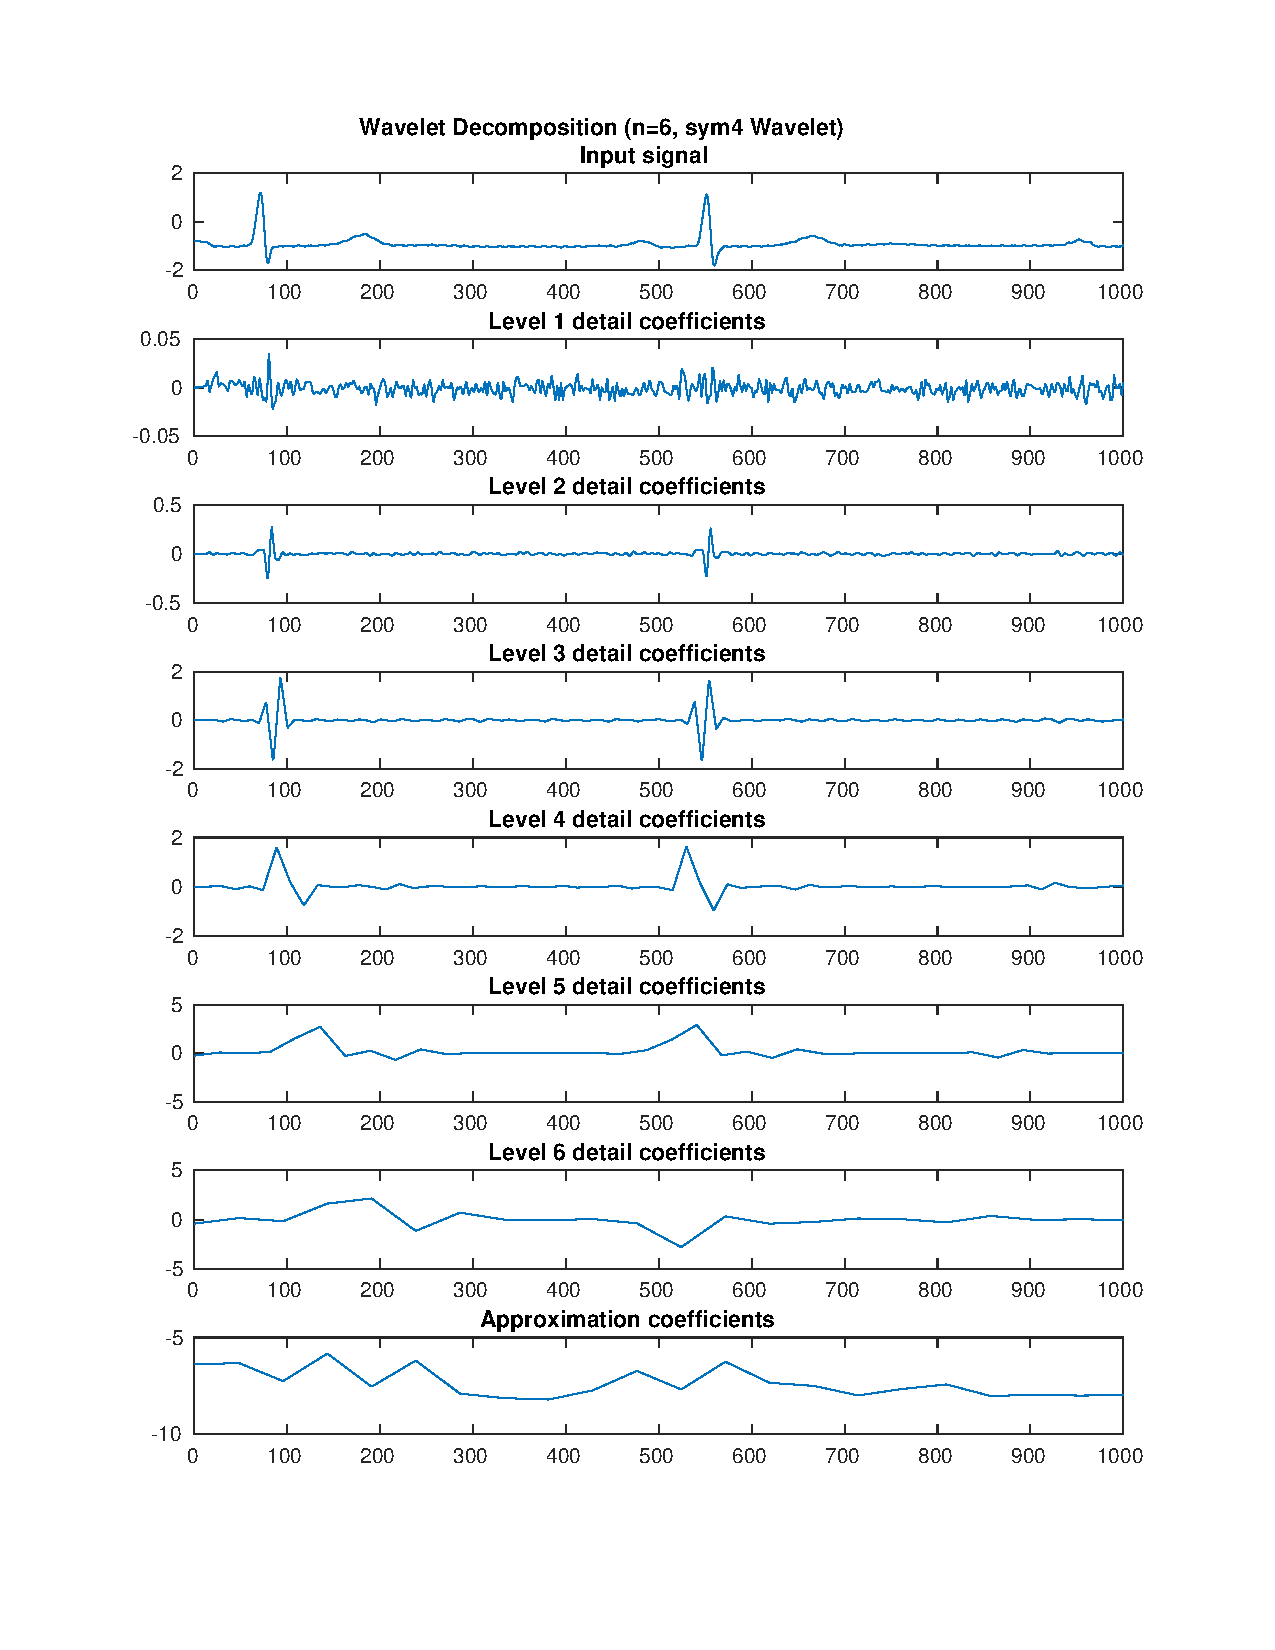
\includegraphics[width=\textwidth]{fig/123l1_dwt2.pdf}
\end{figure}
\end{columns}
\end{frame}

\begin{frame}
\frametitle{Ανάλυση των σημάτων - 123}

\begin{columns}
\column{0.5\textwidth}
\begin{figure}
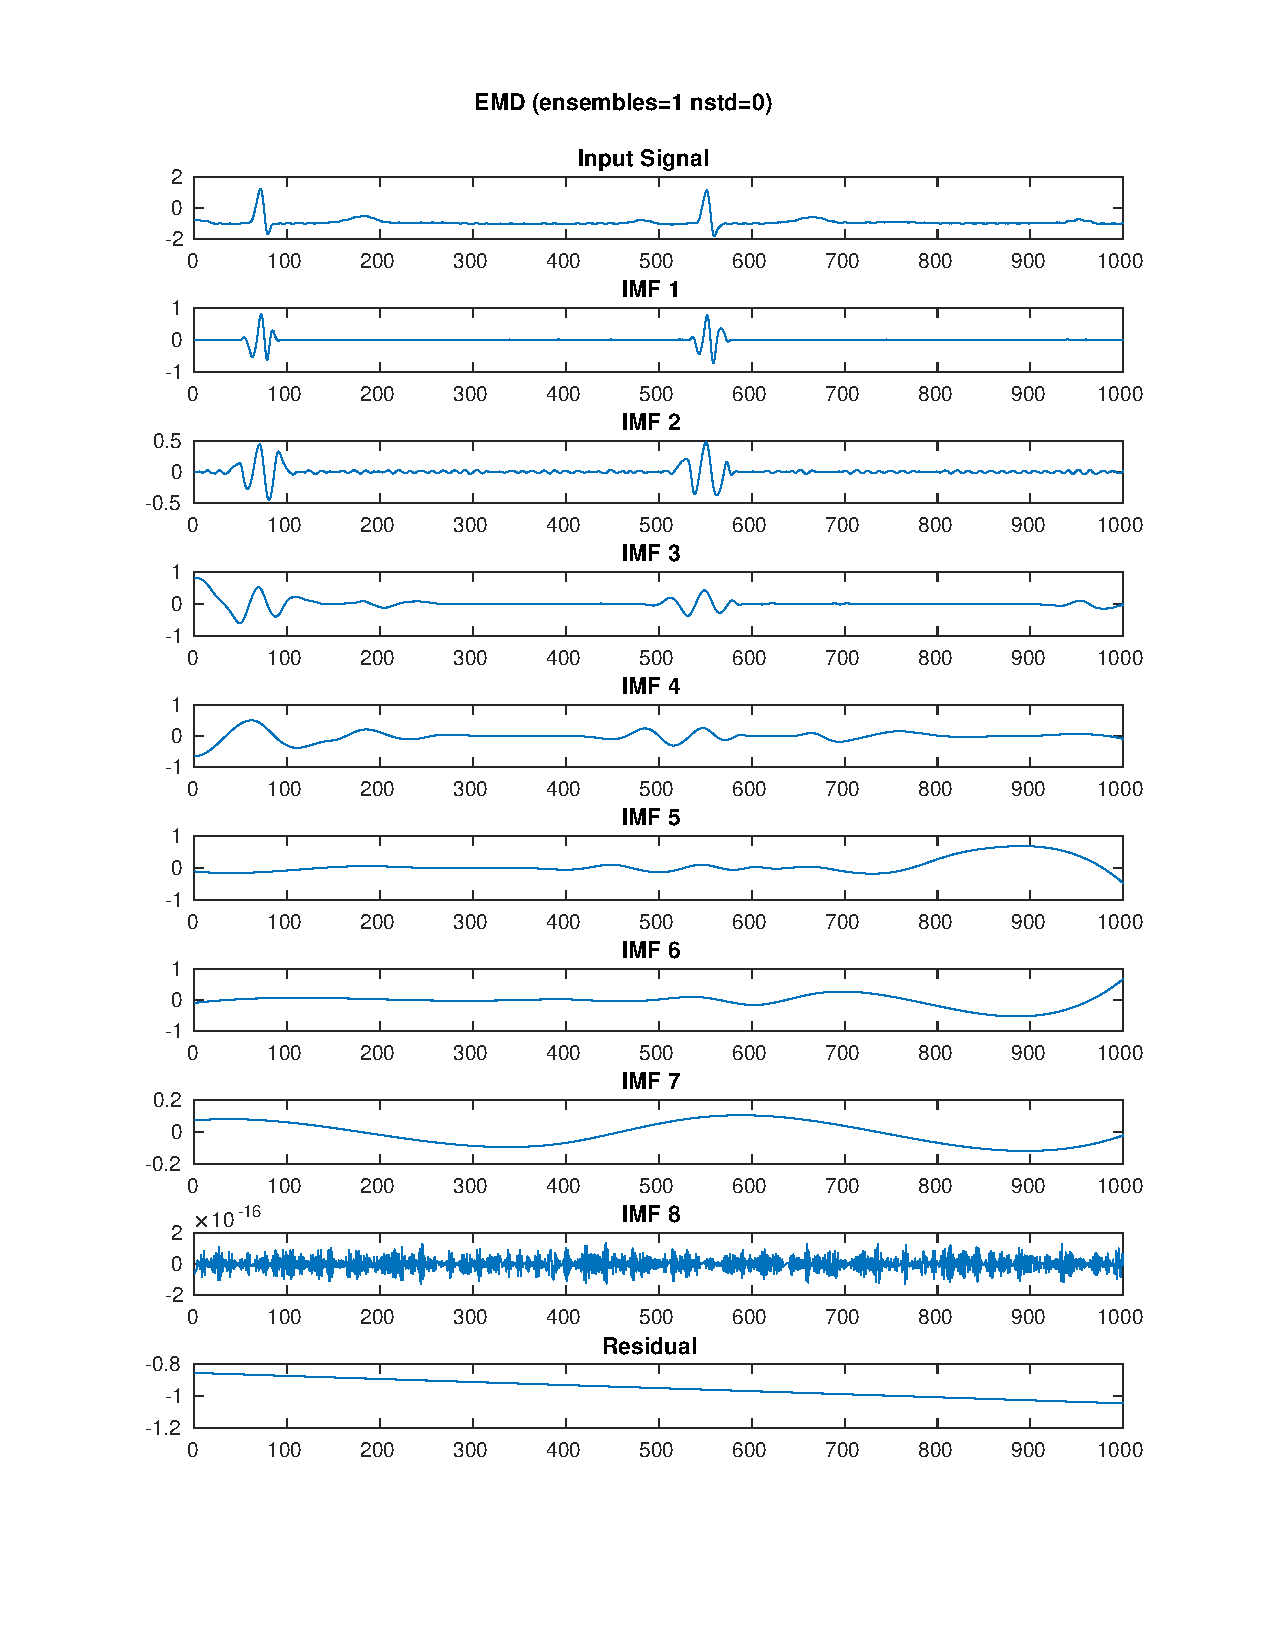
\includegraphics[width=\textwidth]{fig/123l1_emd.pdf}
\end{figure}

\column{0.5\textwidth}
\begin{figure}
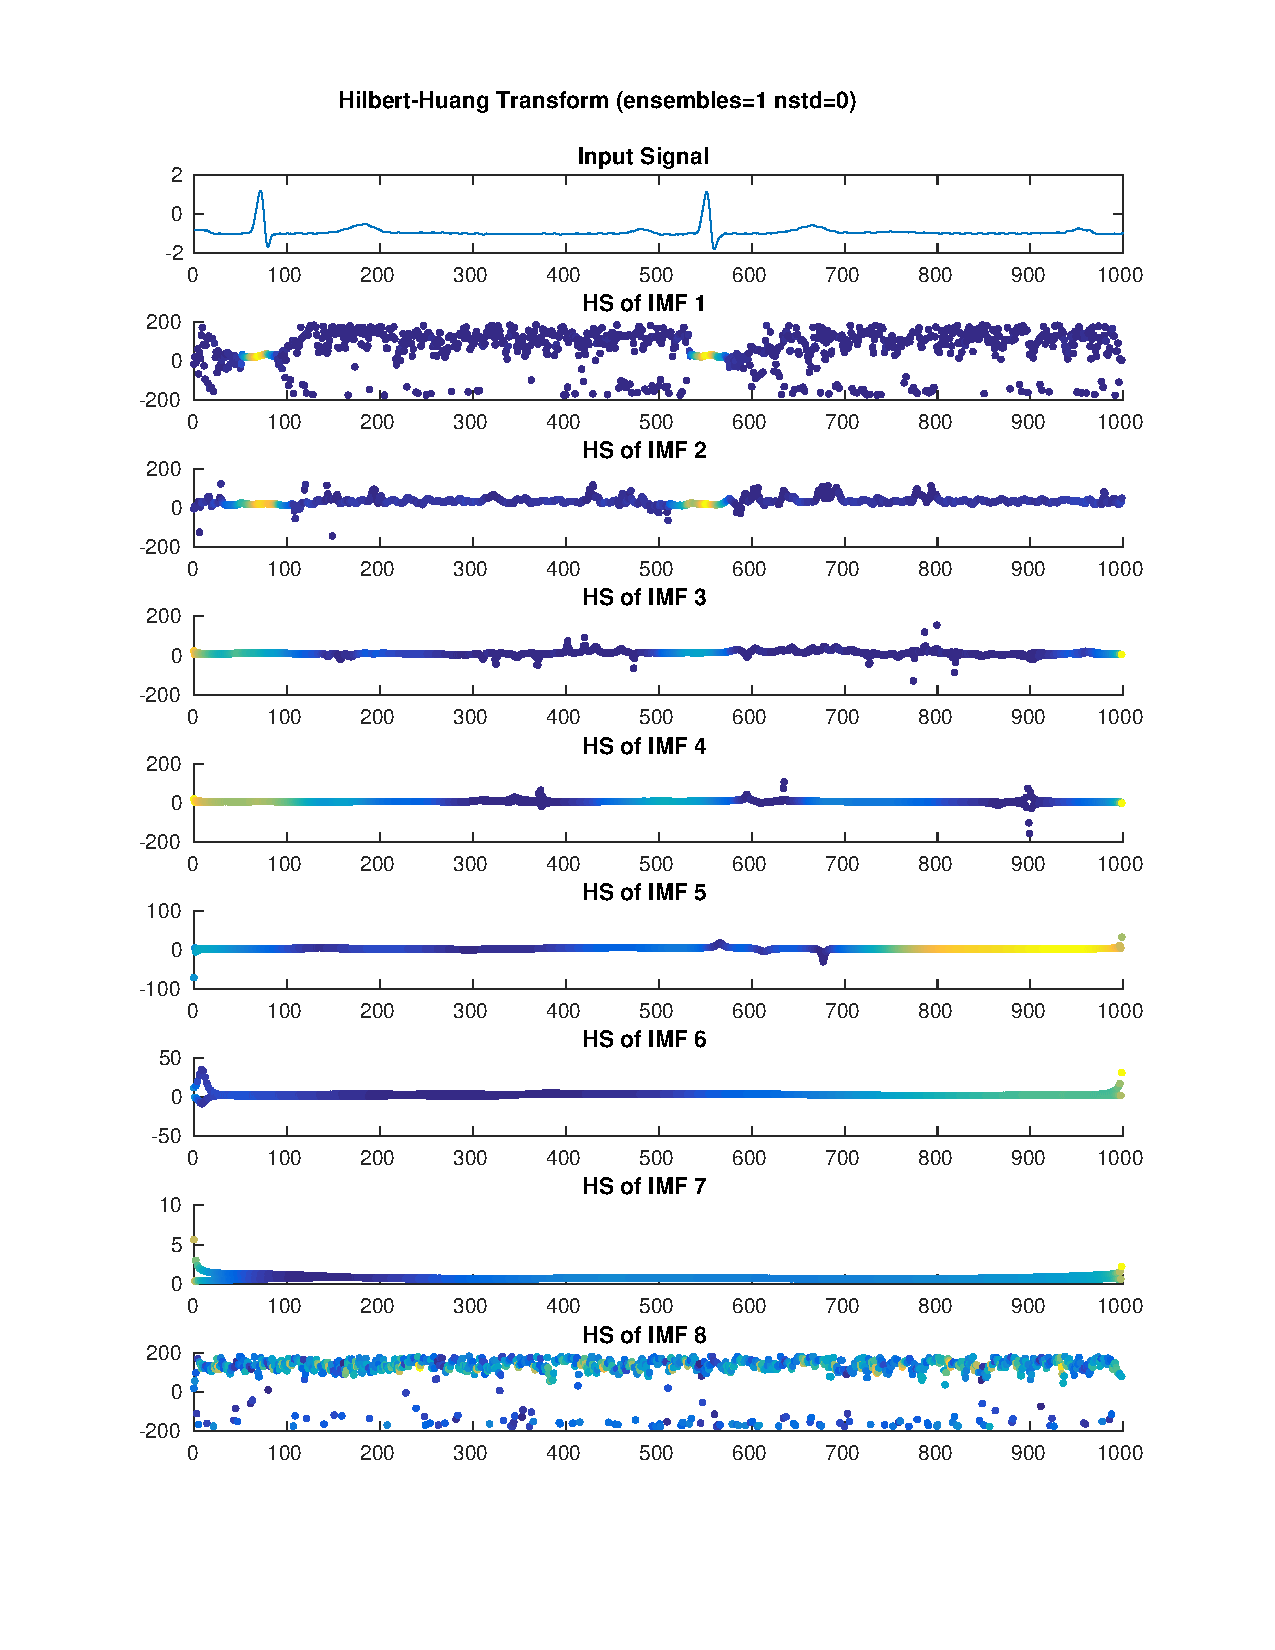
\includegraphics[width=\textwidth]{fig/123l1_hht.pdf}
\end{figure}
\end{columns}
\end{frame}


% --- Ανάλυση 118 ---
\subsection{Σήμα 118}
\label{sig:118}
\begin{frame}
\frametitle{Ανάλυση των σημάτων - 118}

\begin{columns}
\column{0.5\textwidth}
\begin{figure}
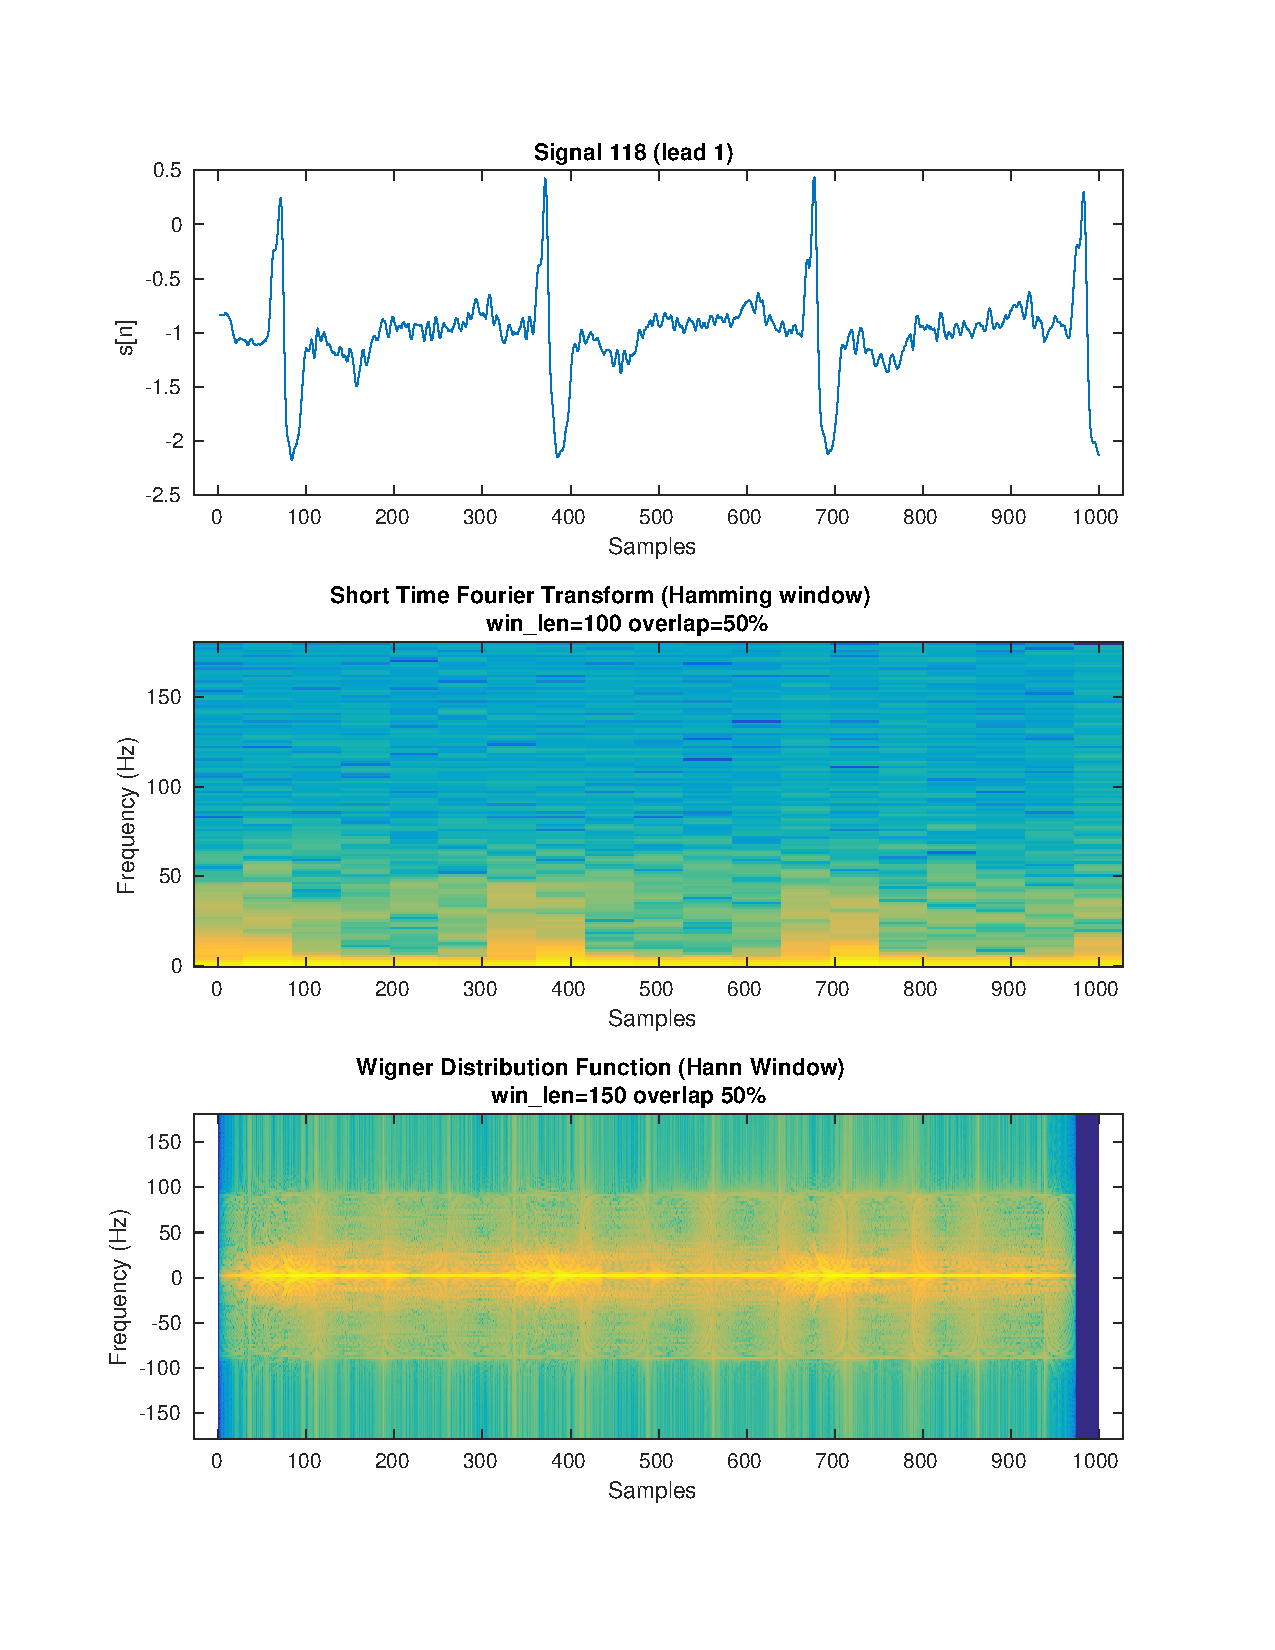
\includegraphics[width=\textwidth]{fig/118l1_stft_wdf.pdf}
\end{figure}

\column{0.5\textwidth}
\begin{figure}
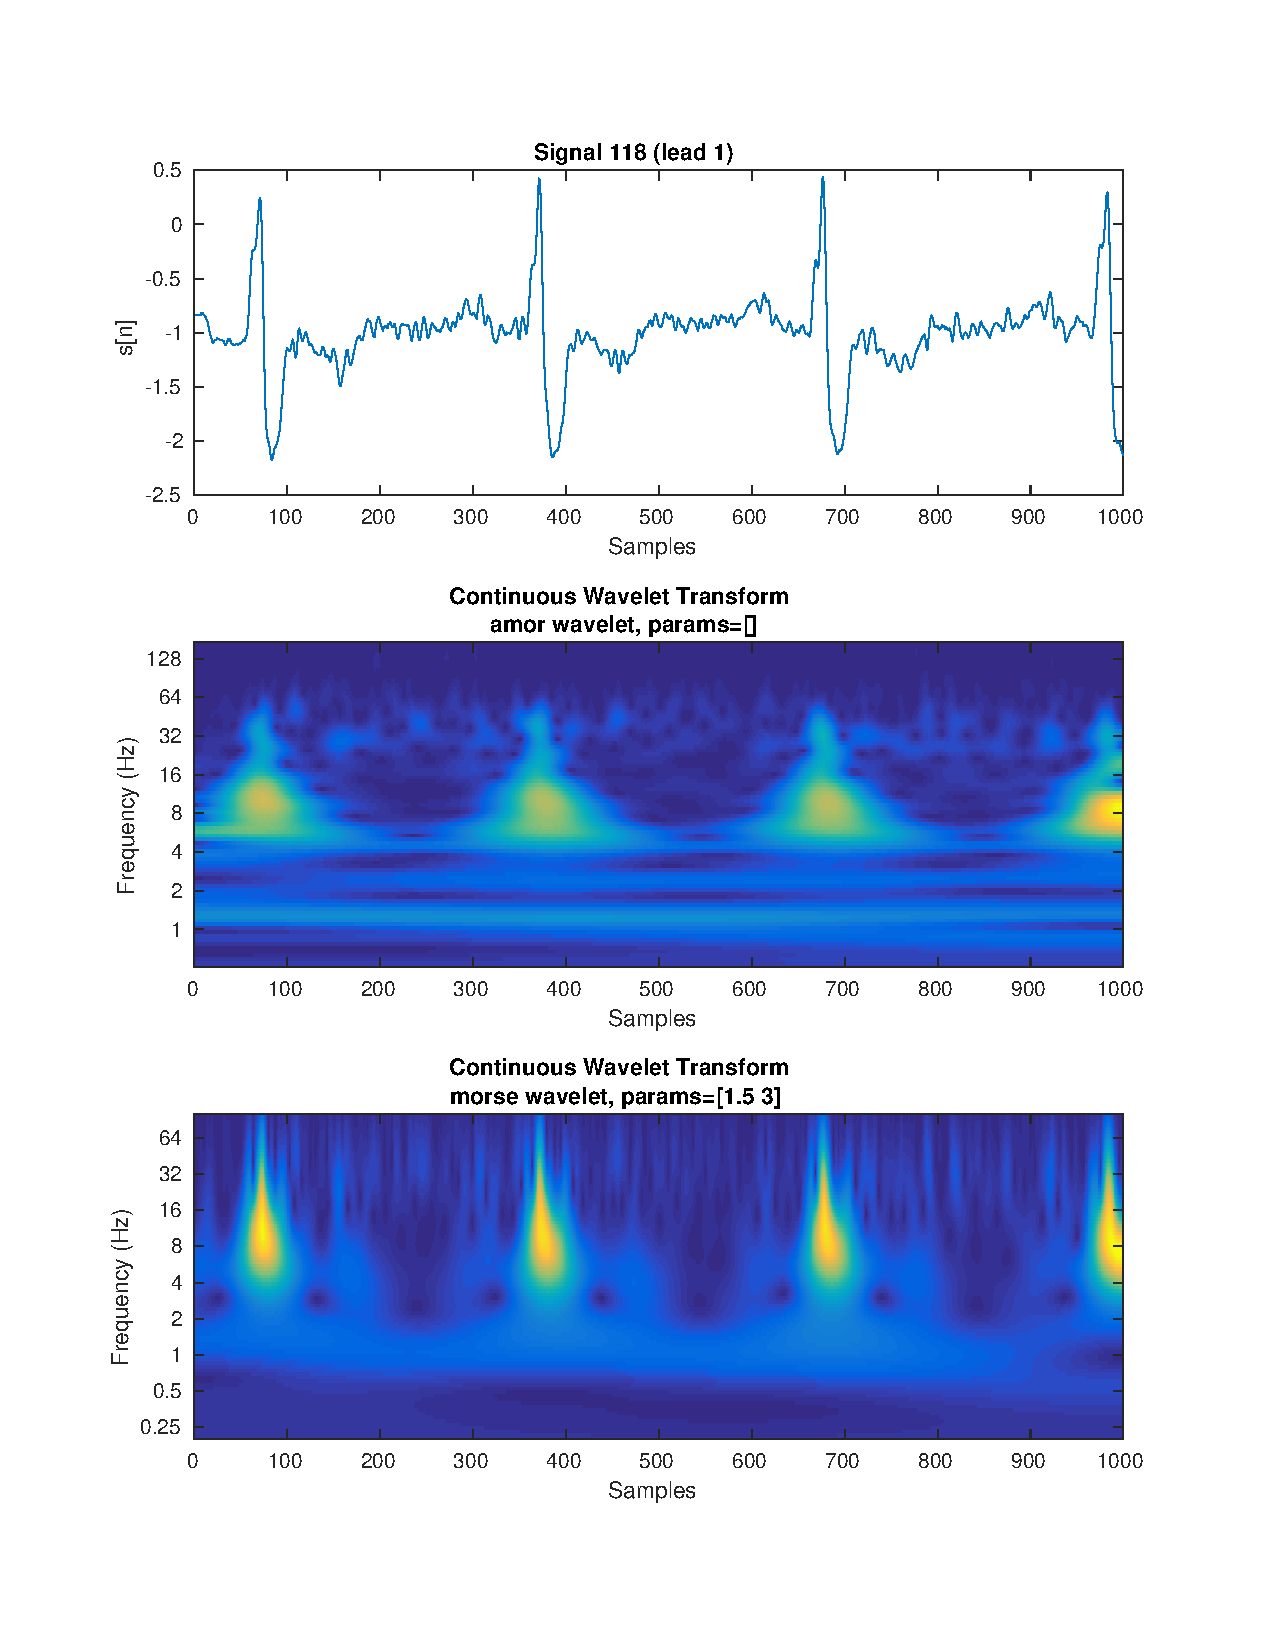
\includegraphics[width=\textwidth]{fig/118l1_cwt.pdf}
\end{figure}
\end{columns}
\end{frame}

\begin{frame}
\frametitle{Ανάλυση των σημάτων - 118}

\begin{columns}
\column{0.5\textwidth}
\begin{figure}
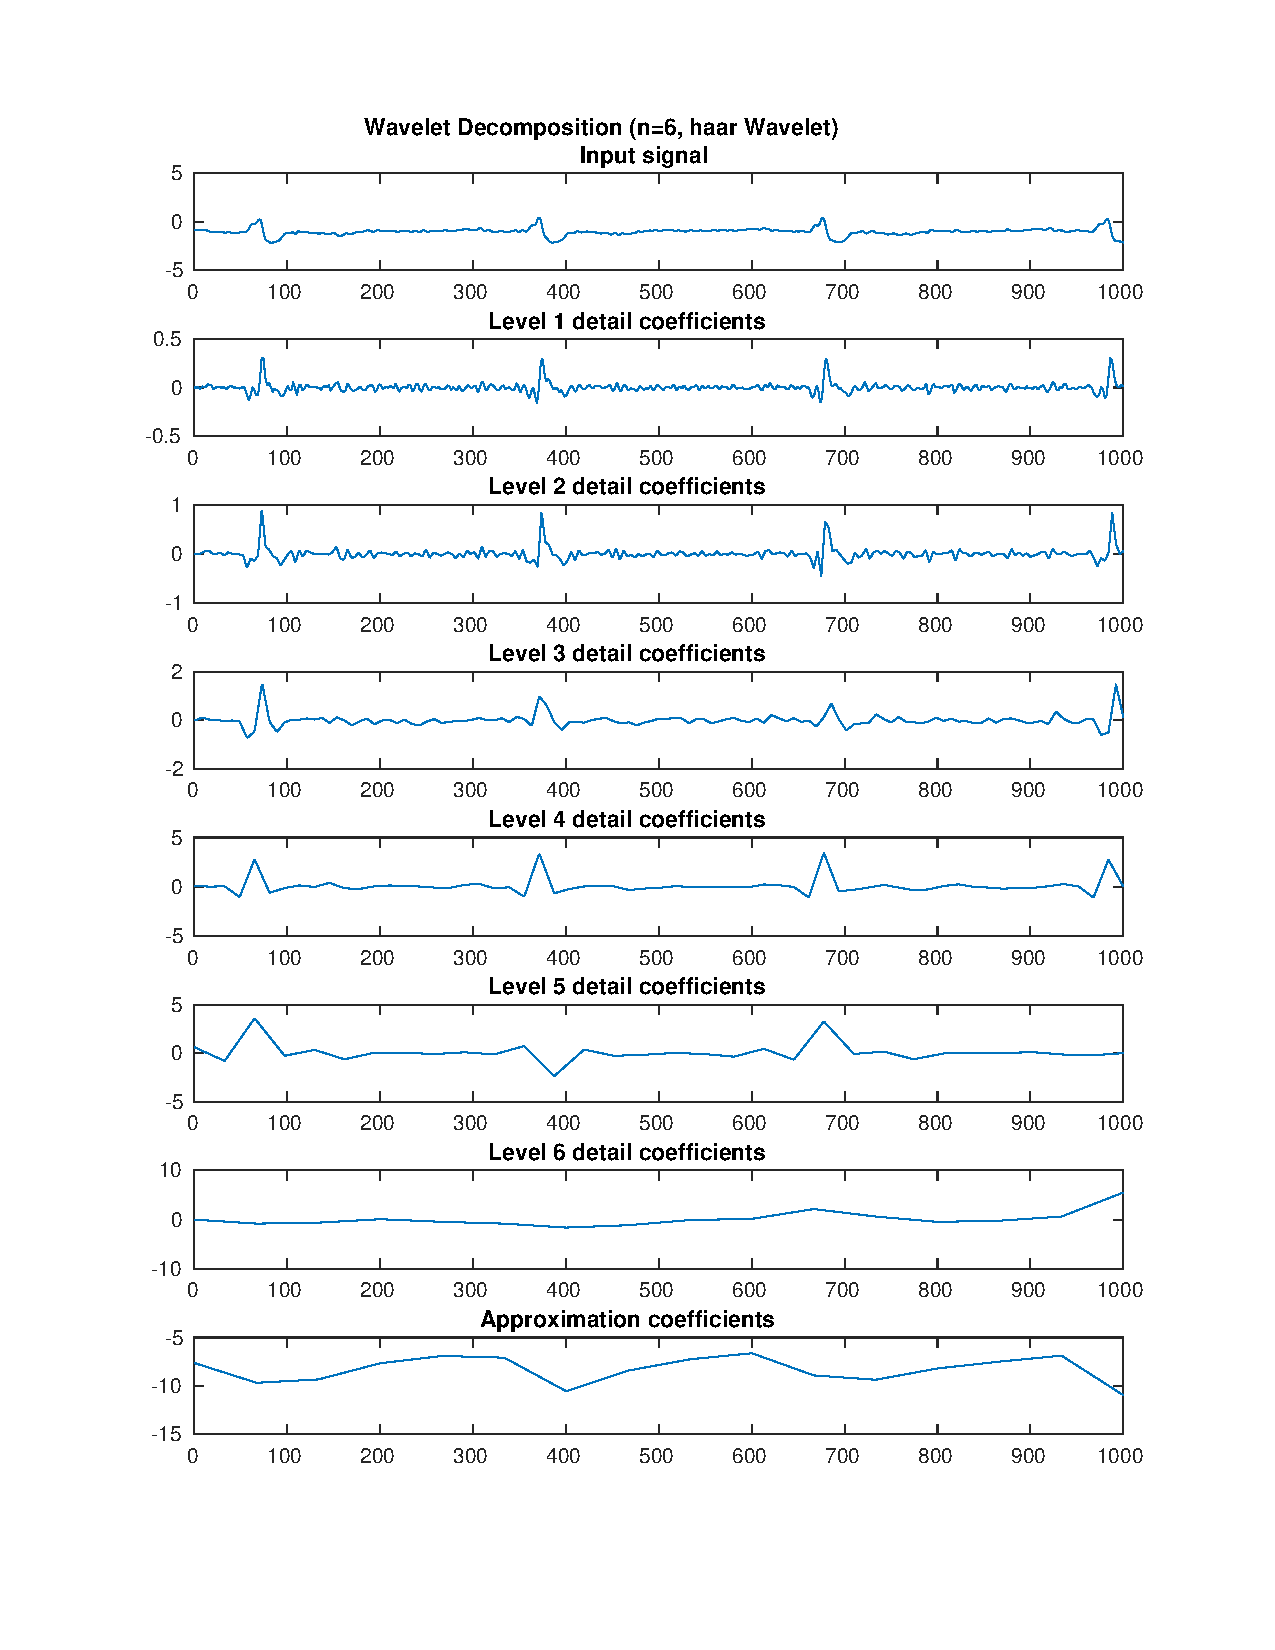
\includegraphics[width=\textwidth]{fig/118l1_dwt1.pdf}
\end{figure}

\column{0.5\textwidth}
\begin{figure}
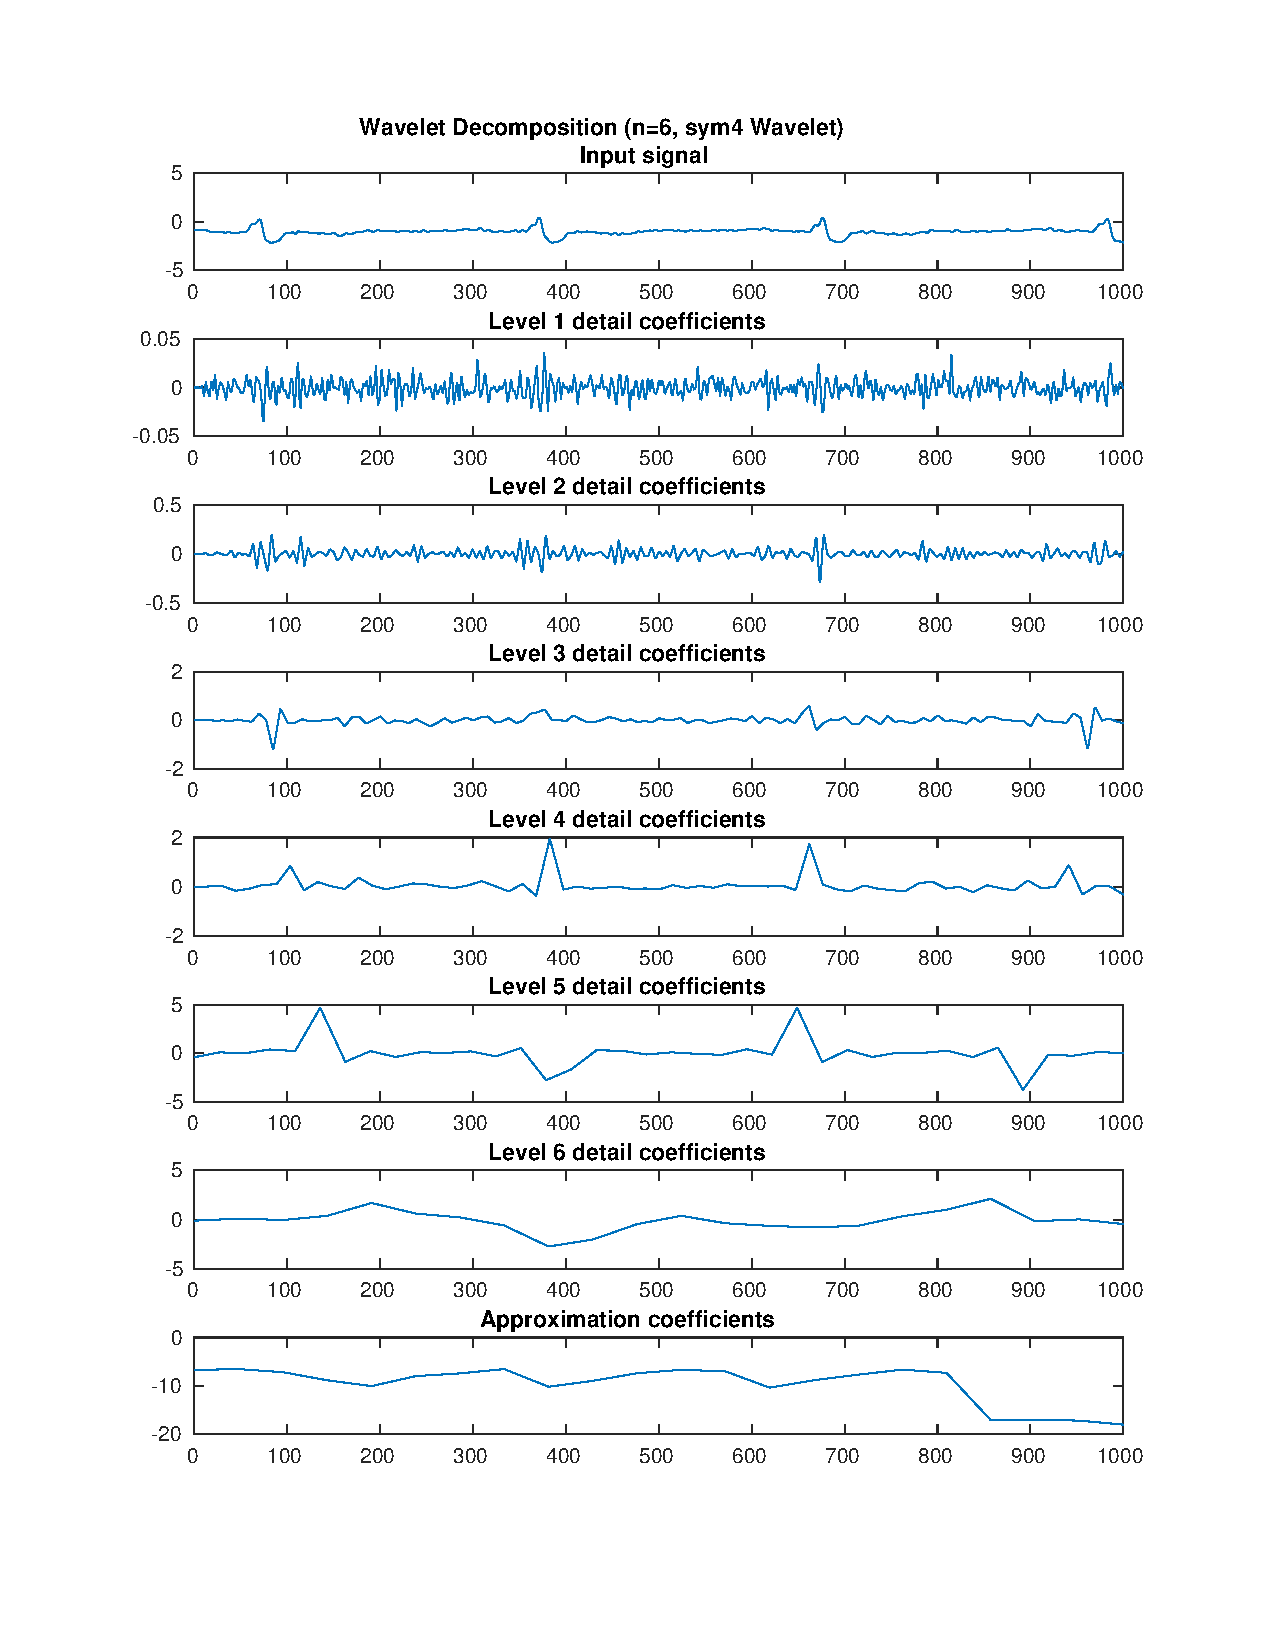
\includegraphics[width=\textwidth]{fig/118l1_dwt2.pdf}
\end{figure}
\end{columns}
\end{frame}

\begin{frame}
\frametitle{Ανάλυση των σημάτων - 118}

\begin{columns}
\column{0.5\textwidth}
\begin{figure}
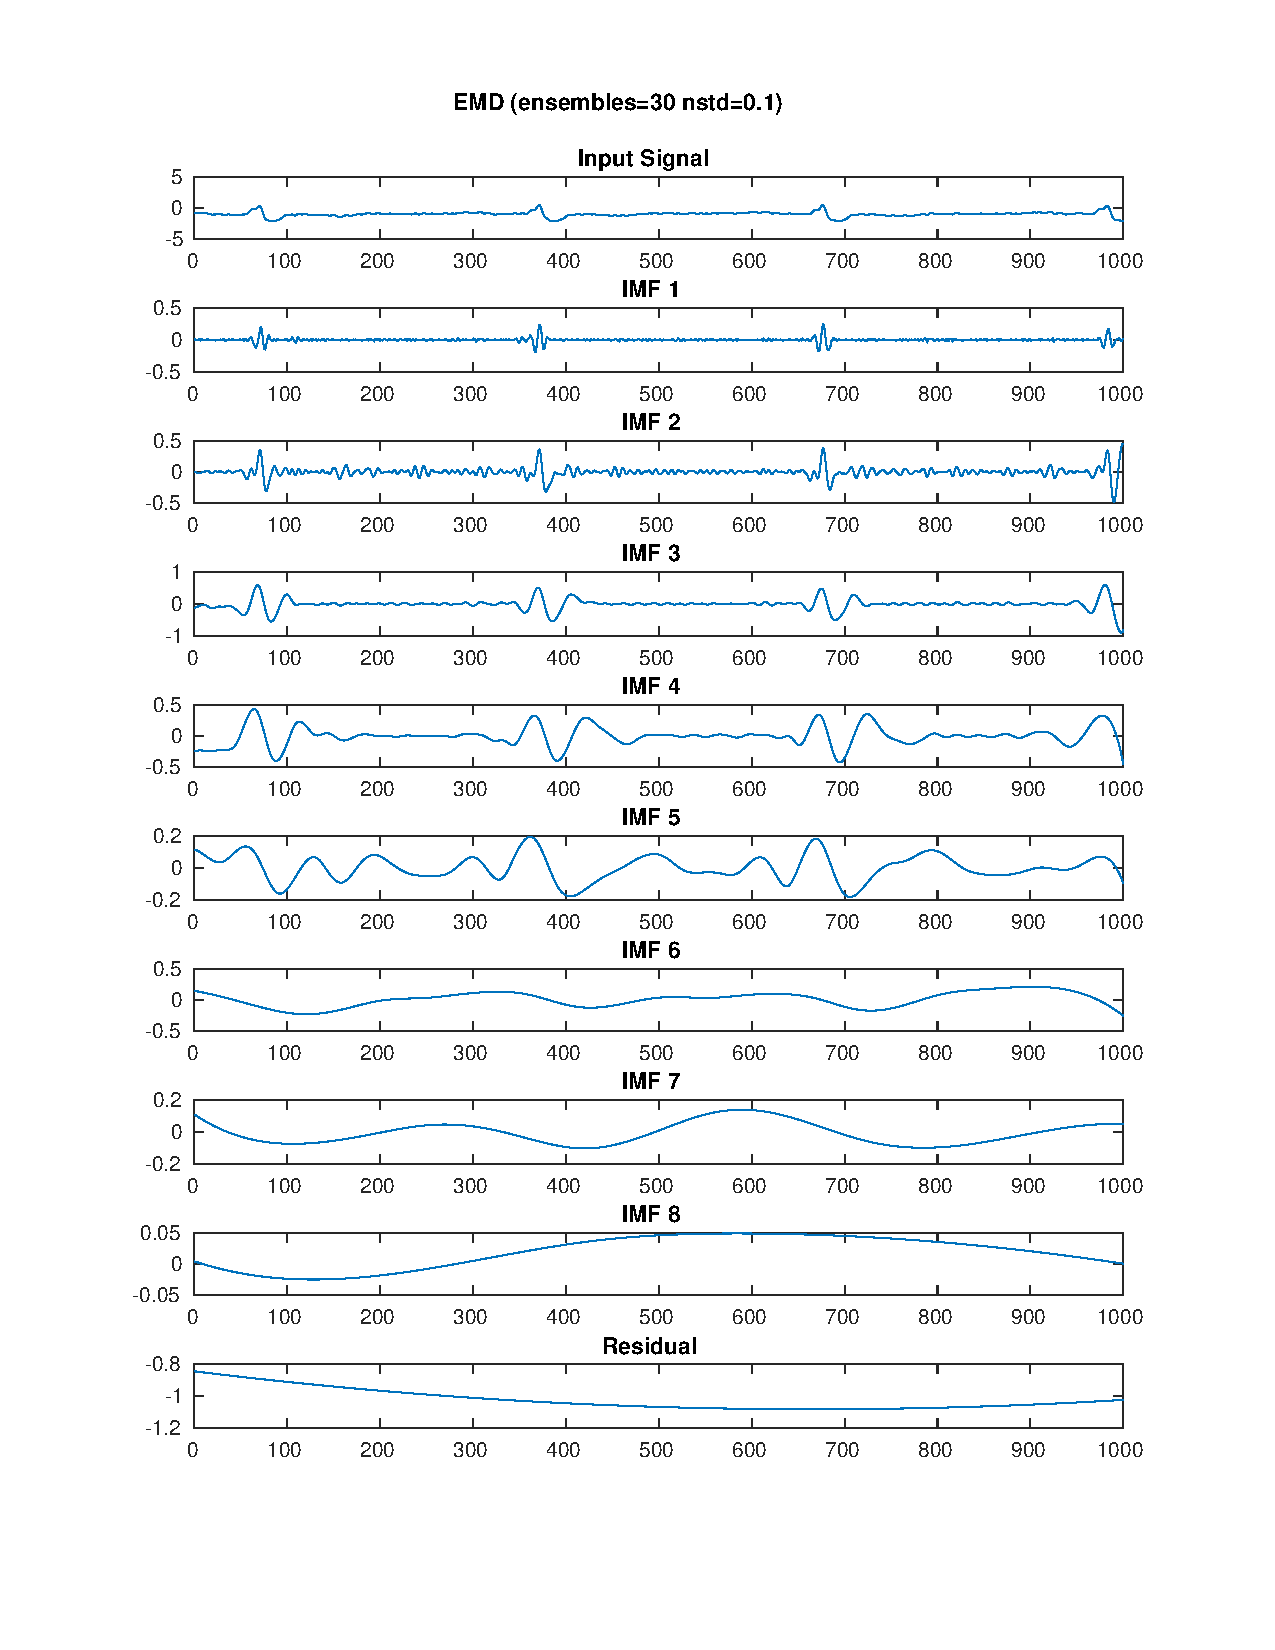
\includegraphics[width=\textwidth]{fig/118l1_emd_ensemble.pdf}
\end{figure}

\column{0.5\textwidth}
\begin{figure}
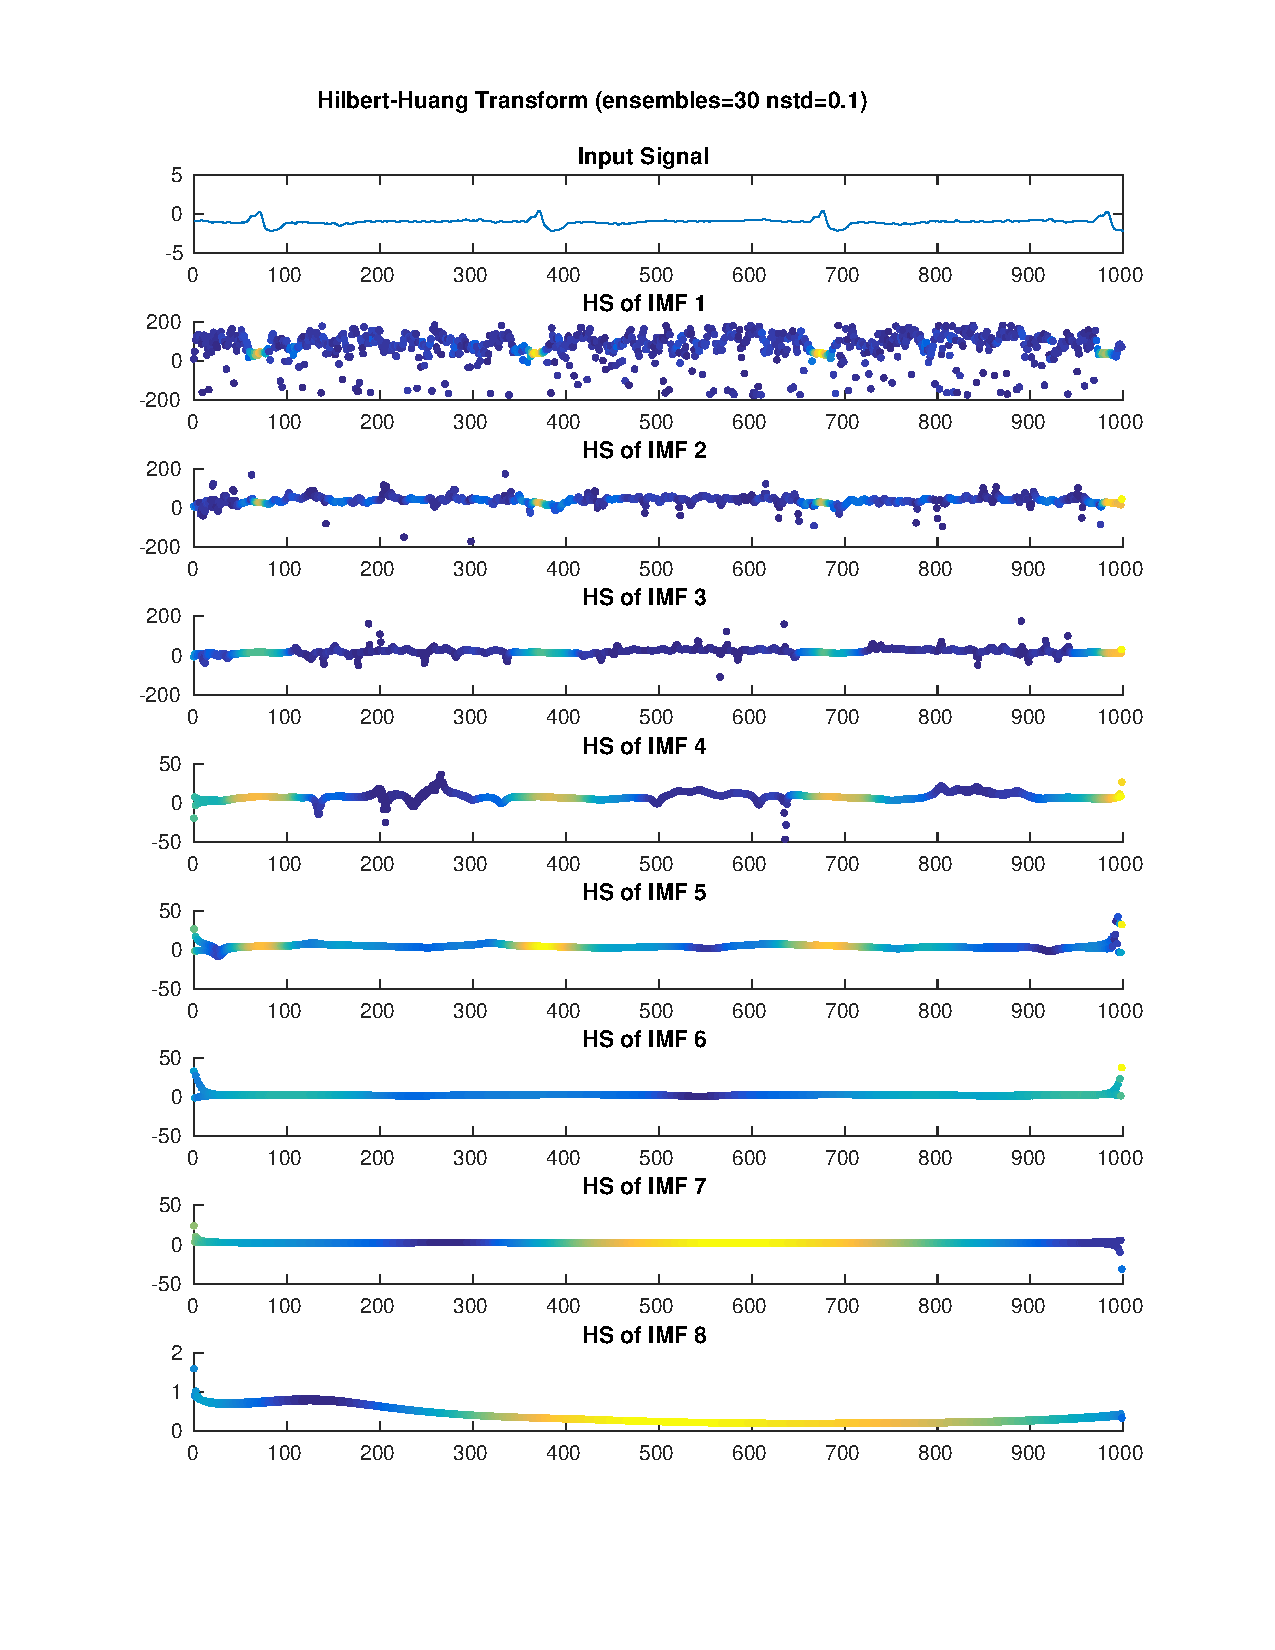
\includegraphics[width=\textwidth]{fig/118l1_hht_ensemble.pdf}
\end{figure}
\end{columns}
\end{frame}


% --- Ανάλυση 217 ---
\subsection{Σήμα 217}
\label{sig:217}
\begin{frame}
\frametitle{Ανάλυση των σημάτων - 217}

\begin{columns}
\column{0.5\textwidth}
\begin{figure}
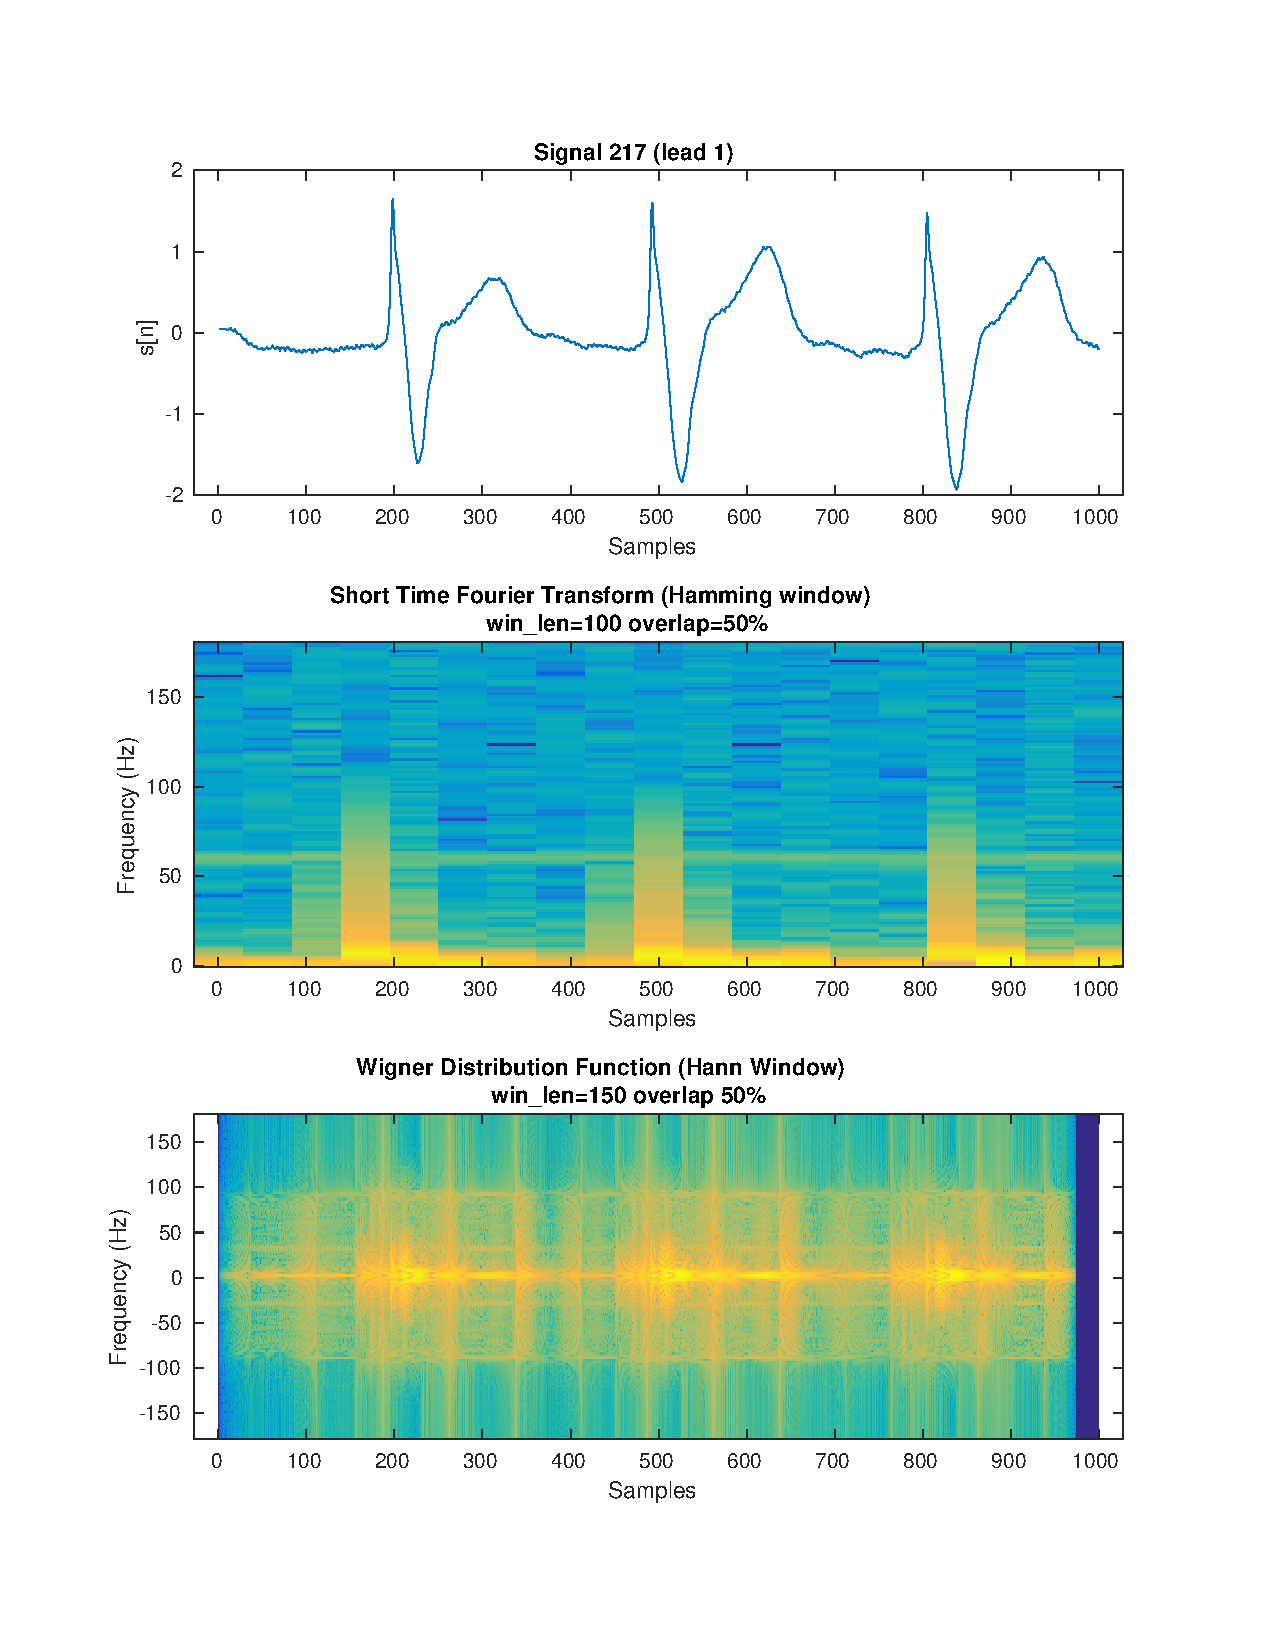
\includegraphics[width=\textwidth]{fig/217l1_stft_wdf.pdf}
\end{figure}

\column{0.5\textwidth}
\begin{figure}
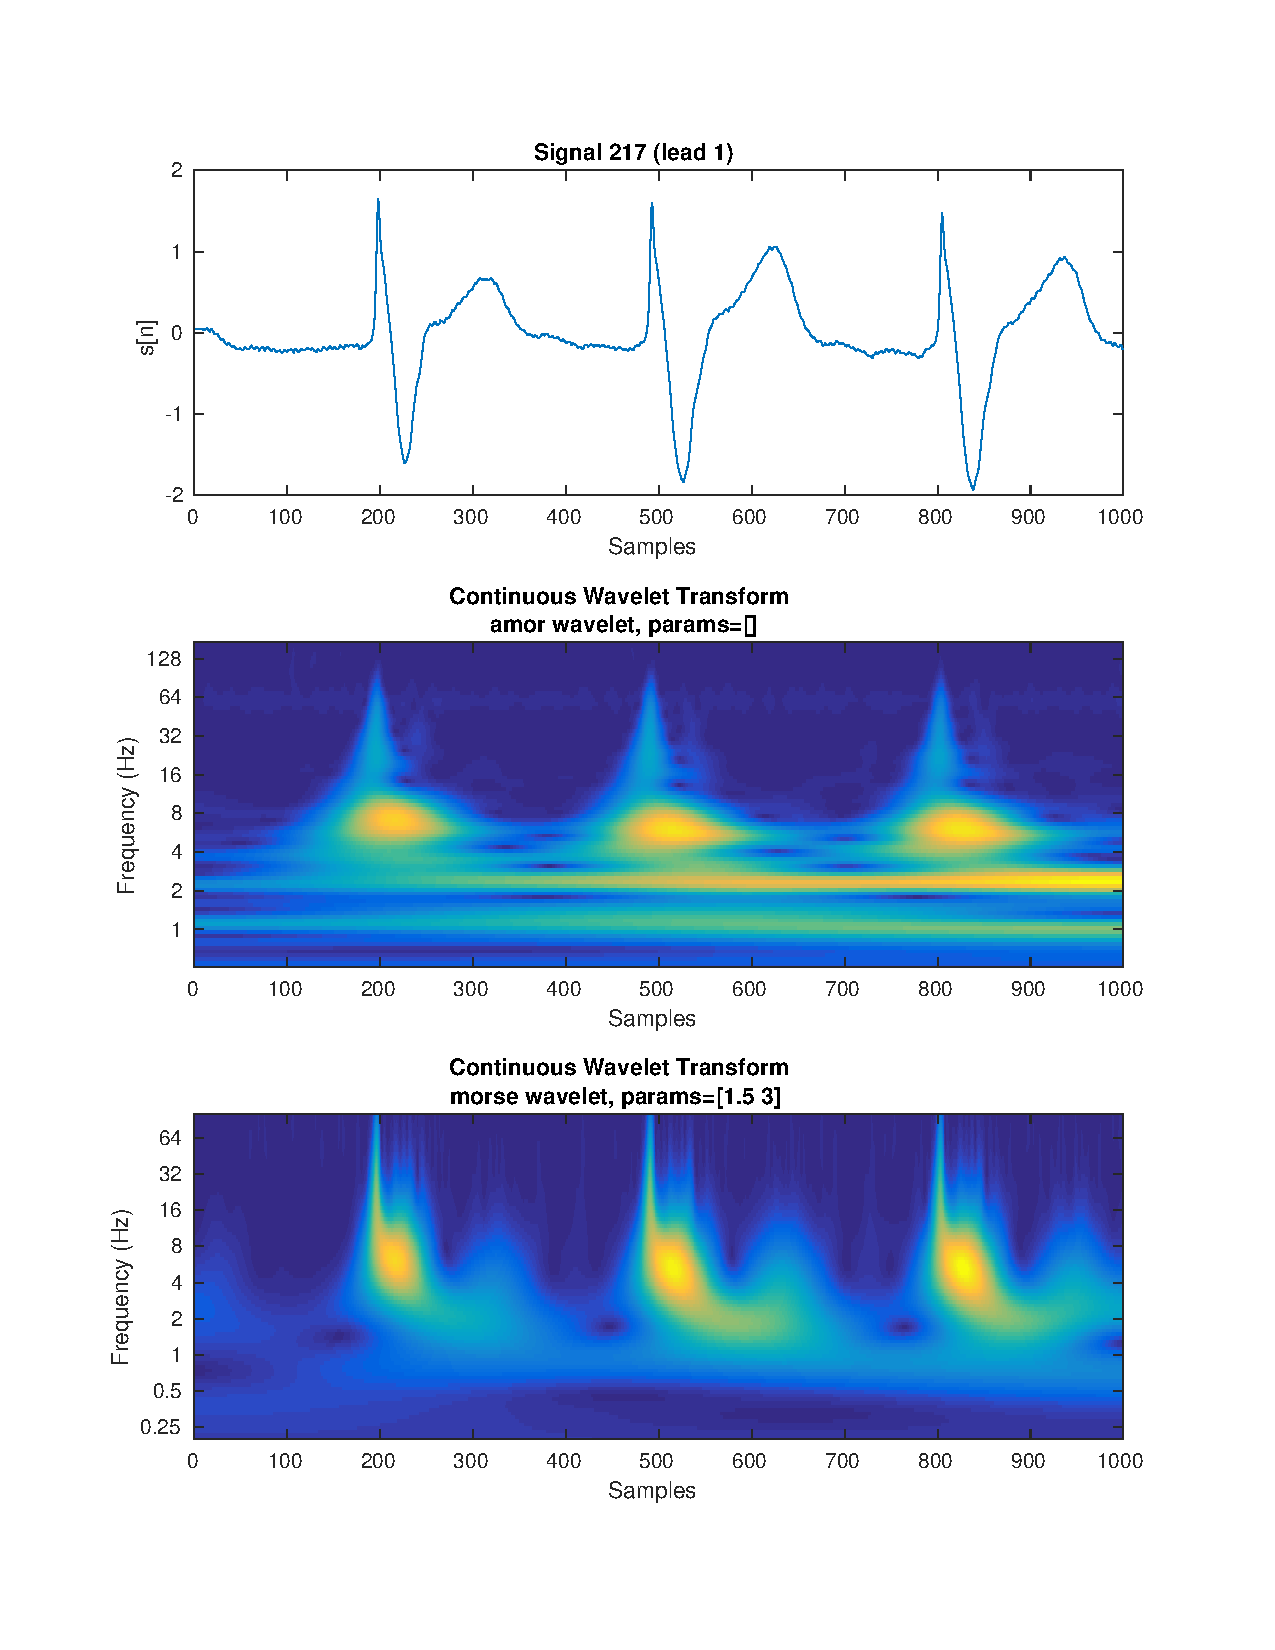
\includegraphics[width=\textwidth]{fig/217l1_cwt.pdf}
\end{figure}
\end{columns}
\end{frame}

\begin{frame}
\frametitle{Ανάλυση των σημάτων - 217}

\begin{columns}
\column{0.5\textwidth}
\begin{figure}
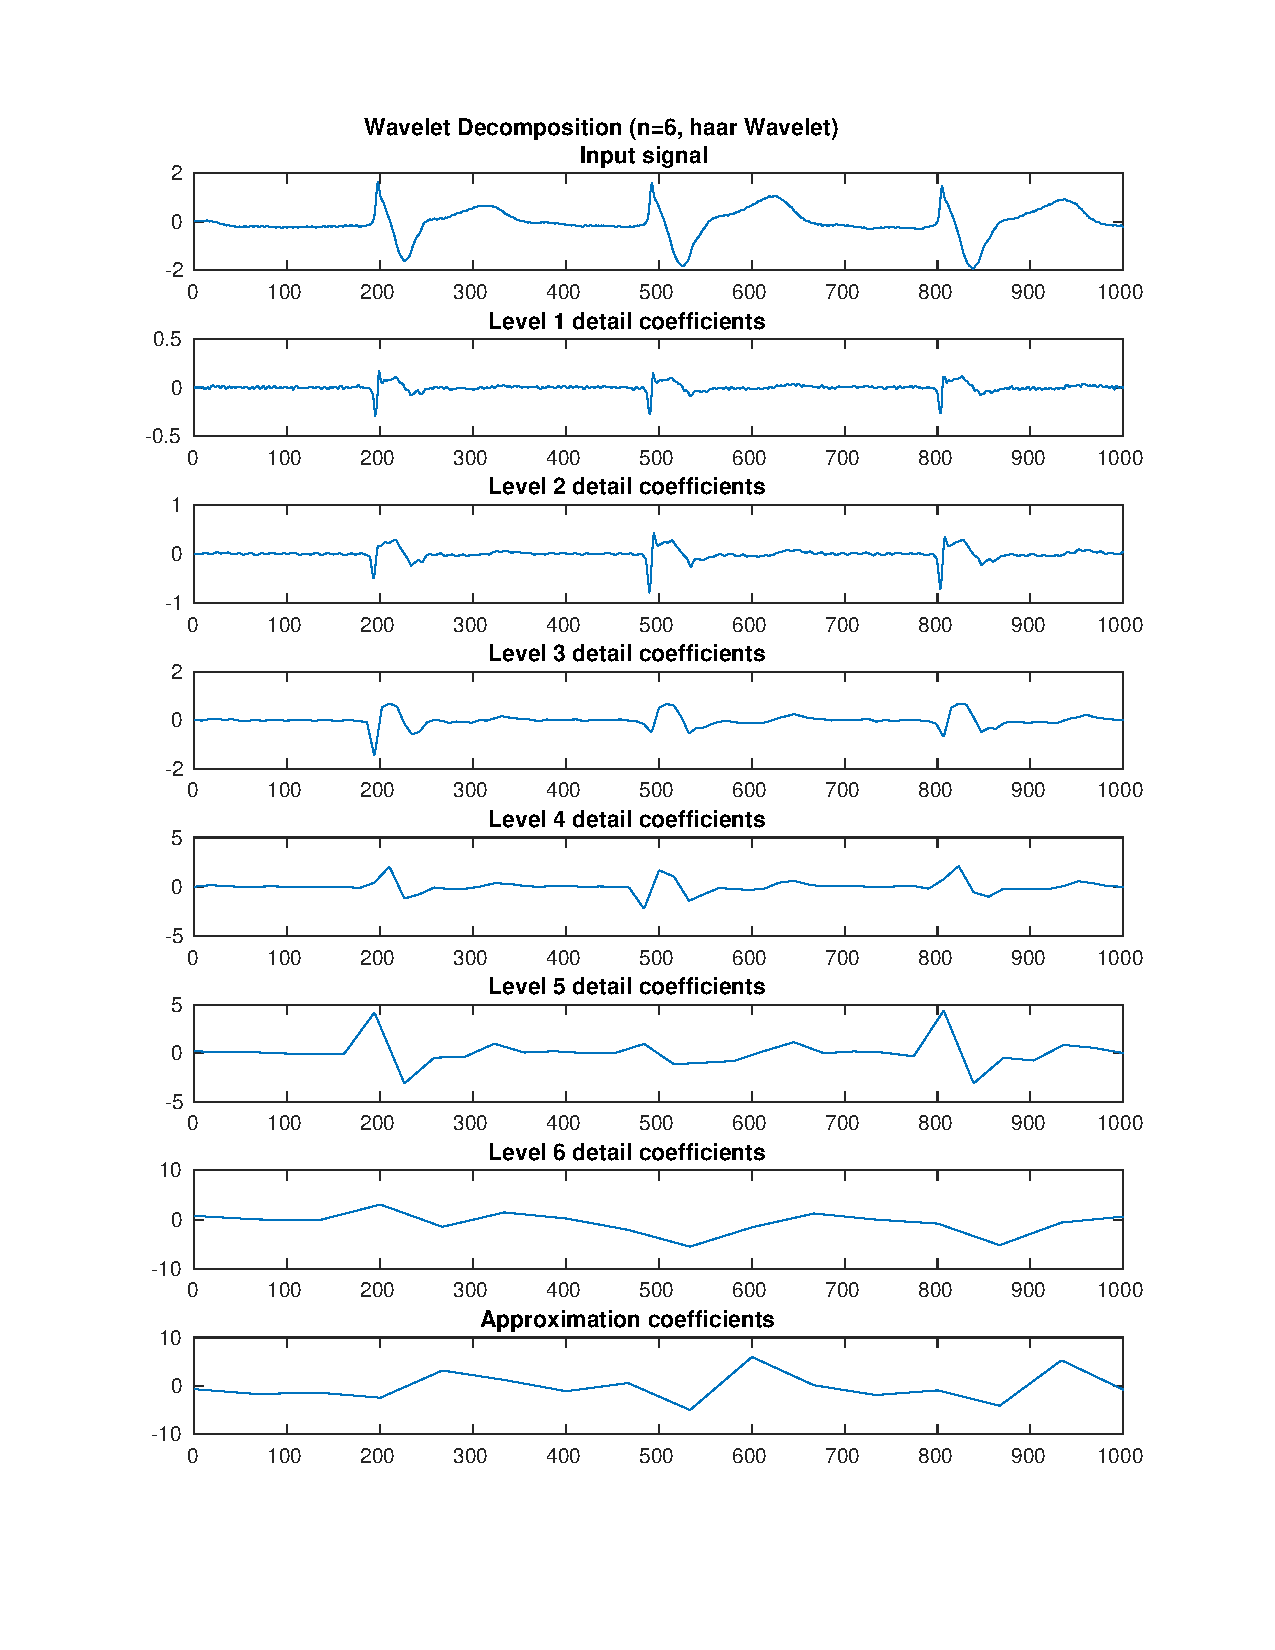
\includegraphics[width=\textwidth]{fig/217l1_dwt1.pdf}
\end{figure}

\column{0.5\textwidth}
\begin{figure}
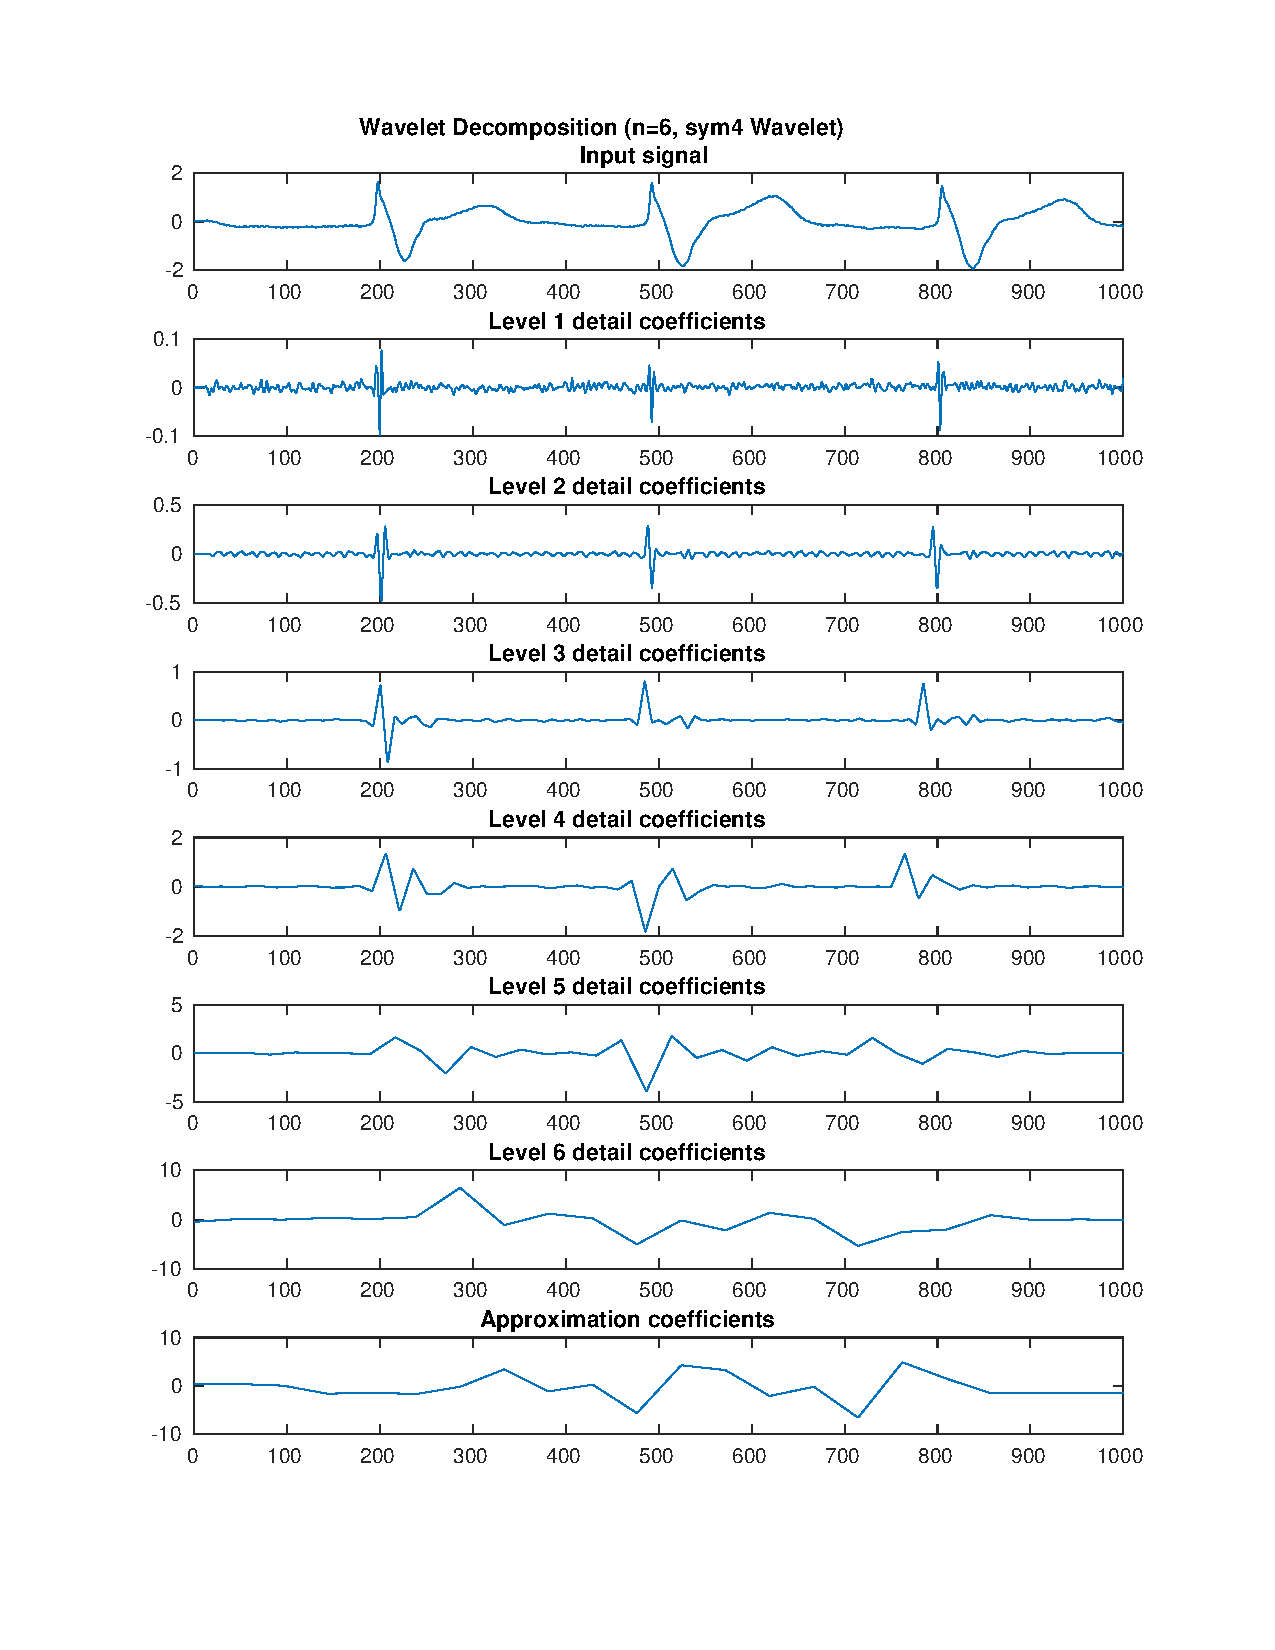
\includegraphics[width=\textwidth]{fig/217l1_dwt2.pdf}
\end{figure}
\end{columns}
\end{frame}

\begin{frame}
\frametitle{Ανάλυση των σημάτων - 217}

\begin{columns}
\column{0.5\textwidth}
\begin{figure}
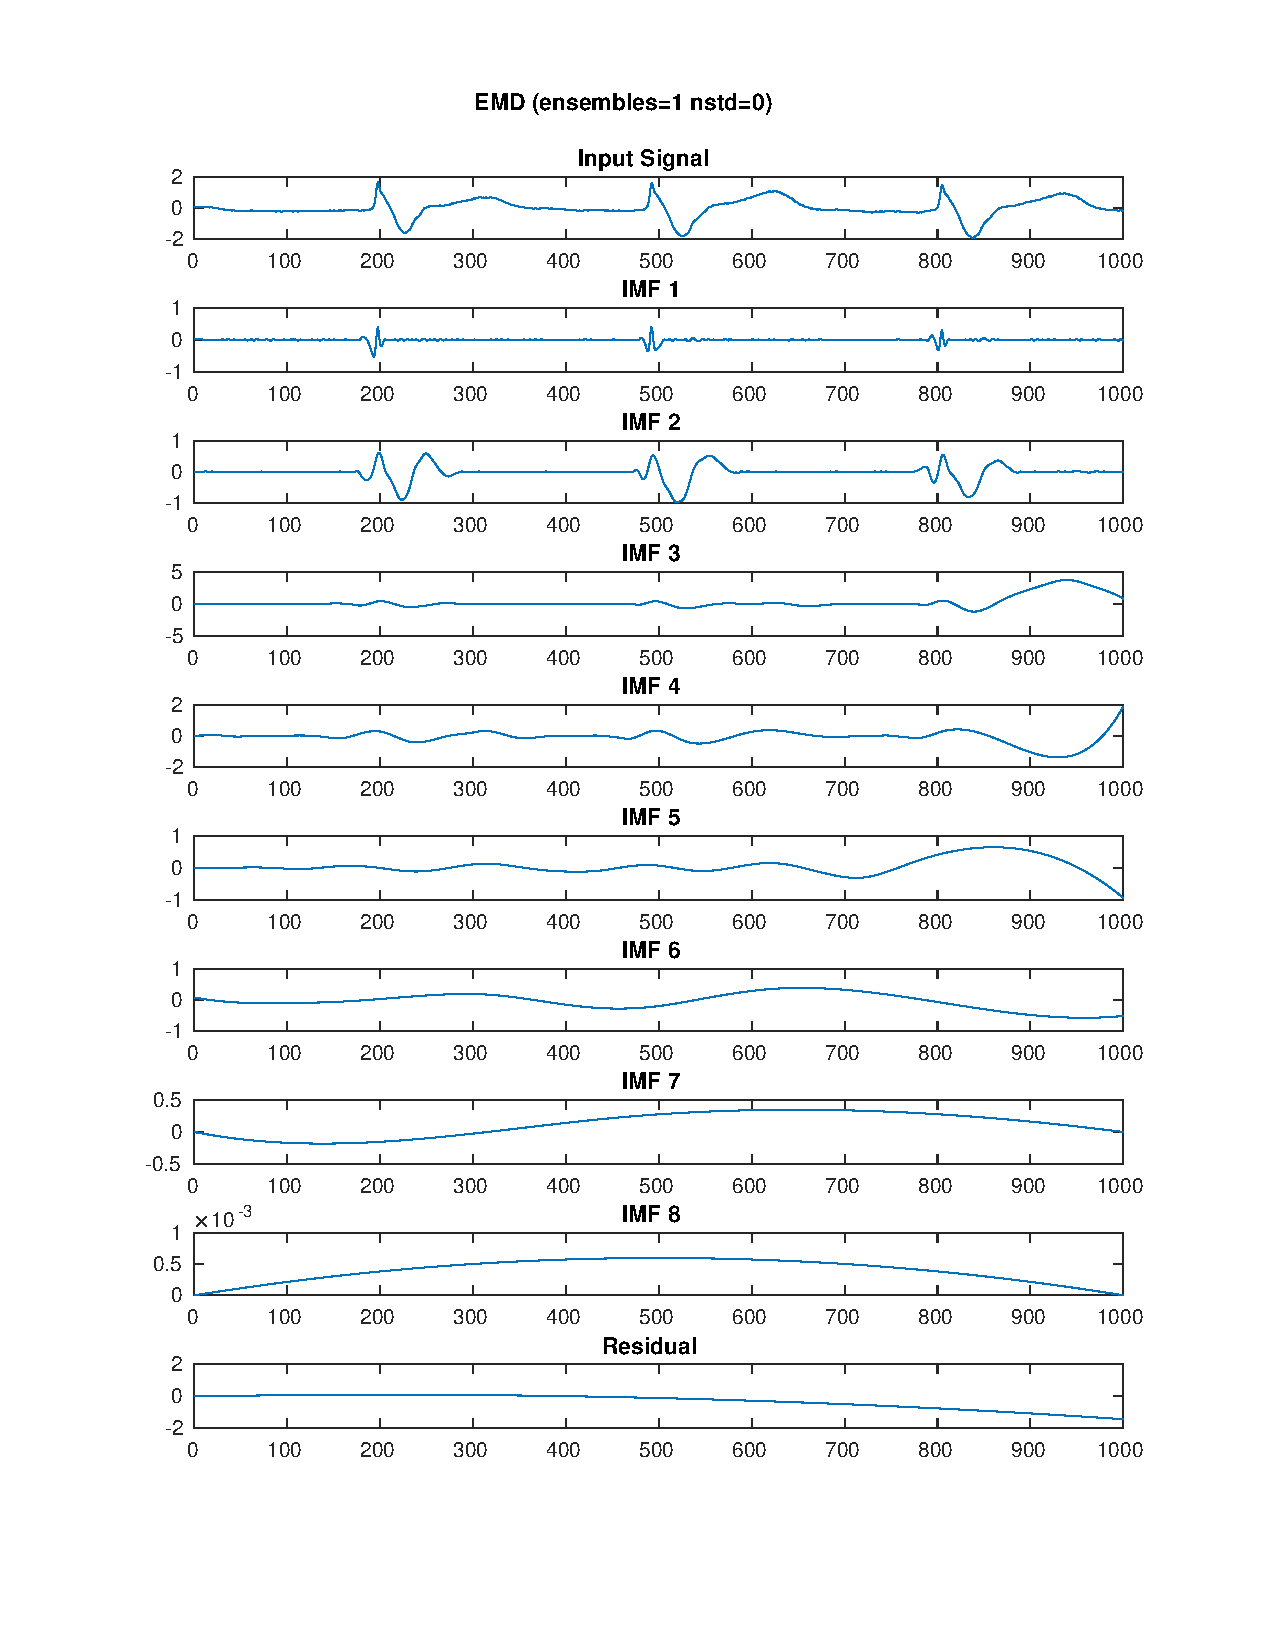
\includegraphics[width=\textwidth]{fig/217l1_emd.pdf}
\end{figure}

\column{0.5\textwidth}
\begin{figure}
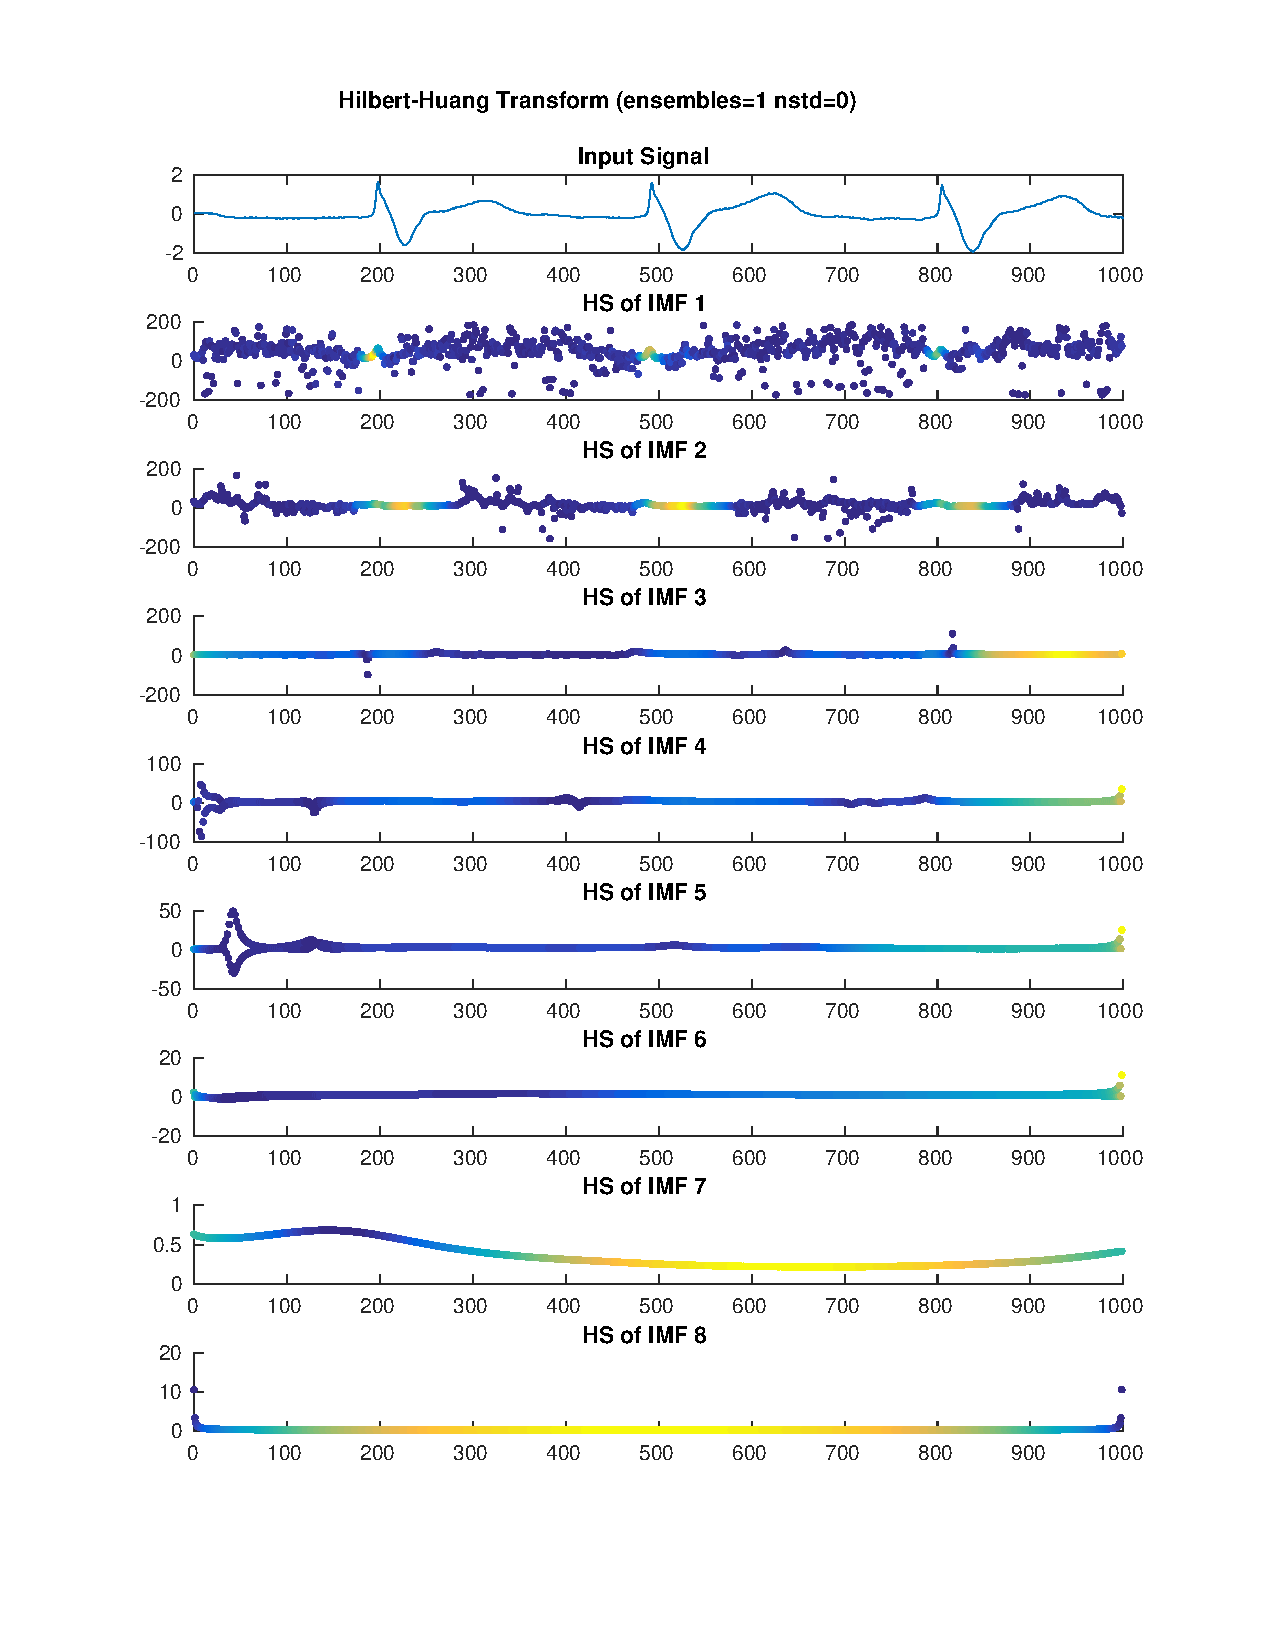
\includegraphics[width=\textwidth]{fig/217l1_hht.pdf}
\end{figure}
\end{columns}
\end{frame}


% --- Ανάλυση 221 ---
\subsection{Σήμα 221}
\label{sig:221}
\begin{frame}
\frametitle{Ανάλυση των σημάτων - 221}

\begin{columns}
\column{0.5\textwidth}
\begin{figure}
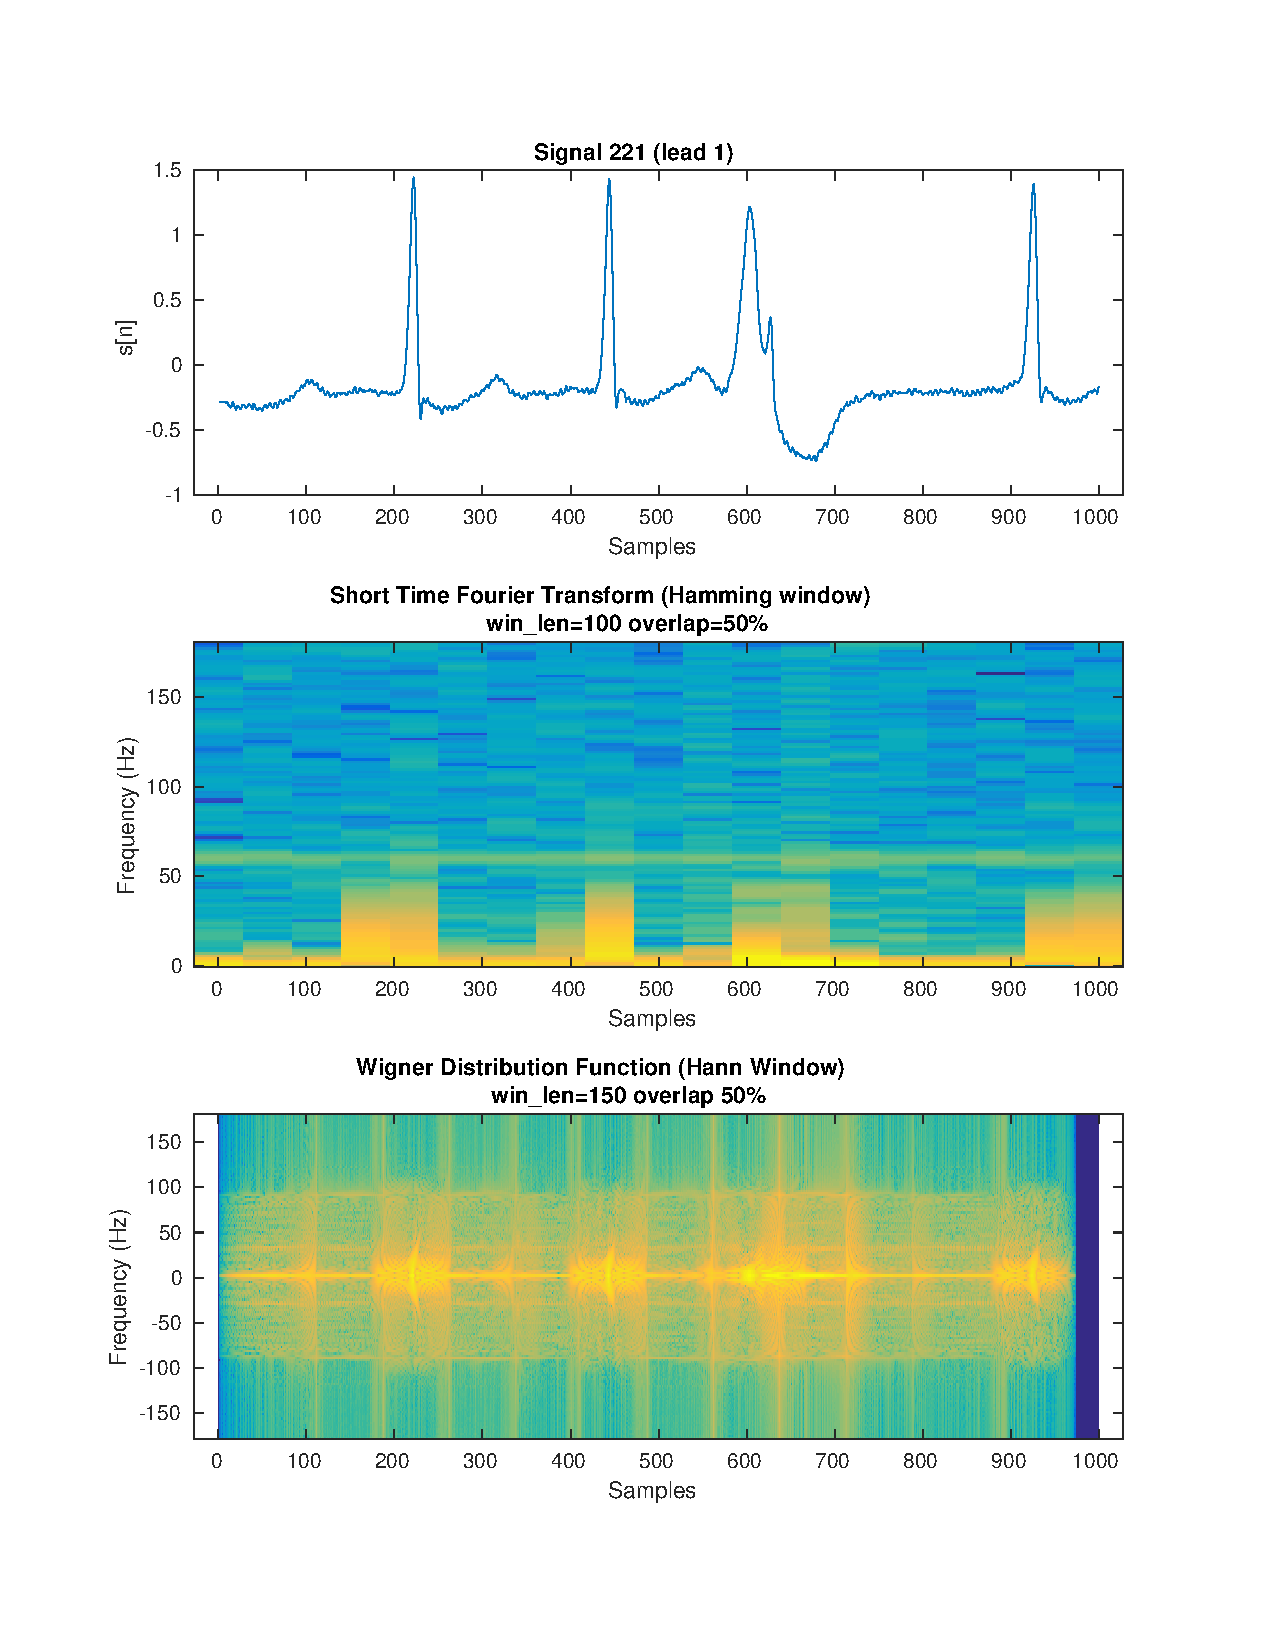
\includegraphics[width=\textwidth]{fig/221l1_stft_wdf.pdf}
\end{figure}

\column{0.5\textwidth}
\begin{figure}
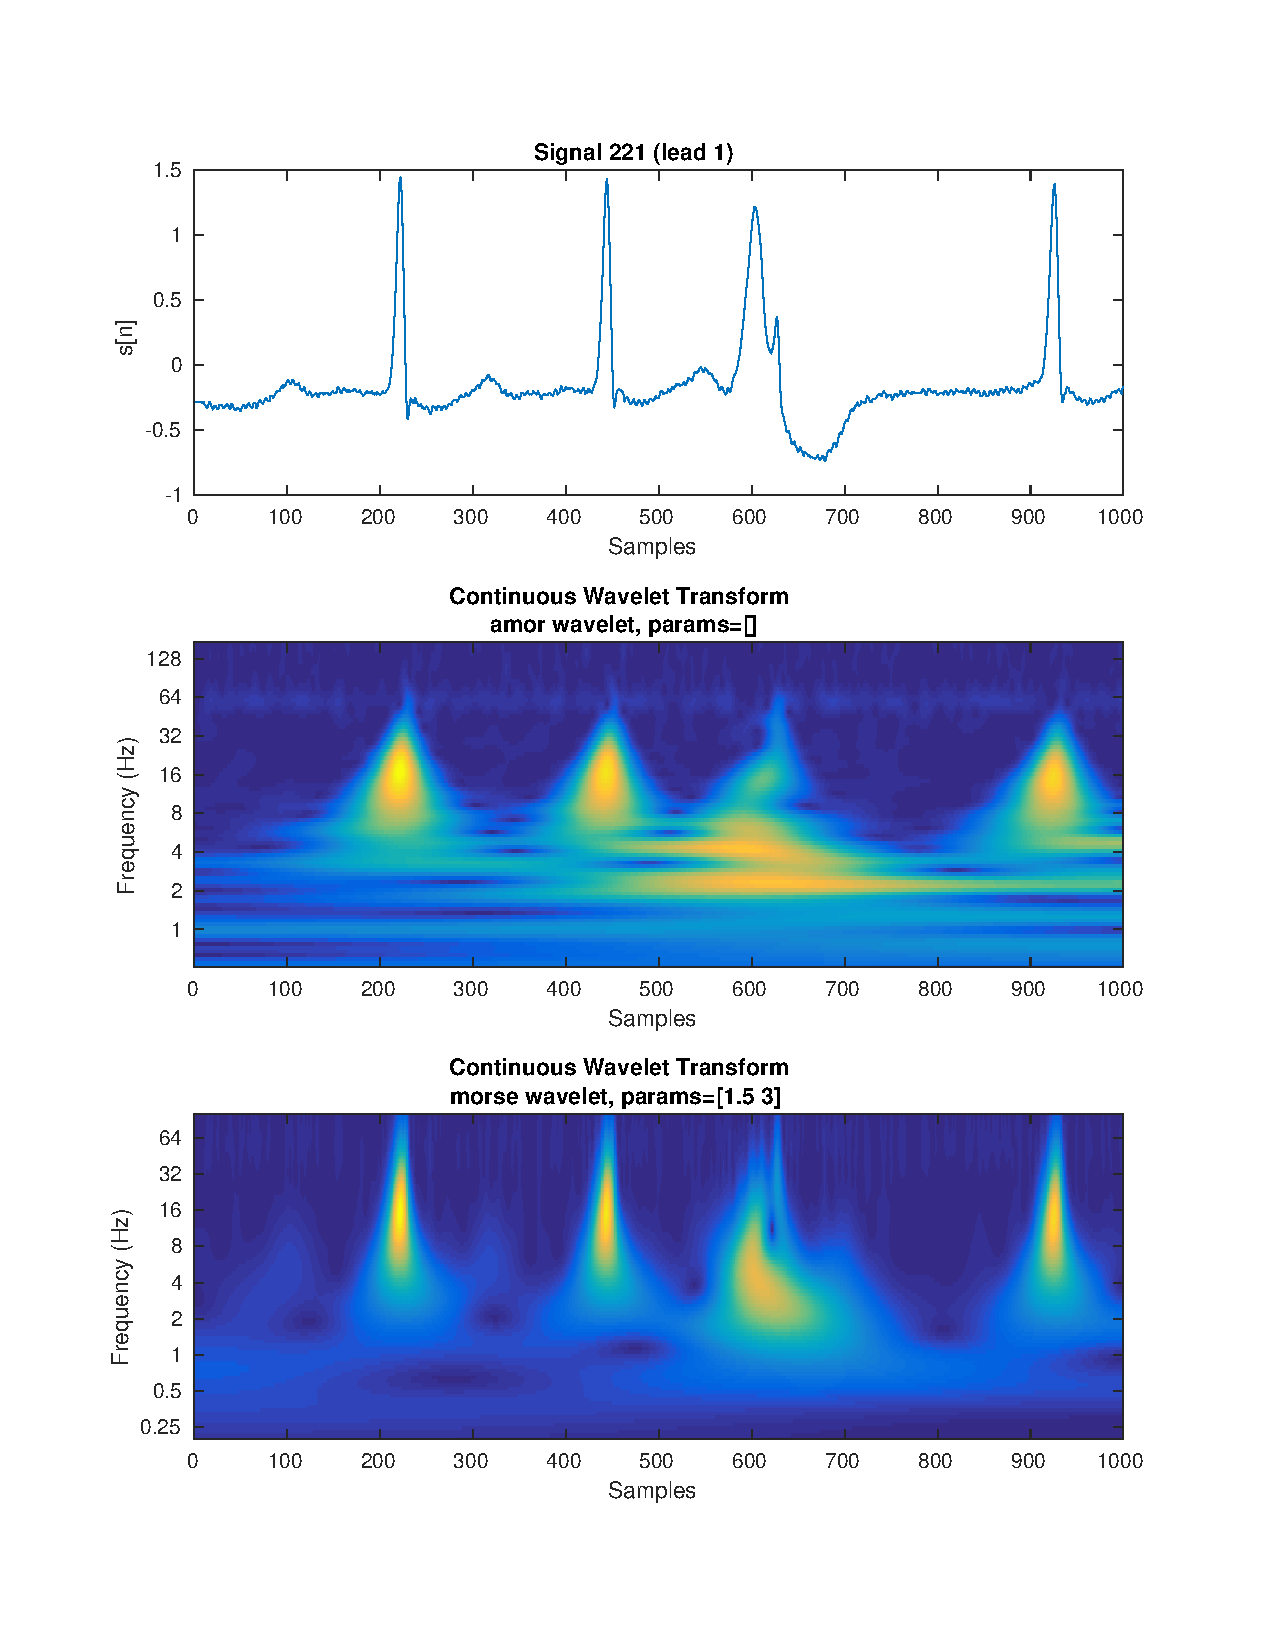
\includegraphics[width=\textwidth]{fig/221l1_cwt.pdf}
\end{figure}
\end{columns}
\end{frame}

\begin{frame}
\frametitle{Ανάλυση των σημάτων - 221}

\begin{columns}
\column{0.5\textwidth}
\begin{figure}
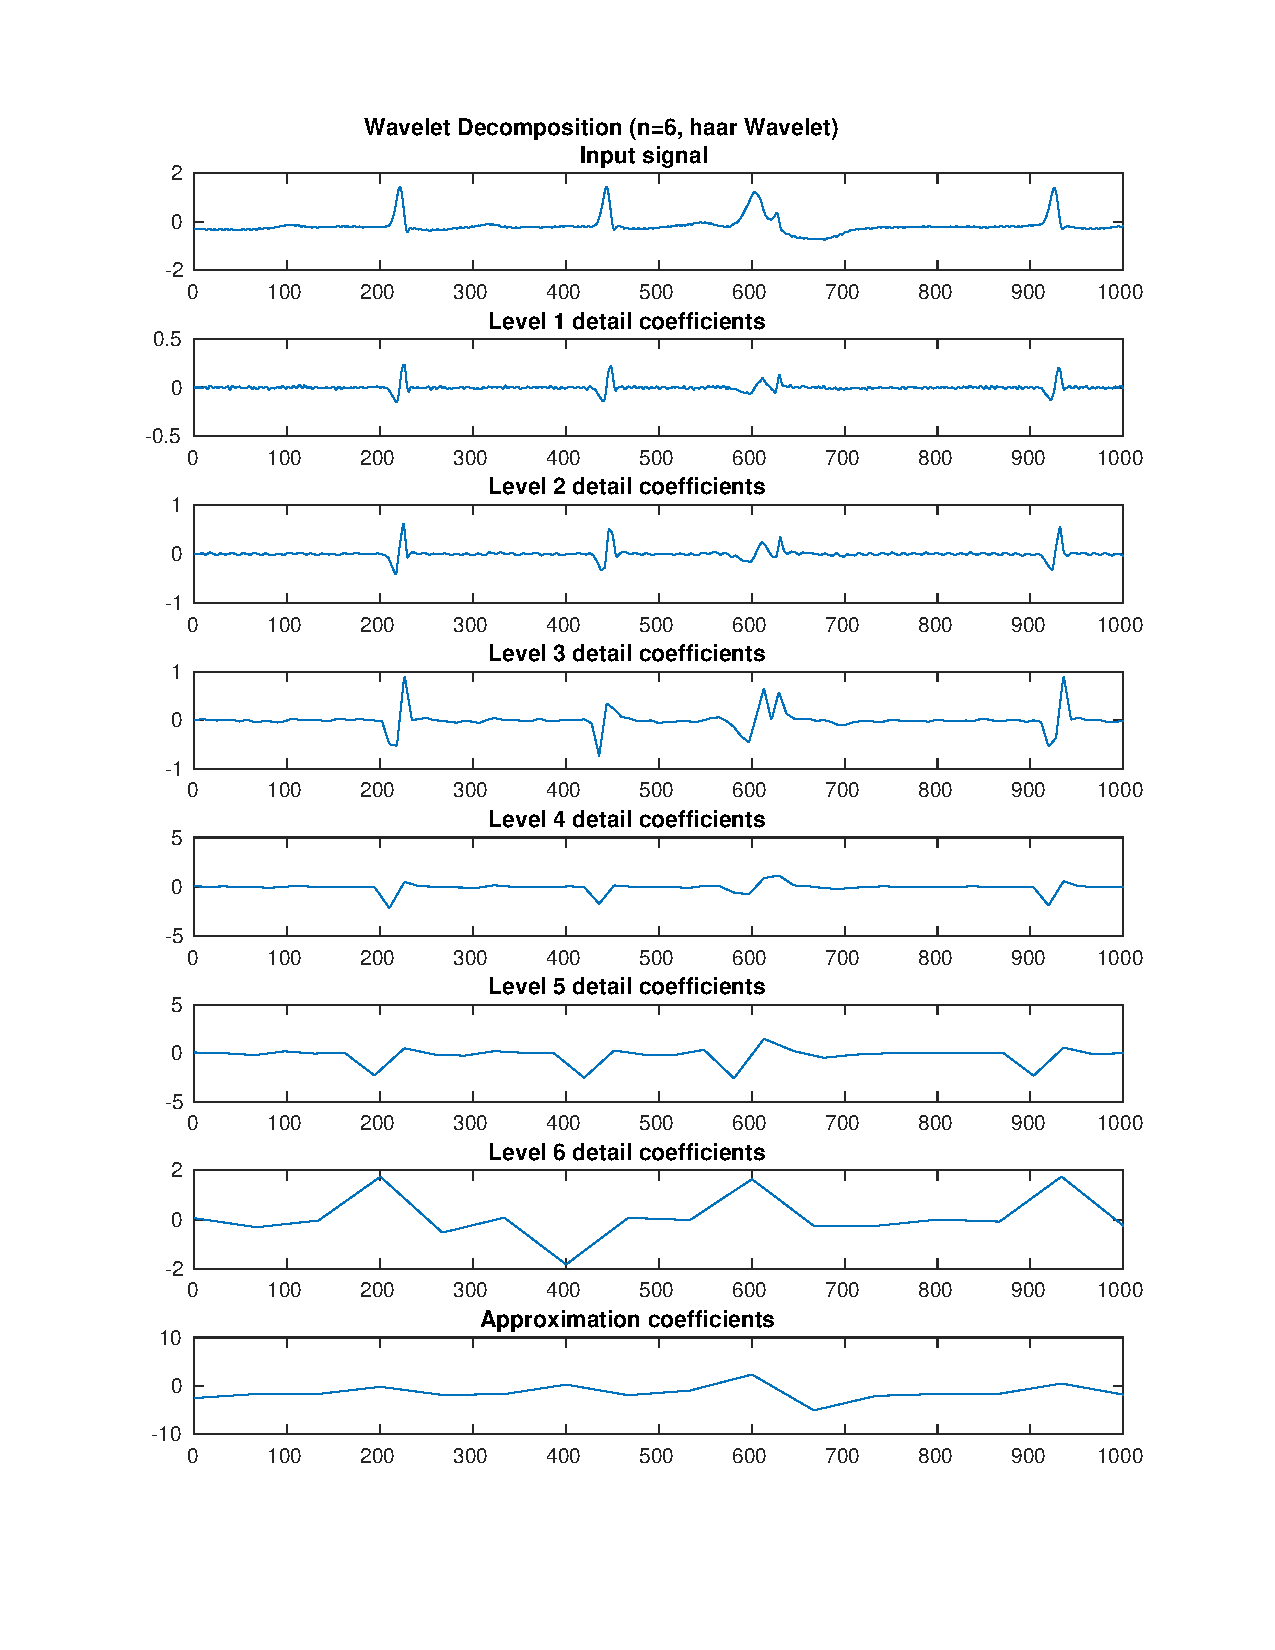
\includegraphics[width=\textwidth]{fig/221l1_dwt1.pdf}
\end{figure}

\column{0.5\textwidth}
\begin{figure}
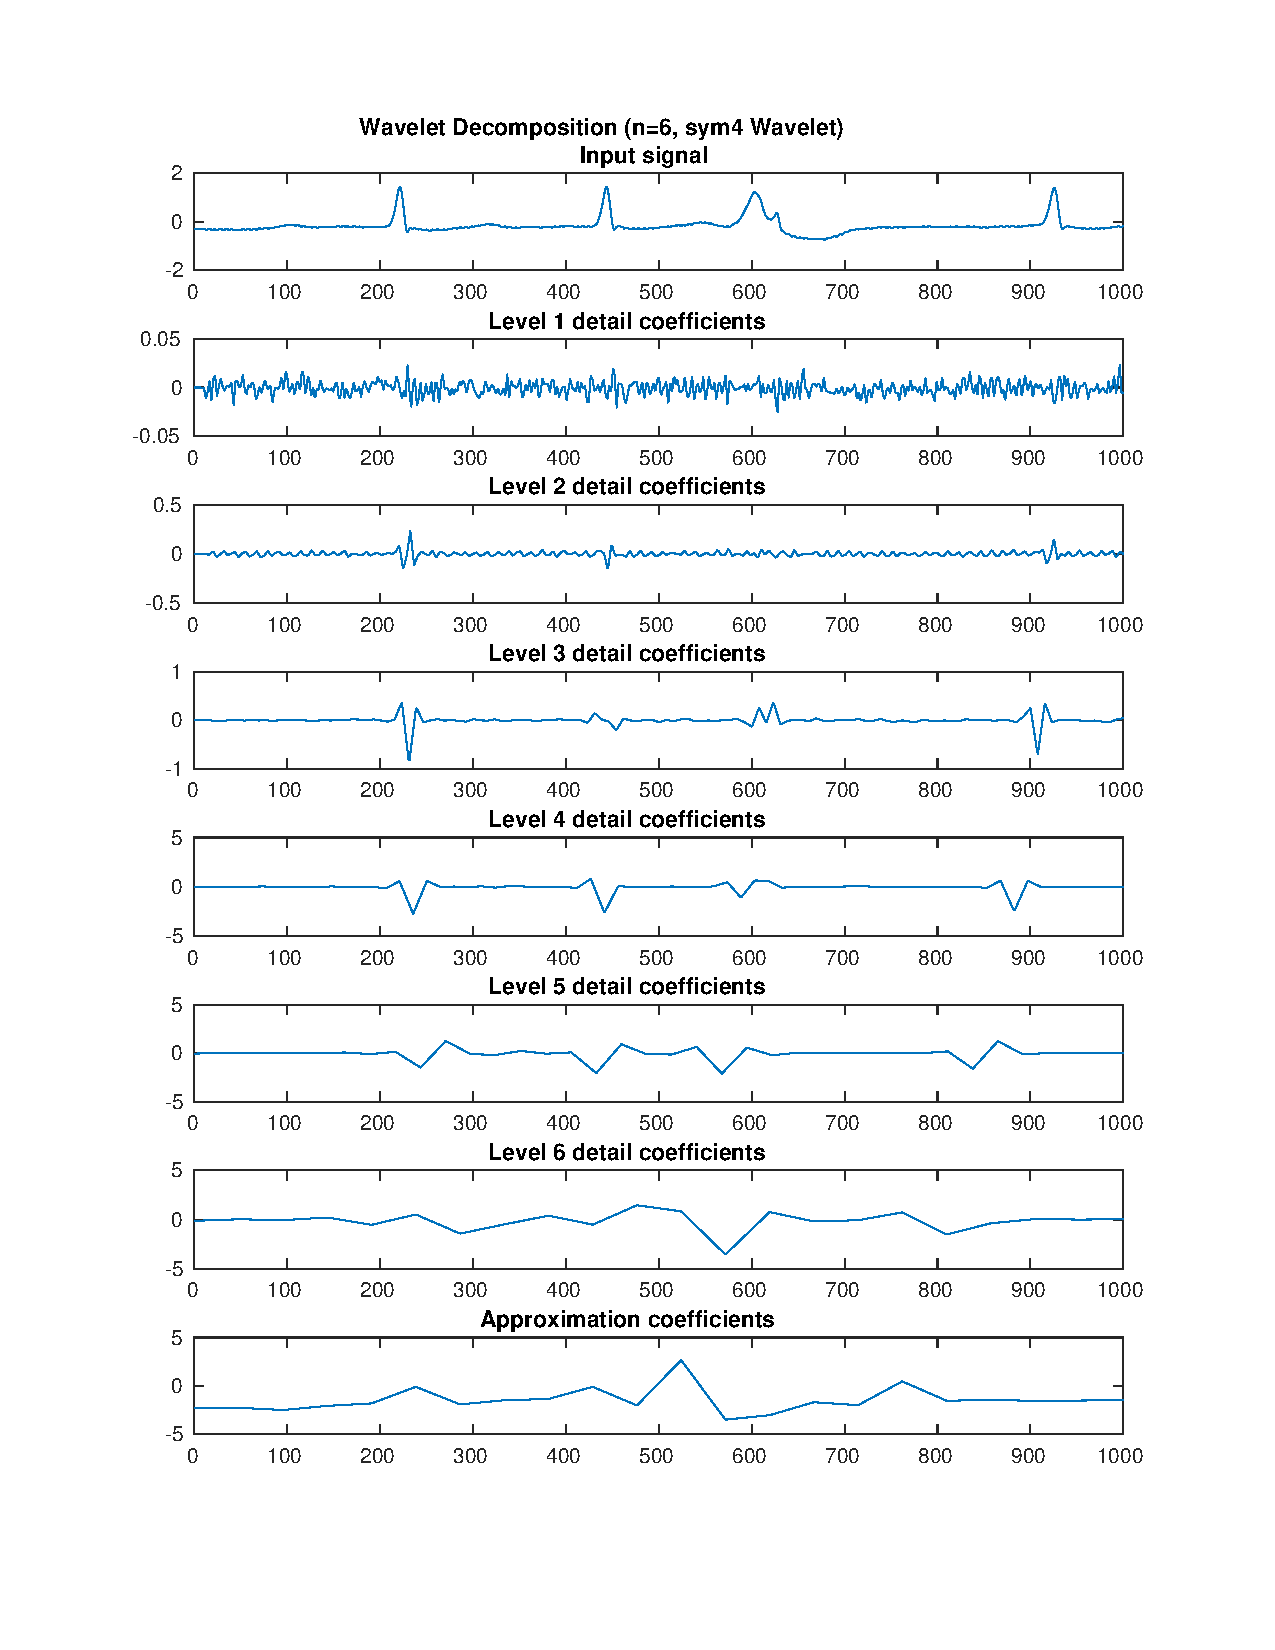
\includegraphics[width=\textwidth]{fig/221l1_dwt2.pdf}
\end{figure}
\end{columns}
\end{frame}

\begin{frame}
\frametitle{Ανάλυση των σημάτων - 221}

\begin{columns}
\column{0.5\textwidth}
\begin{figure}
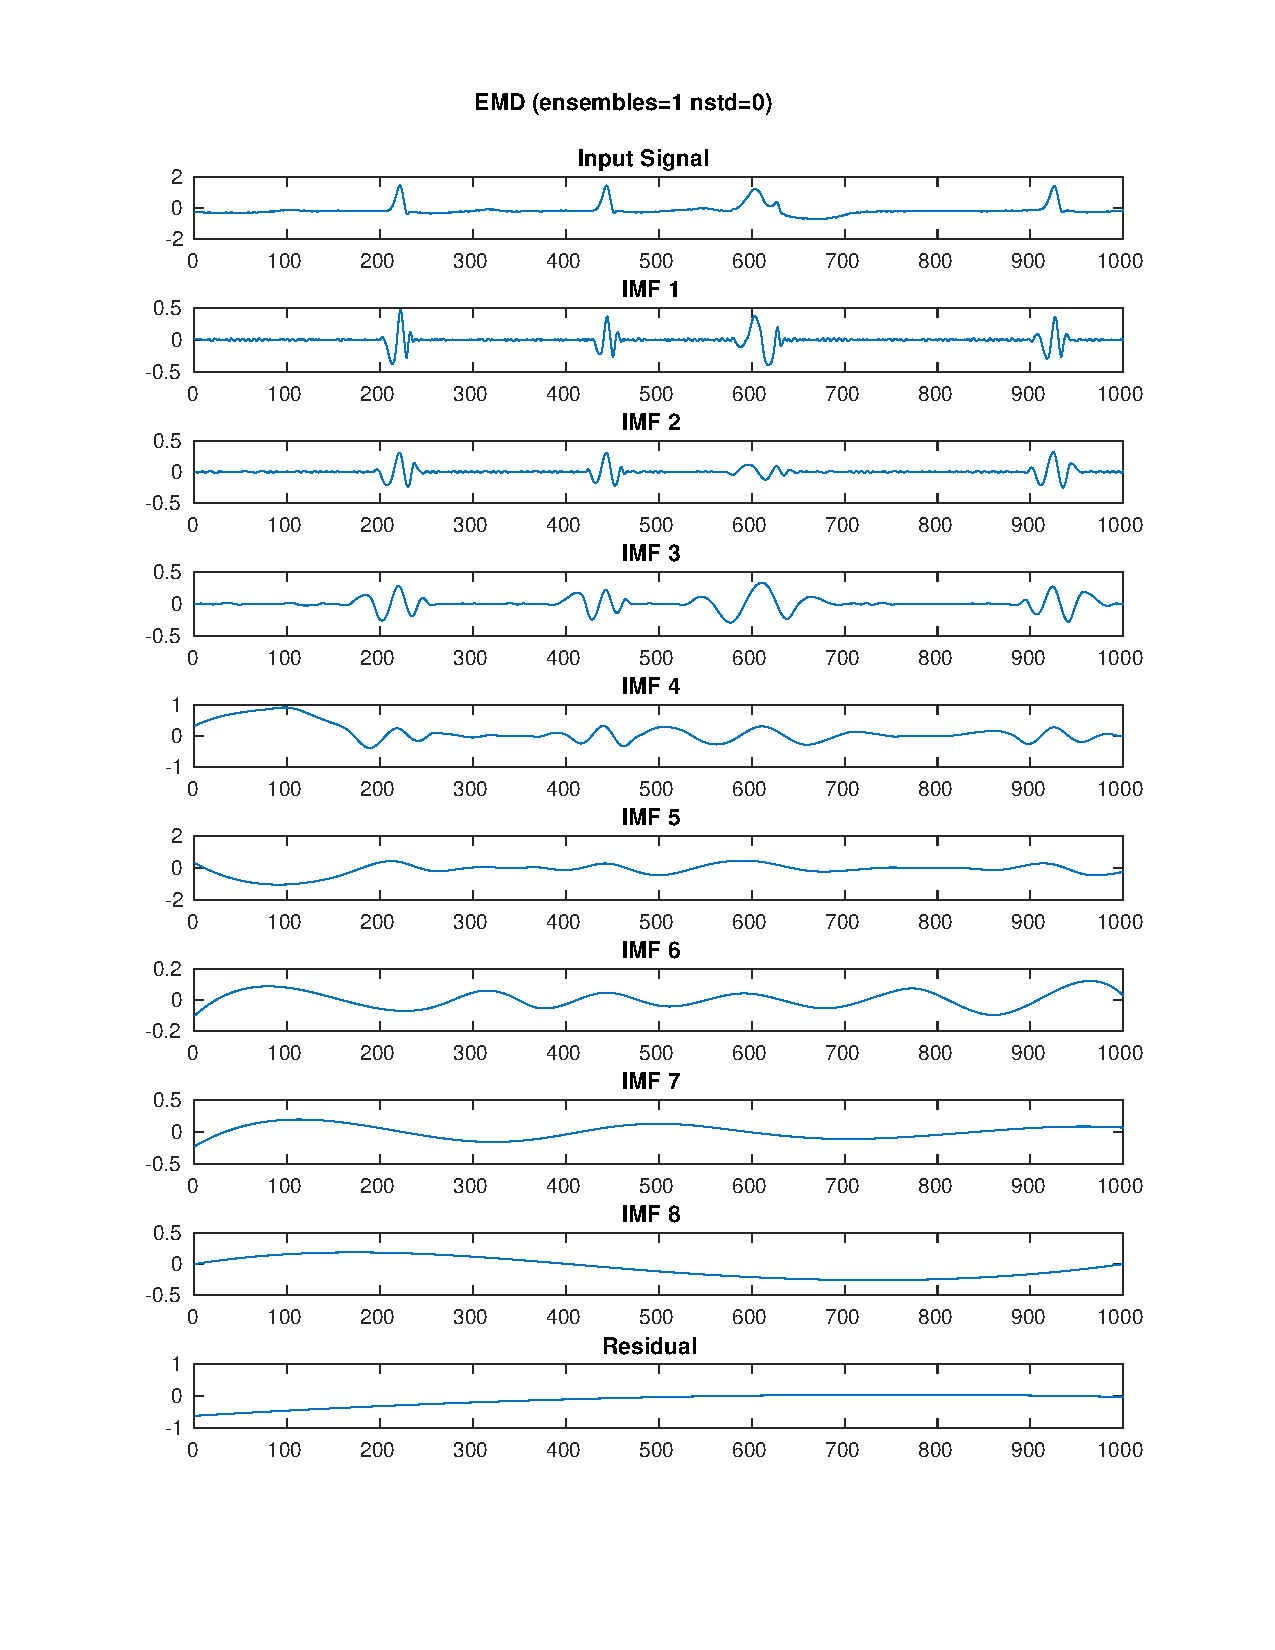
\includegraphics[width=\textwidth]{fig/221l1_emd.pdf}
\end{figure}

\column{0.5\textwidth}
\begin{figure}
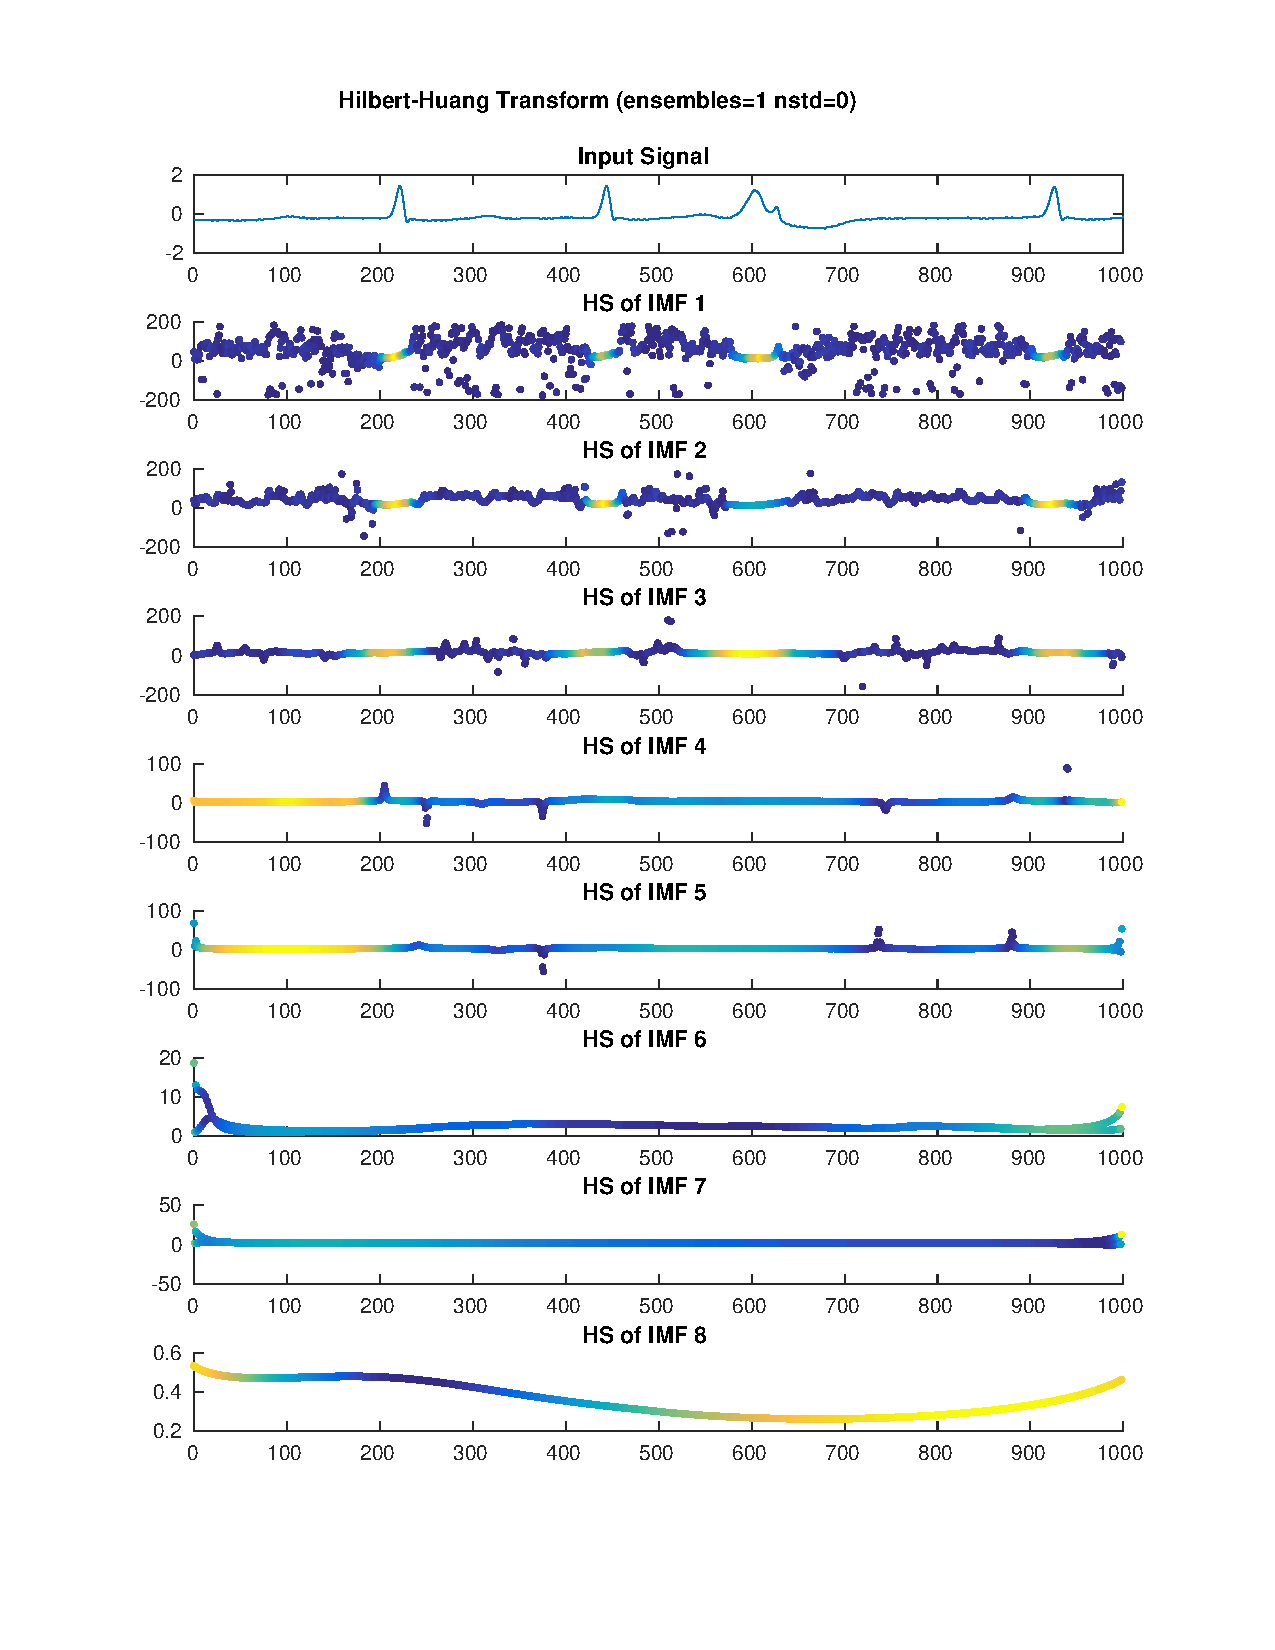
\includegraphics[width=\textwidth]{fig/221l1_hht.pdf}
\end{figure}
\end{columns}
\end{frame}


% --- Αλγόριθμος 1 ---
\section{Ανίχνευση Διαστημάτων R-R}
\subsection{Αλγόριθμος Ανίχνευσης}
\begin{frame}
\frametitle{Ανίχνευση διαστημάτων R-R}

\begin{itemize}
\item Κατασκευάσαμε δύο αλγορίθμους για ανίχνευση των διαστημάτων R-R.

	\setbeamertemplate{itemize items}[square]
	\begin{itemize}
	\item Ο πρώτος υπολογίζει το μέσο διάστημα R-R στο σήμα που του δίνεται.
	\item Ο δεύερος χρησιμοποιεί τον πρώτο για να ανιχνεύσει τις κορυφές R.
	\end{itemize}
	\setbeamertemplate{itemize items}[ball]
\end{itemize}

\begin{algorithm}[H]
  \scriptsize  
  \caption{Υπολογισμός μέσου εύρους διαστήματος R-R.}
  \label{alg:mean_rr_interval}  
  \begin{algorithmic}[1]  
    \Require{Δείγματα ECG $[s_1,s_2,...,s_N]$.}  
  	\Ensure{Μέσο εύρος $l_{R-R}$ του διαστήματος R-R.}
  	
  	\State Υπολόγισε τον συνεχή WT του σήματος s.
  	\State Μηδένισε τους συντελεστές που δεν ανήκουν στις κυρίαρχες συχνότητες 15-30Hz του QRS complex.
  	\State Άθροισε, για κάθε δείγμα, τα μέτρα των φιλτραρισμένων συντελεστών για να υπολογίσεις την ενέργεια του.
  	\State Υπολόγισε την αυτοσυσχέτιση της ενέργειας των δειγμάτων.
  	\State Βρες τη μέση διάρκεια του διαστήματος R-R από το δεύτερο τοπικό μέγιστο των συντελεστών της αυτοσυσχέτισης.
  	
  \end{algorithmic}  
\end{algorithm}
\end{frame}

%% -- Algorithm 1 images --
\begin{frame}
\frametitle{Ανίχνευση διαστημάτων R-R}

\centering
\begin{columns}
\column{0.4\textwidth}
\begin{figure}
\includegraphics[width=\textwidth, trim={0 6cm 0 6cm}, clip]{fig/filtered_wt.pdf}
\end{figure}

\column{0.4\textwidth}
\begin{figure}
\includegraphics[width=\textwidth, trim={0 6cm 0 6cm}, clip]{fig/wt_energy.pdf}
\end{figure}
\end{columns}

\begin{figure}
\includegraphics[width=0.4\textwidth, trim={0 6cm 0 6cm}, clip]{fig/autocorr_wt.pdf}
\end{figure}

\end{frame}


% --- Αλγόριθμος 2 ---
\begin{frame}
\frametitle{Ανίχνευση διαστημάτων R-R}

\begin{algorithm}[H]
  \scriptsize
  \caption{Ανίχνευση κορυφών R σε σήμα ECG.}
  \label{alg:detect_rr_intervals}  
  \begin{algorithmic}[1]  
    \Require{Δείγματα ECG $[s_1,s_2,...,s_N]$.}  
  	\Ensure{Διάνυσμα $[n_1,n_2,...,n_k]$ των δειγμάτων στα οποία εντοπίστηκαν κορυφές R.}
  	
  	\State Υπολόγισε τους συντελεστές του διακριτού WT, χρησιμοποιώντας το db6 κυματίδιο, για $n>5$ επίπεδα.
  	\State Ανακατασκεύασε το αρχικό σήμα χρησιμοποιώντας μόνο τους συντελεστές $d_{2-5}$, που περιέχουν το κύριο συχνοτικό περιεχόμενο των QRS complexes.
  	\State Υπολόγισε το τετράγωνο του ανακατασκευασμένου σήματος.
  	\State Υπολόγισε το μέσο διάστημα R-R, για ένα τμήμα του σήματος, με τον Αλγόριθμο \ref{alg:mean_rr_interval}.
  	\State Βρες τα τοπικά μέγιστα στο τετράγωνο του ανακατασκευασμένου σήματος, που απέχουν τουλάχιστον $80\%$ του μέσου διαστήματος $l_{R-R}$.
  	
  \end{algorithmic}  
\end{algorithm}
\end{frame}

%% -- Algorithm 2 images --
\begin{frame}
\frametitle{Ανίχνευση διαστημάτων R-R}

\begin{columns}

\centering
\column{0.5\textwidth}
\begin{figure}
\includegraphics[width=\textwidth, trim={0 3cm 0 2cm}, clip]{fig/detect_mra.pdf}
\end{figure}

\column{0.4\textwidth}
\begin{figure}
\includegraphics[width=0.8\textwidth, trim={2cm 7cm 2cm 7cm}, clip]{fig/reconstructed.pdf}
\end{figure}
\begin{figure}
\includegraphics[width=0.8\textwidth, trim={2cm 7cm 2cm 7cm}, clip]{fig/reconstructed_energy.pdf}
\end{figure}
\end{columns}

\end{frame}


%% -- Αποτελέσματα --
\subsection{Αποτελέσματα}
\begin{frame}
\frametitle{Ανίχνευση διαστημάτων R-R - Αξιολόγηση}

\begin{itemize}
\item Σε εύρος 20 δειγμάτων γύρω από τις πραγματικές κορυφές R, η κορυφή που ανιχνεύεται 	θεωρείται σωστή.
\item Με την υπόθεση αυτήν υπολογίζουμε τις TP, FN, FP εκτιμήσεις και την ακρίβεια του αλγορίθμου.
\end{itemize}

\centering
\begin{table}[H]

\resizebox{.8\textwidth}{!}{
\begin{tabular}{| c | c | c | c | c | c |}
 \hline
 Σήμα & TP & FN & FP & Accuracy & Χρόνος Εκτέλεσης \\ 
 \hline
 112 (Ακρ. 1) & 2536 & 1 & 2 & 99.88\% & 0.36s \\ 
 \hline
 112 (Ακρ. 2) & 2533 & 4 & 3 & 99.72\% & 0.36s \\ 
 \hline
 123 & 1482 & 33 & 0 & 97.82\% & 0.36s \\ 
 \hline
 118 & 2118 & 48 & 83 & 94.17\% & 0.35s \\ 
 \hline
 217 & 1992 & 54 & 104 & 92.65\% & 0.35s \\ 
 \hline
 221 & 2028 & 3 & 45 & 97.68\% & 0.35s \\ 
 \hline
\end{tabular}}
\end{table}

\end{frame}


%% -- Αποτελέσματα --
\begin{frame}
\frametitle{Ανίχνευση διαστημάτων R-R - Αποτελέσματα}

\centering
\begin{columns}
\column{0.5\textwidth}
\begin{figure}
\includegraphics[width=\textwidth, trim={1cm 6cm 1cm 6cm}, clip]{fig/112l1_detected_peaks.pdf}
\end{figure}

\column{0.5\textwidth}
\begin{figure}
\includegraphics[width=\textwidth, trim={1cm 6cm 1cm 6cm}, clip]{fig/112l2_detected_peaks.pdf}
\end{figure}
\end{columns}
\end{frame}

\begin{frame}
\frametitle{Ανίχνευση διαστημάτων R-R - Αποτελέσματα}

\begin{columns}
\centering
\column{0.5\textwidth}
\begin{figure}
\includegraphics[width=\textwidth, trim={1cm 6cm 1cm 6cm}, clip]{fig/123l1_detected_peaks.pdf}
\end{figure}

\column{0.5\textwidth}
\begin{figure}
\includegraphics[width=\textwidth, trim={1cm 6cm 1cm 6cm}, clip]{fig/118l1_detected_peaks.pdf}
\end{figure}
\end{columns}
\end{frame}

\begin{frame}
\frametitle{Ανίχνευση διαστημάτων R-R - Αποτελέσματα}

\begin{columns}
\centering
\column{0.5\textwidth}
\begin{figure}
\includegraphics[width=\textwidth, trim={1cm 6cm 1cm 6cm}, clip]{fig/217l1_detected_peaks.pdf}
\end{figure}

\column{0.5\textwidth}
\begin{figure}
\includegraphics[width=\textwidth, trim={1cm 6cm 1cm 6cm}, clip]{fig/221l1_detected_peaks.pdf}
\end{figure}
\end{columns}
\end{frame}


\end{document}